\section{Cylindrical Objects}
\label{sect:CylindricalObjects}

\subsection{Disc}
\label{sect:Disc}
\hspace{1pt} \\

\begin{figure}[htb]
\begin{center}
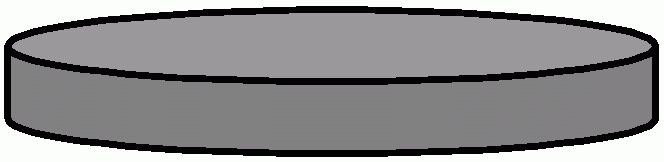
\includegraphics[width=0.5\textwidth,height=0.07188\textwidth]{../images/form_factor/cylindrical_obj/disc.png}
\end{center}
\caption{} \label{disc}
\end{figure}
\begin{align}
I_\text{Disc}(q,R)=\pi^2R^4\Delta\eta^2\frac{2}{(qR)^2}
\left(1-\frac{1}{qR}\text{J}_1(2qR)\right)
\end{align}
with $\DS \lim_{q=0}I_\text{Disc}(q,R) = \pi^2R^4\Delta\eta^2$

\vspace{5mm}

\underline{Input Parameters for model \texttt{Disc}:}
\begin{description}
\item[\texttt{R}] radius of disc $R$
\item[\texttt{eta}] scattering contrast $\Delta\eta$
\end{description}

\noindent\underline{Note:}
\begin{itemize}
\item none
\end{itemize}

\begin{figure}[htb]
\begin{center}
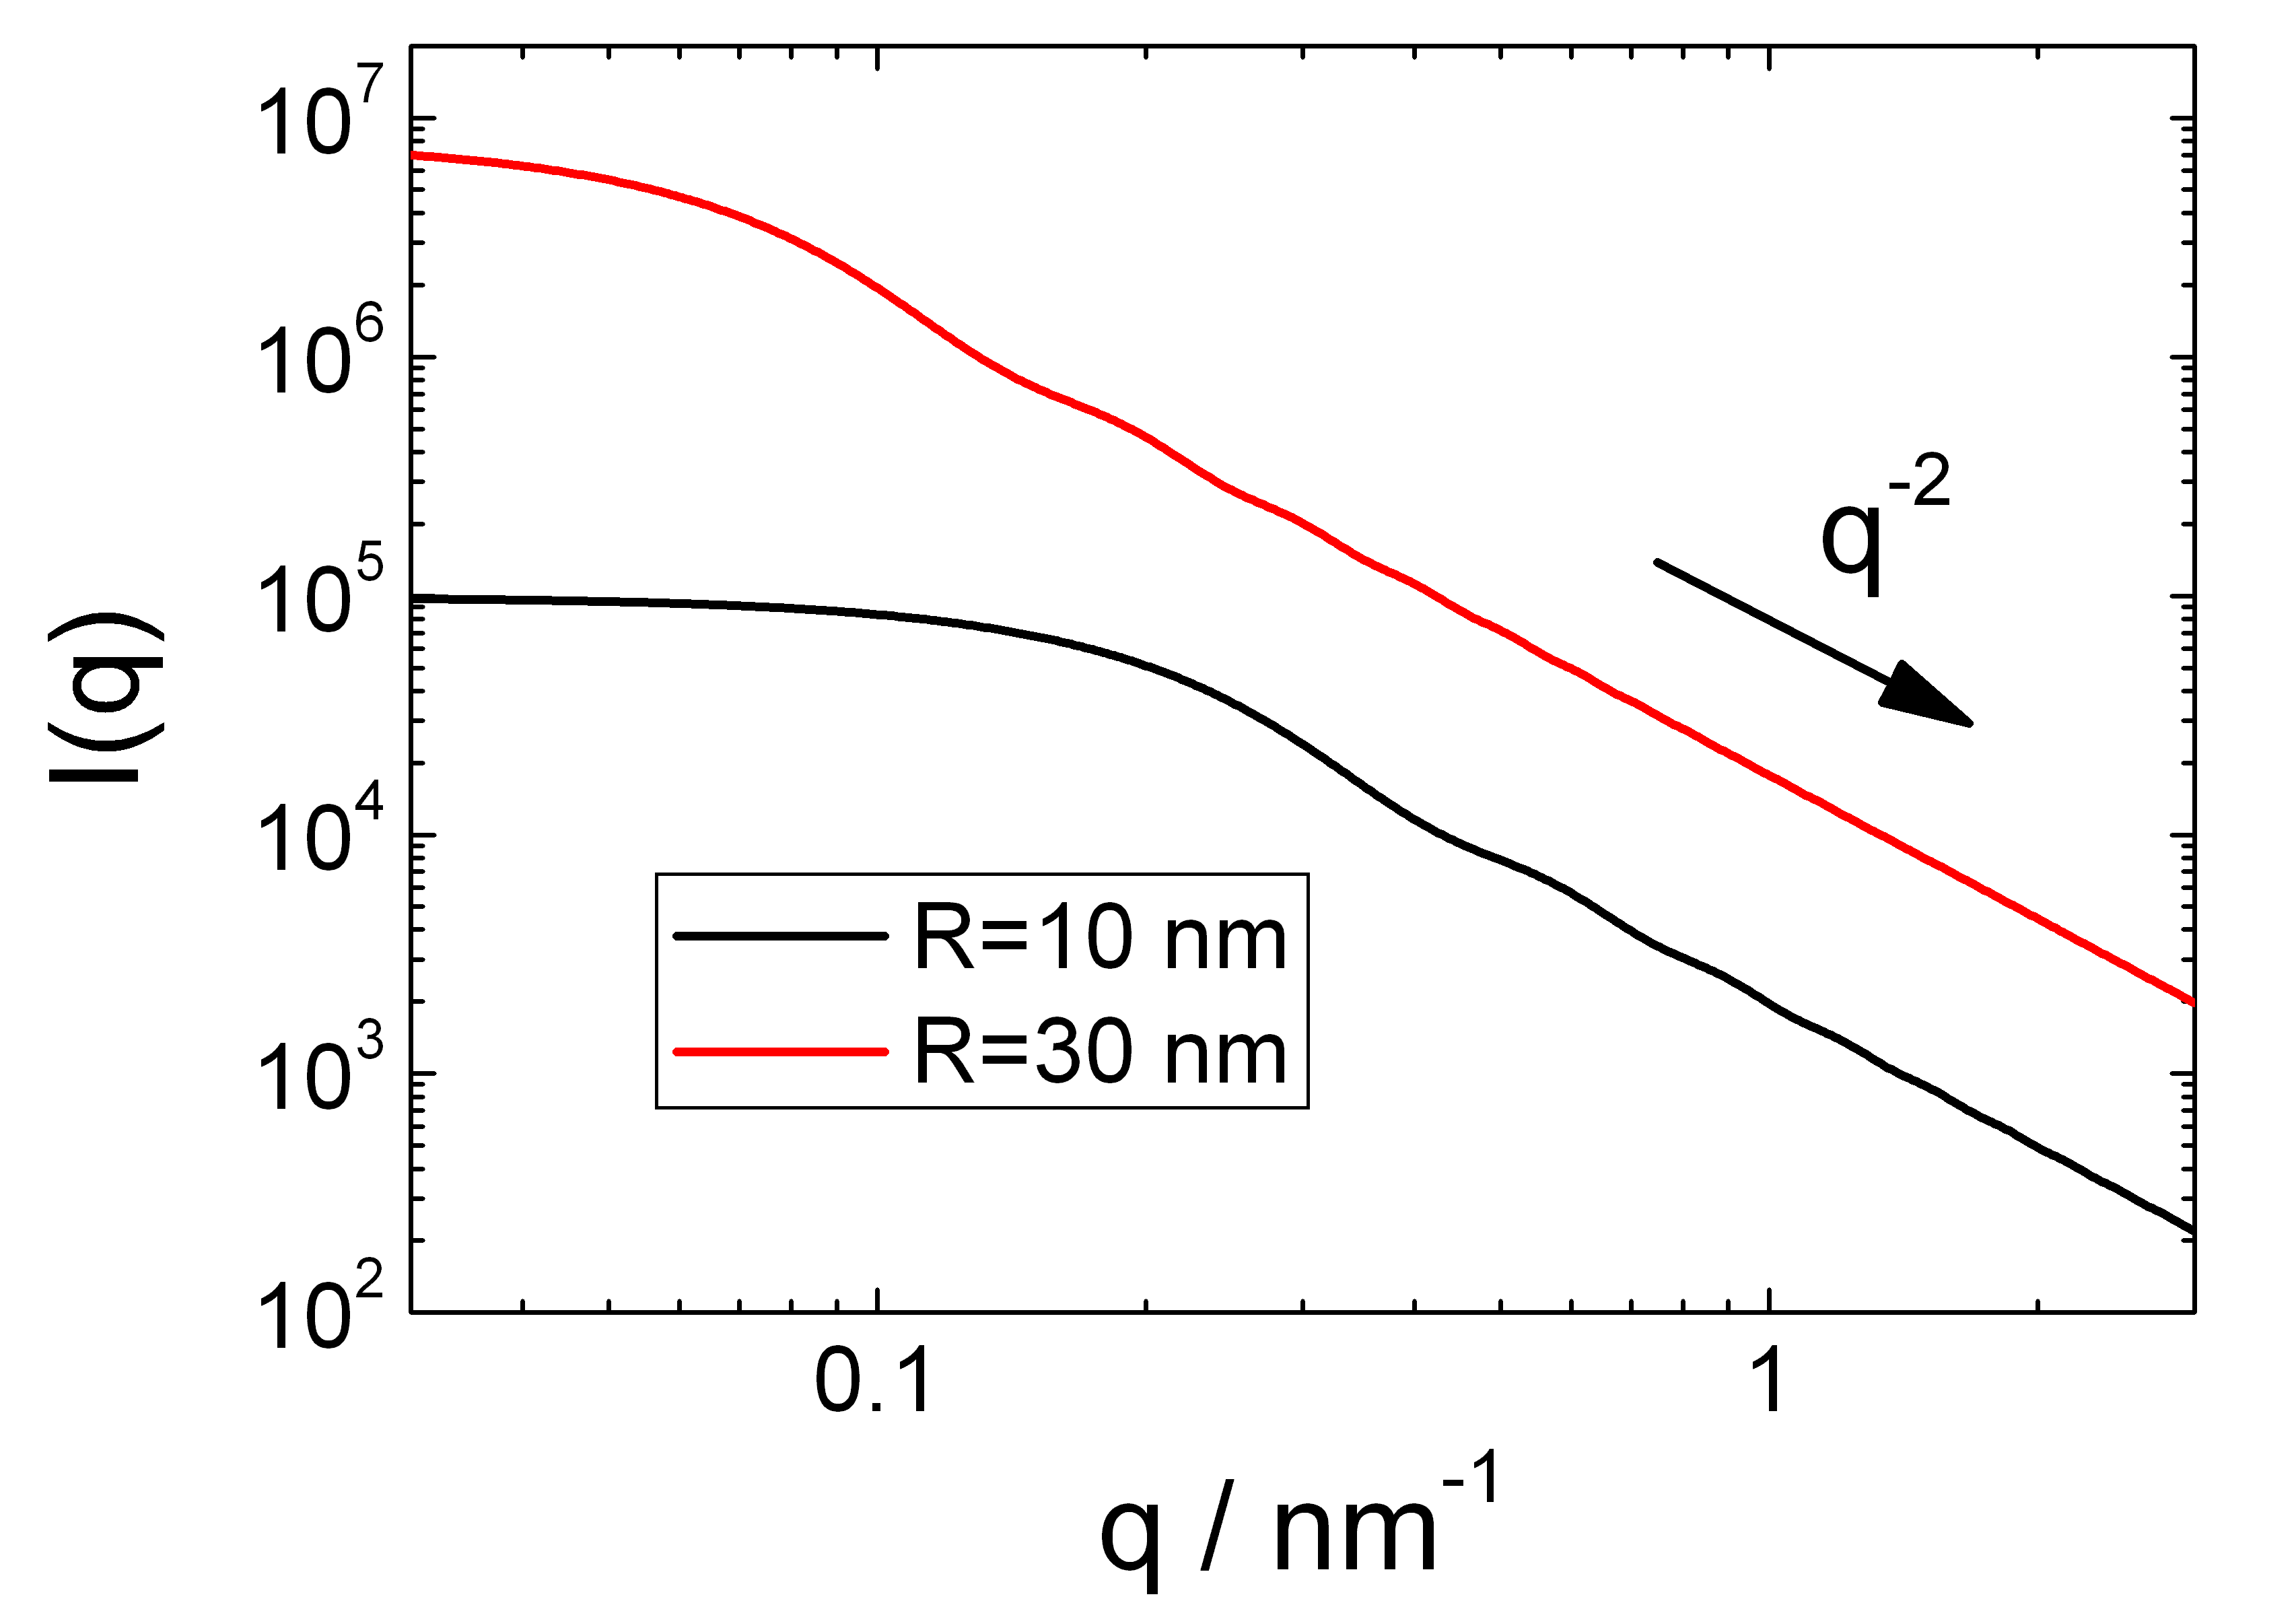
\includegraphics[width=0.668\textwidth,height=0.488\textwidth]{../images/form_factor/cylindrical_obj/DiscIQ.png}
\end{center}
\caption{Scattering intensity of a disc with radii $R=10$ nm and $R=30$ nm.
The scattering length density contrast is set to 1.}
\label{fig:I_disc}
\end{figure}

%%%%%%%%%%%%%%%%%%%%%%%%%%%%%%%%%%%%%%%%%%%%%%%%%%%%%%%%%%%%%%%%%

\newpage
\subsection{Rod}
\label{sect:Rod}
~\\

\begin{figure}[htb]
\begin{center}
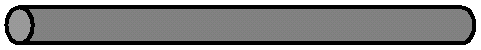
\includegraphics[width=0.5\textwidth,height=0.05194\textwidth]{../images/form_factor/cylindrical_obj/rod.png}
\end{center}
\caption{} \label{rod}
\end{figure}
\begin{align}
I_\text{Rod}(q,L) = \Delta\eta^2L^2\left(\frac{2}{qL}\text{Si}(qL)
                                         - \frac{\sin(qL/2)}{qL/2}
                                   \right)
\end{align}
with $\DS \text{Si}(x)=\int_0^x\!\frac{\sin t}{t}\,\,dt$ and $\DS
\lim_{q=0} I_\text{Rod}(q,L) = \Delta\eta^2L^2$

\vspace{5mm}

\underline{Input Parameters for model \texttt{Rod}:}
\begin{description}
\item[\texttt{L}] length of rod $L$
\item[\texttt{eta}] scattering contrast $\Delta\eta$
\end{description}

\underline{Note:}
\begin{itemize}
\item none
\end{itemize}

\begin{figure}[htb]
\begin{center}
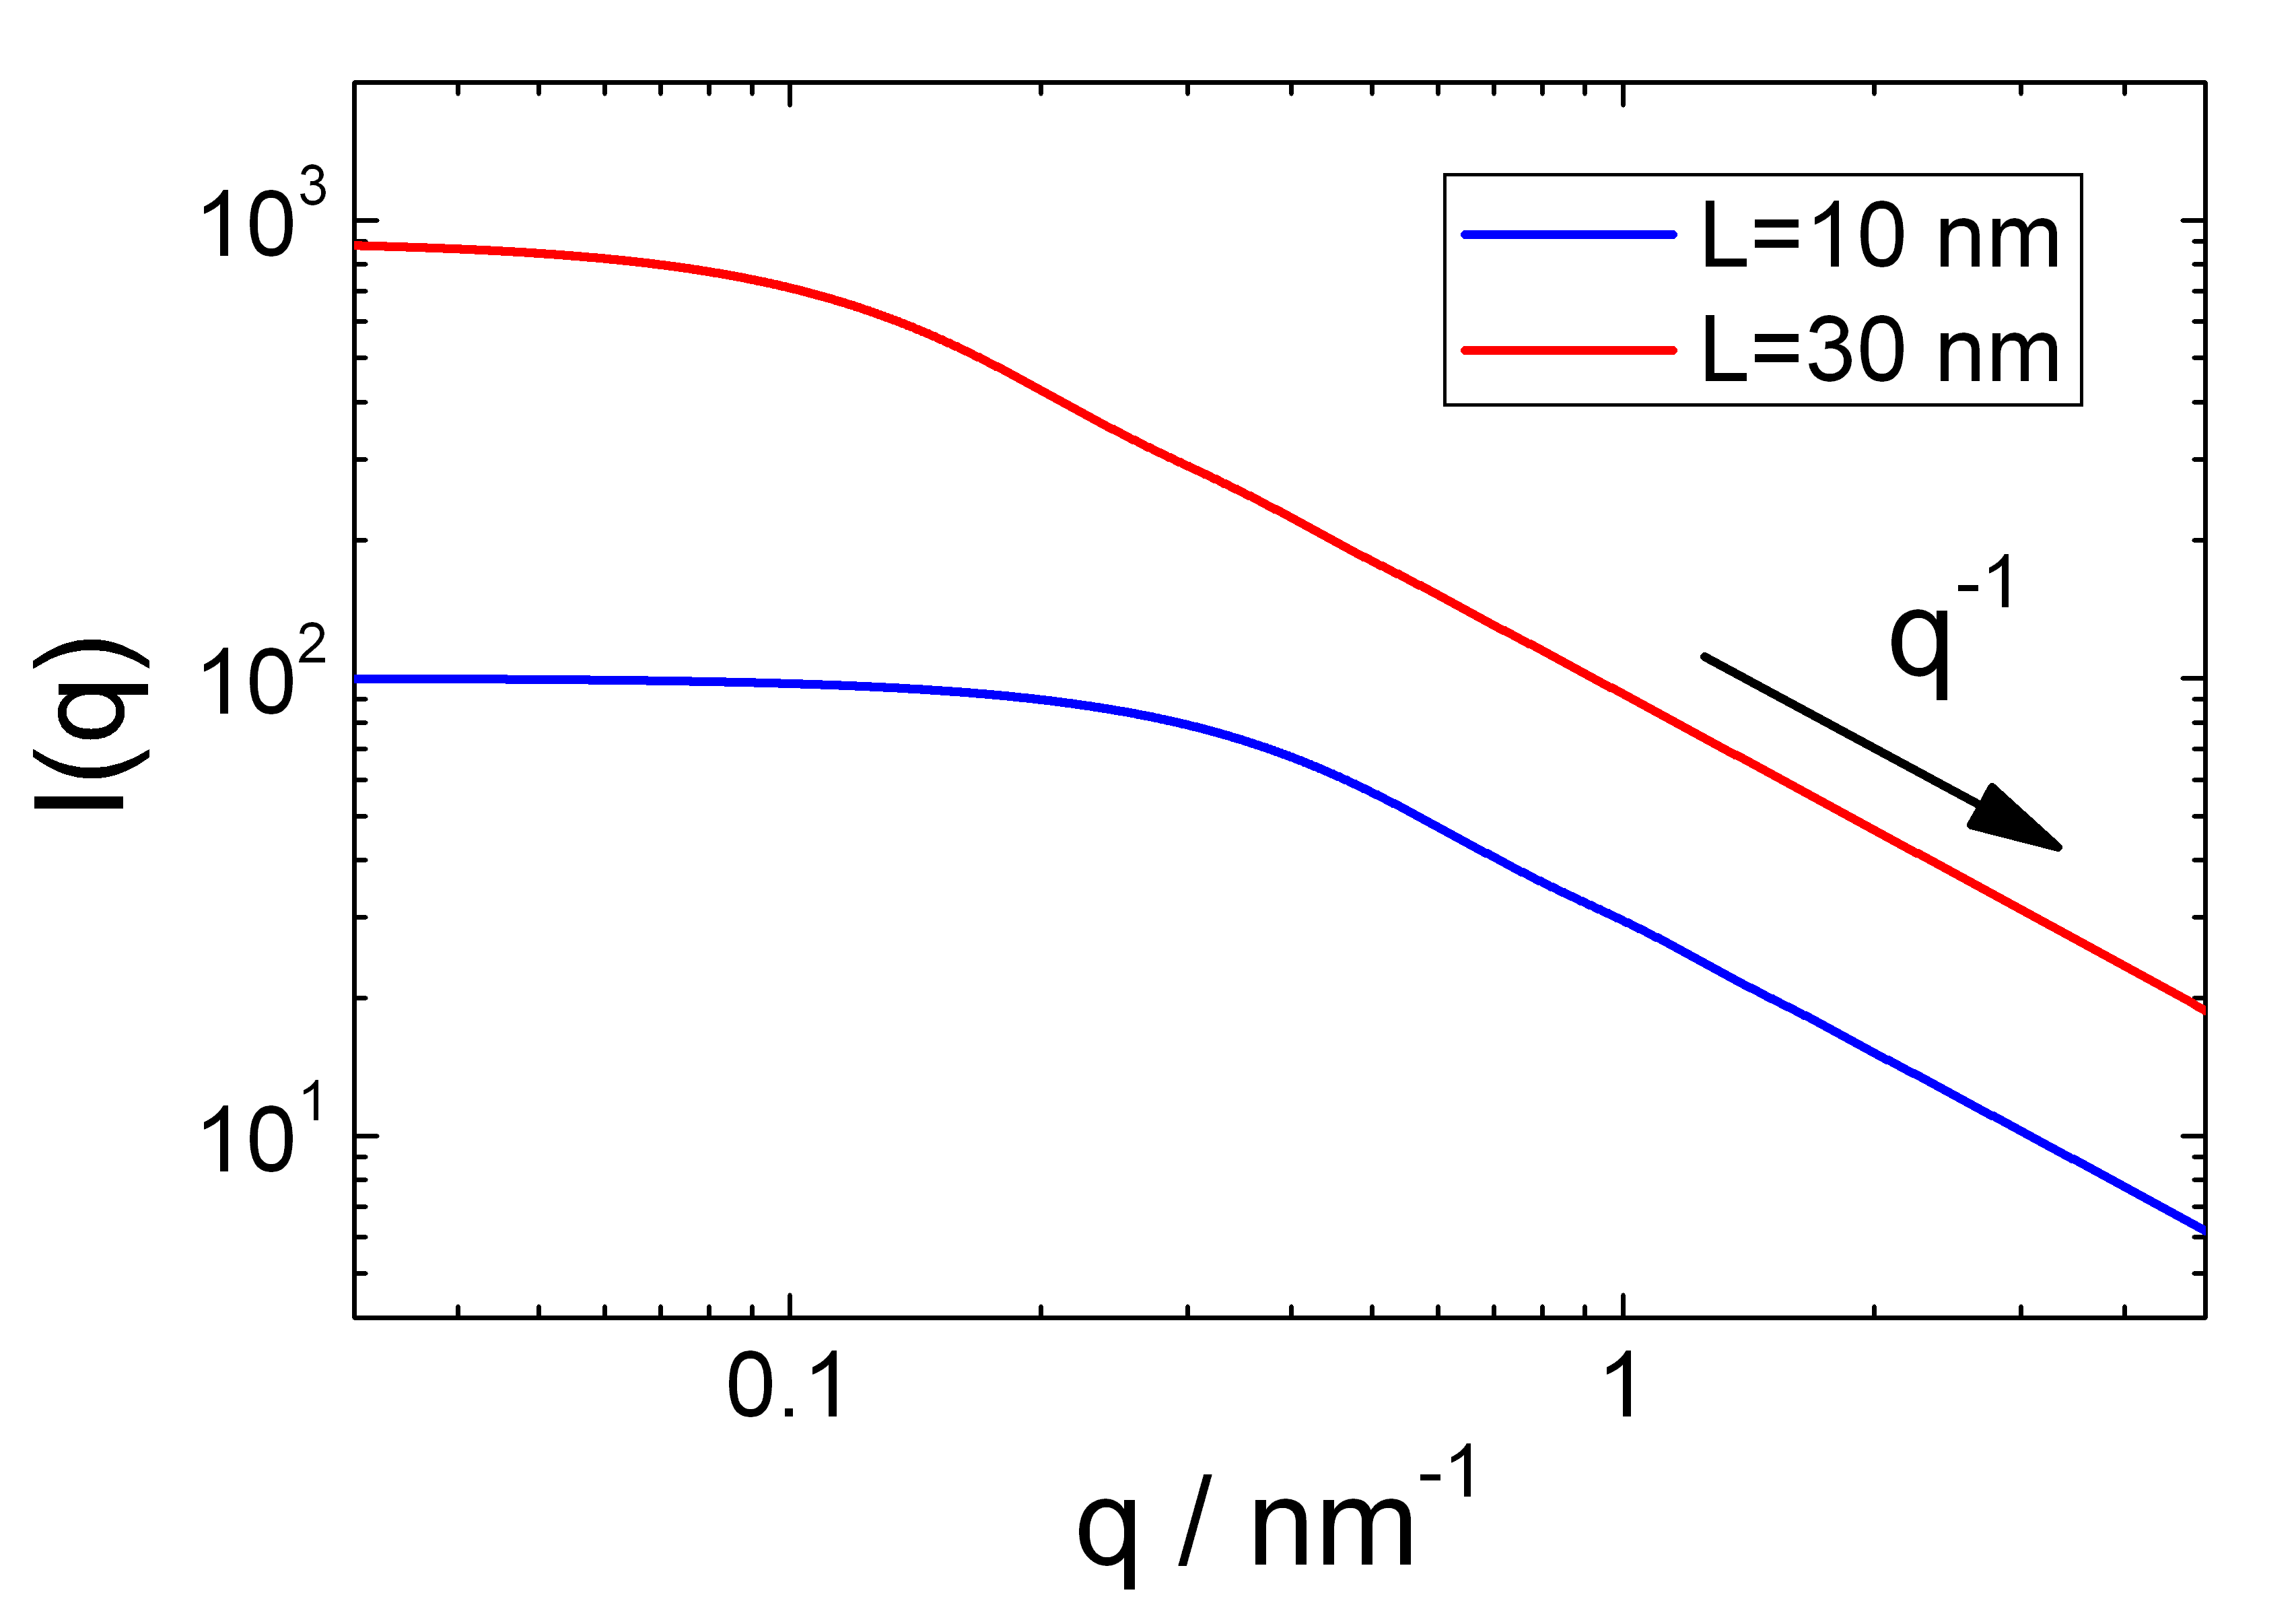
\includegraphics[width=0.668\textwidth,height=0.488\textwidth]{../images/form_factor/cylindrical_obj/RodIQ.png}
\end{center}
\caption{Scattering intensity of a rod of length $L=10$ nm and $L=30$ nm.
The scattering length density contrast is set to 1.}
\label{fig:I_rod}
\end{figure}
%%%%%%%%%%%%%%%%%%%%%%%%%%%%%%%%%%%%%%%%%%%%%%%%%%%%%%%%%%%%%%%%%%%%%%

\clearpage
\subsection{Porod's approximation for a long cylinder \cite{Porod1948}}
\label{sect:LongCylinder}
~\\

\begin{figure}[htb]
\begin{center}
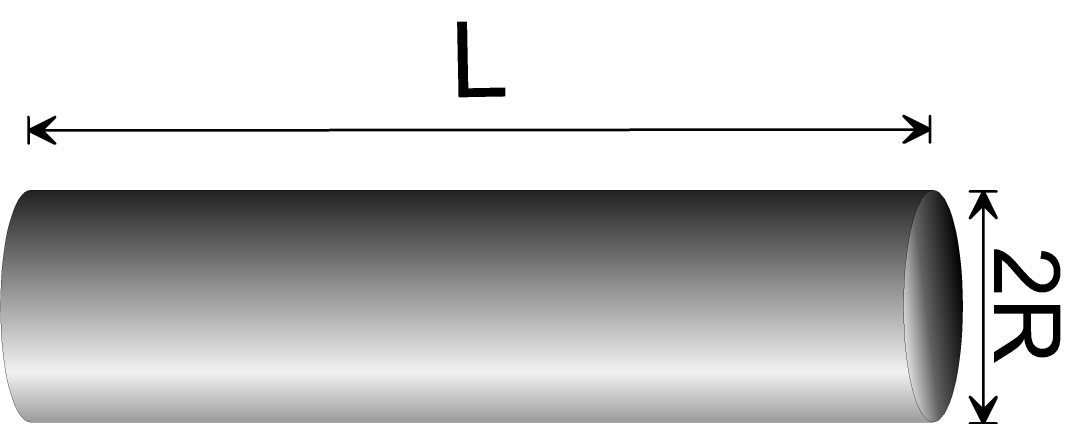
\includegraphics[width=0.8\textwidth,height=0.315\textwidth]{../images/form_factor/cylindrical_obj/long_cylinder.png}
\end{center}
\caption{} \label{longcylinder}
\end{figure}

\begin{align}
\text{Si}_\frac{\pi}{2}(x) &= \left( \mathrm{Si}(x)+\frac{\cos x}{x}+\frac{\sin x}{x^2} \right)
\quad \xrightarrow{x \rightarrow\infty} \quad \frac{\pi}{2} \\
\Lambda_1(x) &= \frac{2}{x} \mathrm{J}_1(x) \\
\Lambda_2(x) &= \frac{8}{x^2} \mathrm{J}_2(x) \\
\omega(x) &= \frac{8}{x^2} \left(3 \mathrm{J}_2(x) +\mathrm{J}_0(x)-1\right) \\
%\Phi_\text{disc}(x) &= \frac{2}{x^2}
%\left[1-\Lambda_1(x)\right] \\
\Phi_\text{long}(q,R,L) &= \left(\Delta\eta\pi
R^2L\right)^2 \frac{2}{QL}  \label{eq:LongCylinder}\\
& \quad \times \left\{\text{Si}_\frac{\pi}{2}(QL)\Lambda_1^2(QR)
%-\frac{2\Lambda_2(2QR)-\Phi_\text{disc}(2QR)}{QL}
-\frac{\omega(2QR)}{QL}
-\frac{\sin(QL)}{(QL)^2}\right\}\nonumber
\end{align}
$\mathrm{J}_n(x)$ are the regular cylindrical Bessel function of order $n$.

\vspace{5mm}

\underline{Input Parameters for model \texttt{LongCylinder}:}
\begin{description}
\item[\texttt{R}] radius of cylinder $R$
\item[\texttt{L}] length of cylinder $L$
\item[\texttt{eta}] scattering contrast $\Delta\eta$
\end{description}

\underline{Note:}
\begin{itemize}
\item The approximation is valid for $L>2R$
\end{itemize}

\begin{figure}[htb]
\begin{center}
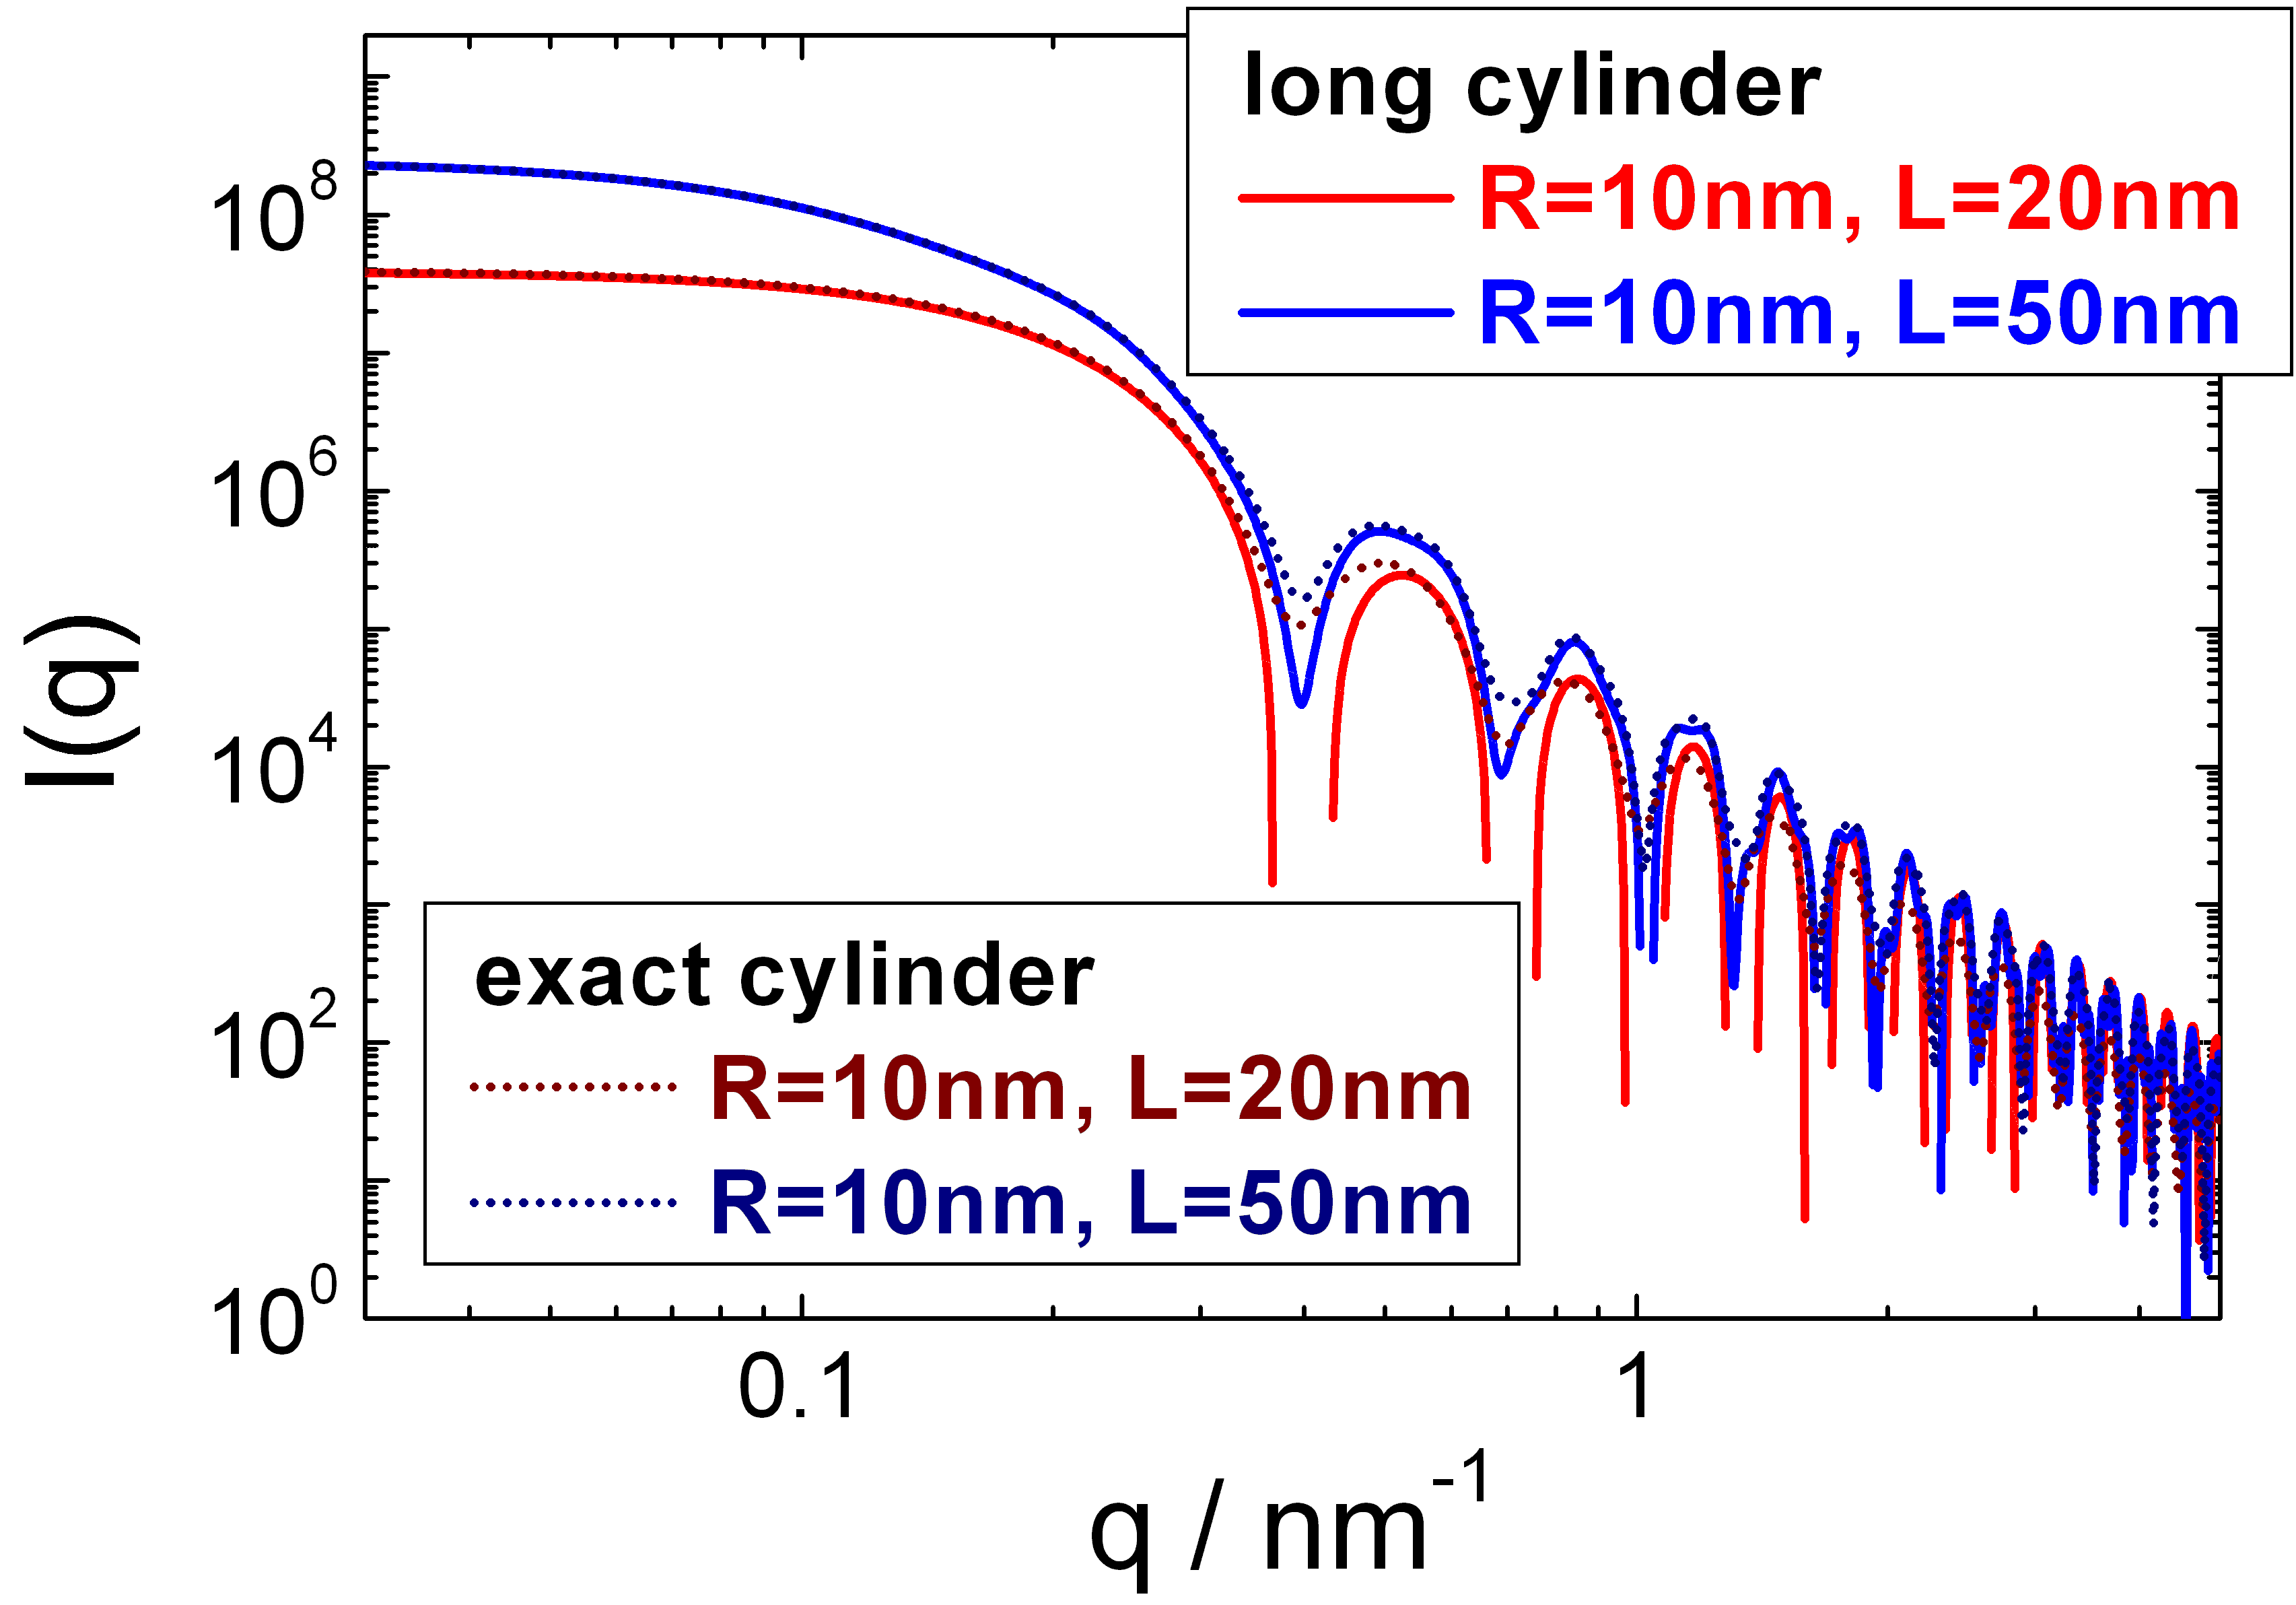
\includegraphics[width=0.668\textwidth,height=0.488\textwidth]{../images/form_factor/cylindrical_obj/LongCylinder.png}
\end{center}
\caption{Scattering intensity of a cylinder with radius $R=10$ nm and lengths of $L=20$ nm
and $L=50$ nm. Next to Porod's axproximation for long cylinders also
the exact integral solution is shown for comparison.
The scattering length density contrast is set to 1.}
\label{fig:LongCylinder}
\end{figure}

%%%%%%%%%%%%%%%%%%%%%%%%%%%%%%%%%%%%%%%%%%%%%%%%%%%%%%%%%%%%%%%%%%%%%%%%%%%%%%%%

\clearpage
\subsection{Porod's approximation for a flat cylinder \cite{Porod1948}}
\label{sect:flatCylinder}
~\\

\begin{figure}[htb]
\begin{center}
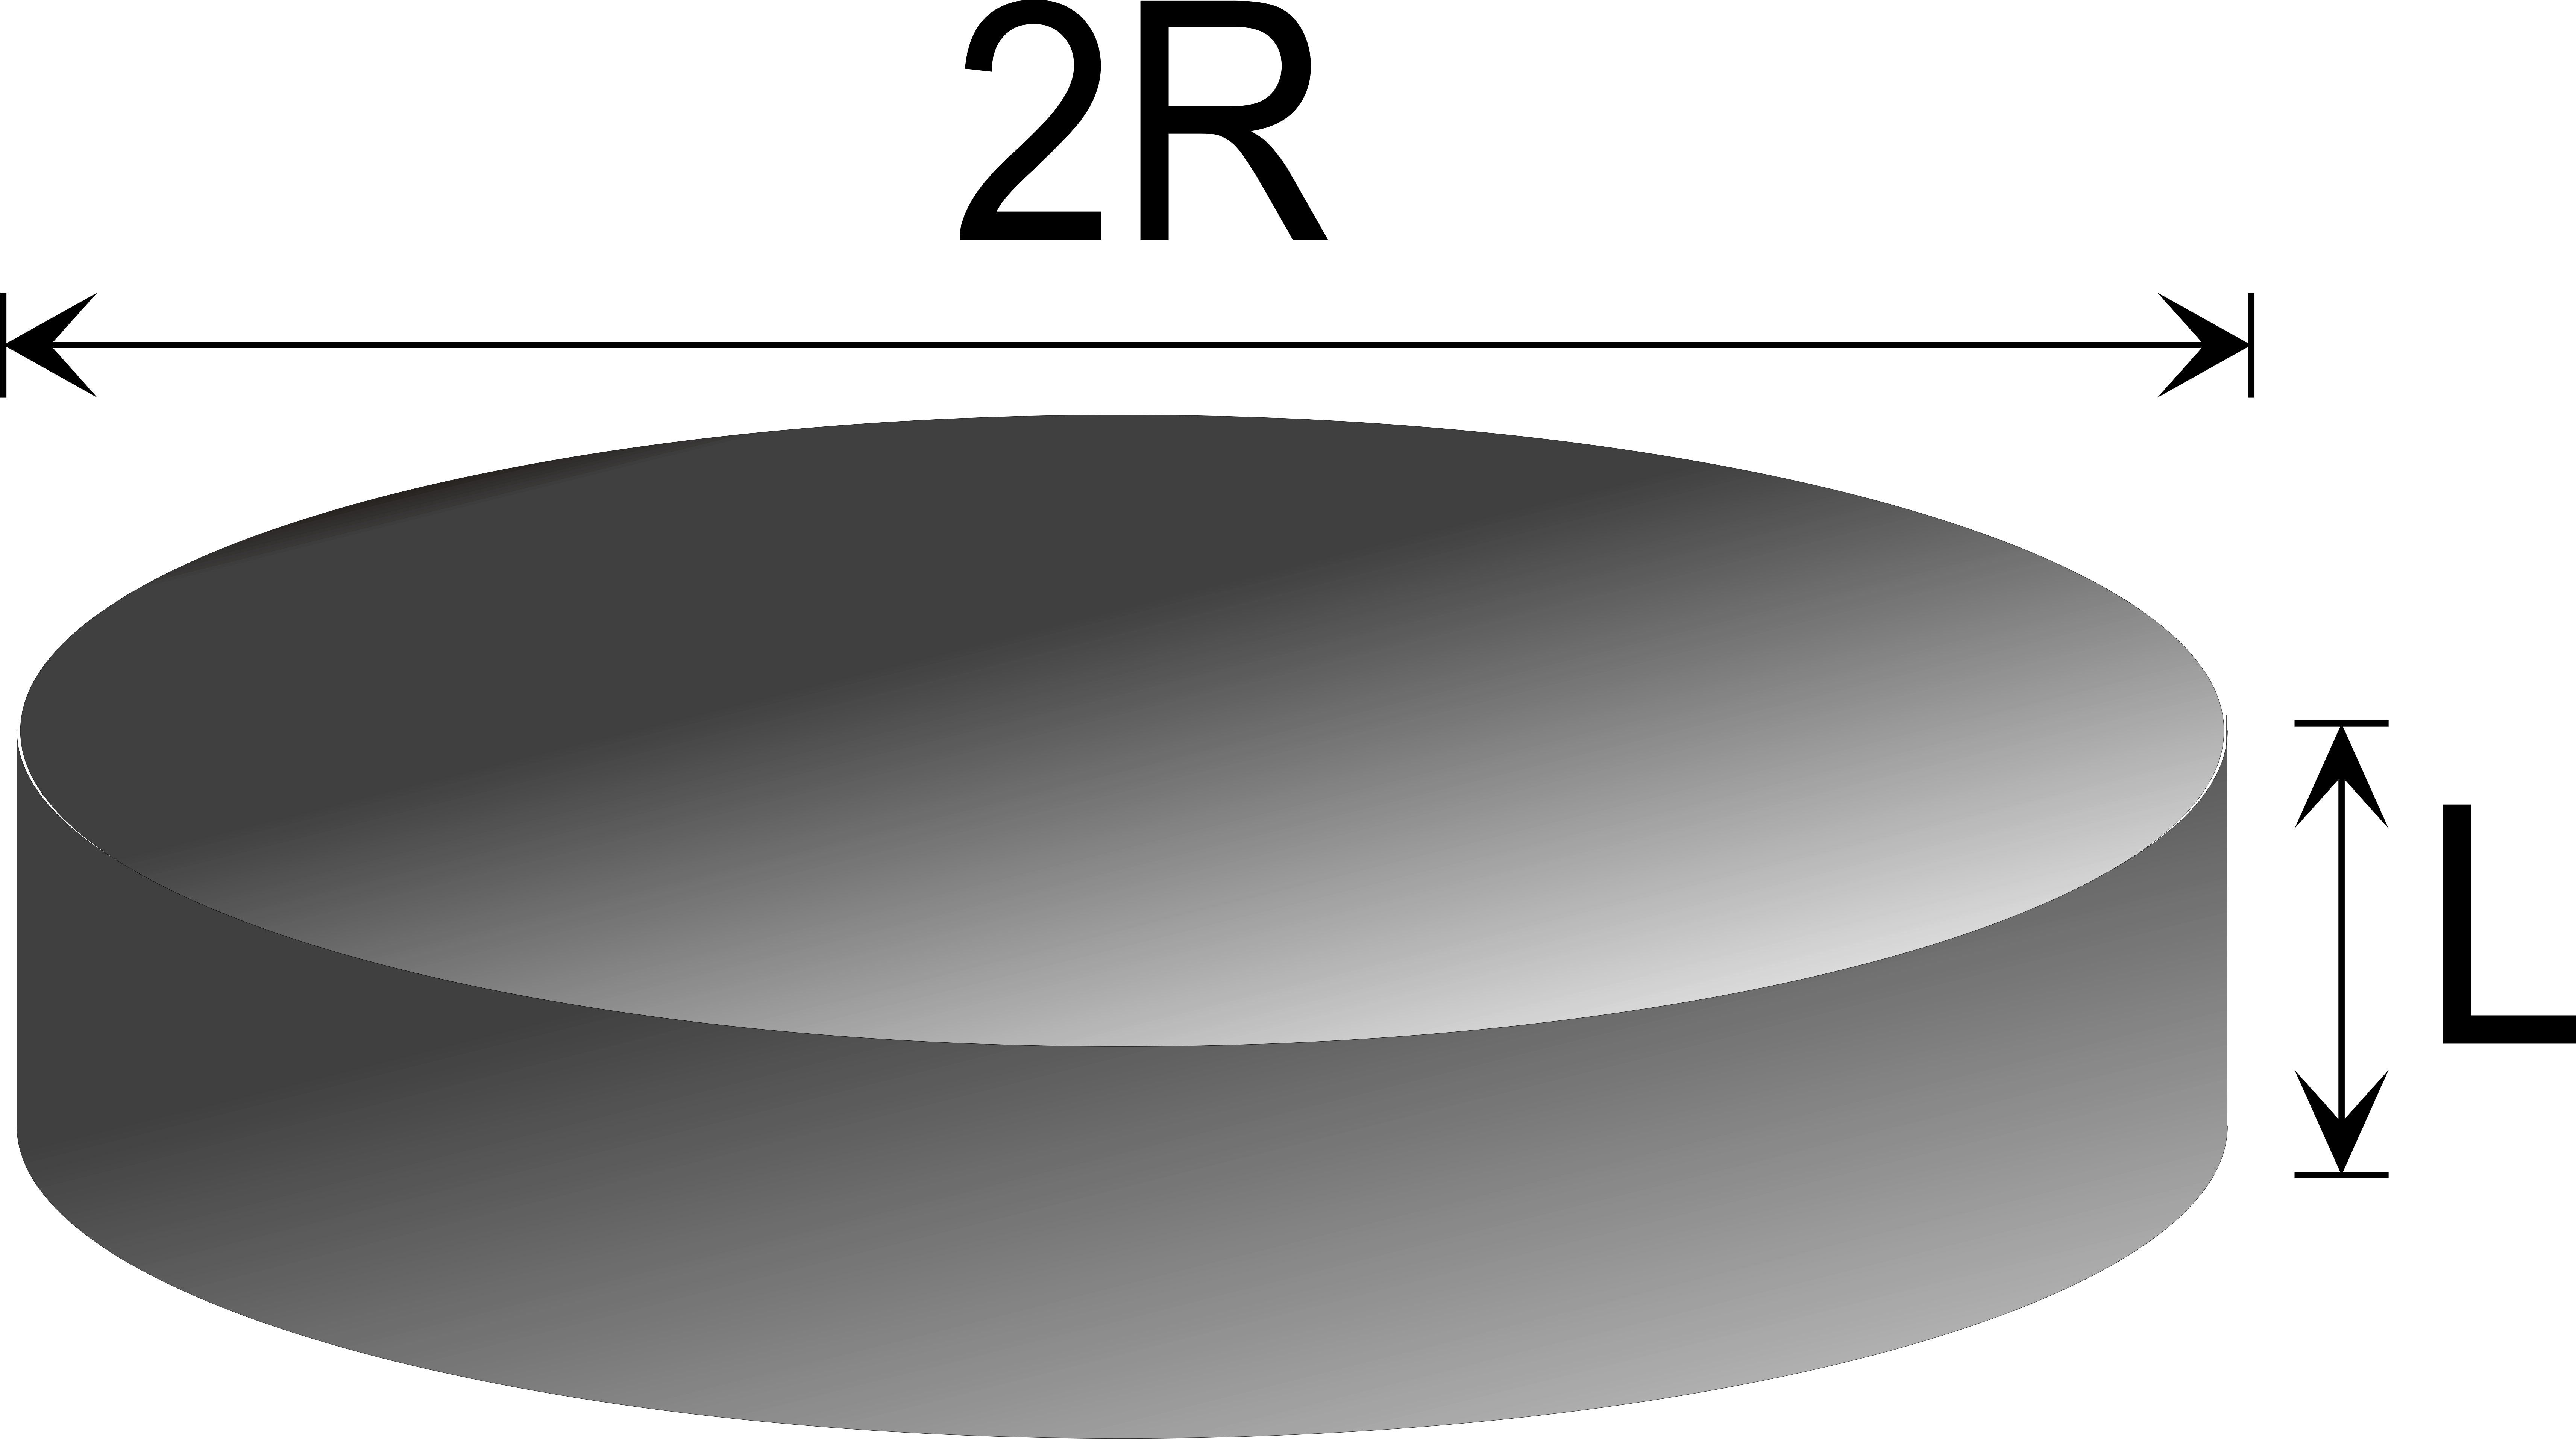
\includegraphics[width=0.7\textwidth,height=0.42\textwidth]{../images/form_factor/cylindrical_obj/flat_cylinder.png}
\end{center}
\caption{} \label{flatcylinder}
\end{figure}

\begin{align}
\Lambda_1(x) &= \frac{2}{x} J_1(x) \\
I_1(x) &= \int\limits_0^x \Lambda_1(x') dx' = \\
& \quad 2x \mathrm{J}_0(x)-2\mathrm{J}_1(x)+\pi x \left[J_0(x)\mathrm{H}_1(x)-\mathrm{J}_1(x)\mathrm{H}_0(x)\right] \nonumber \\
I_0(x) &= \frac{I_1(x)+x\Lambda_1(x)}{2}\\
\Omega(x) &= \frac{2}{x} \left[ I_0(x)-2\mathrm{J}_1(x)\right]\\
\chi(x) &= \left( \frac{\sin(x/2)}{x/2}\right)^2\\
\Phi_\text{flat}(q,R,L) &= \left(\Delta\eta\pi R^2L\right)^2 \frac{8}{(2qR)^2}  \label{eq:FlatCylinder}\\
& \quad \times \left\{ \chi(qL) +
\frac{I_1(2QR)\;\Omega(qL)}{2qR}-\Lambda_1(2qR)\right\}\nonumber
\end{align}
$\mathrm{H}_\alpha(x)$ is the Struve function of order $\alpha$ and $\mathrm{J}_n(x)$ are the regular cylindrical Bessel function of order $n$.

\vspace{5mm}

\underline{Input Parameters for model \texttt{FlatCylinder}:}
\begin{description}
\item[\texttt{R}] radius of cylinder $R$
\item[\texttt{L}] length of cylinder $L$
\item[\texttt{eta}] scattering contrast $\Delta\eta$
\end{description}

\underline{Note:}
\begin{itemize}
\item The approximation is valid for $L<2R$
\end{itemize}

\begin{figure}[htb]
\begin{center}
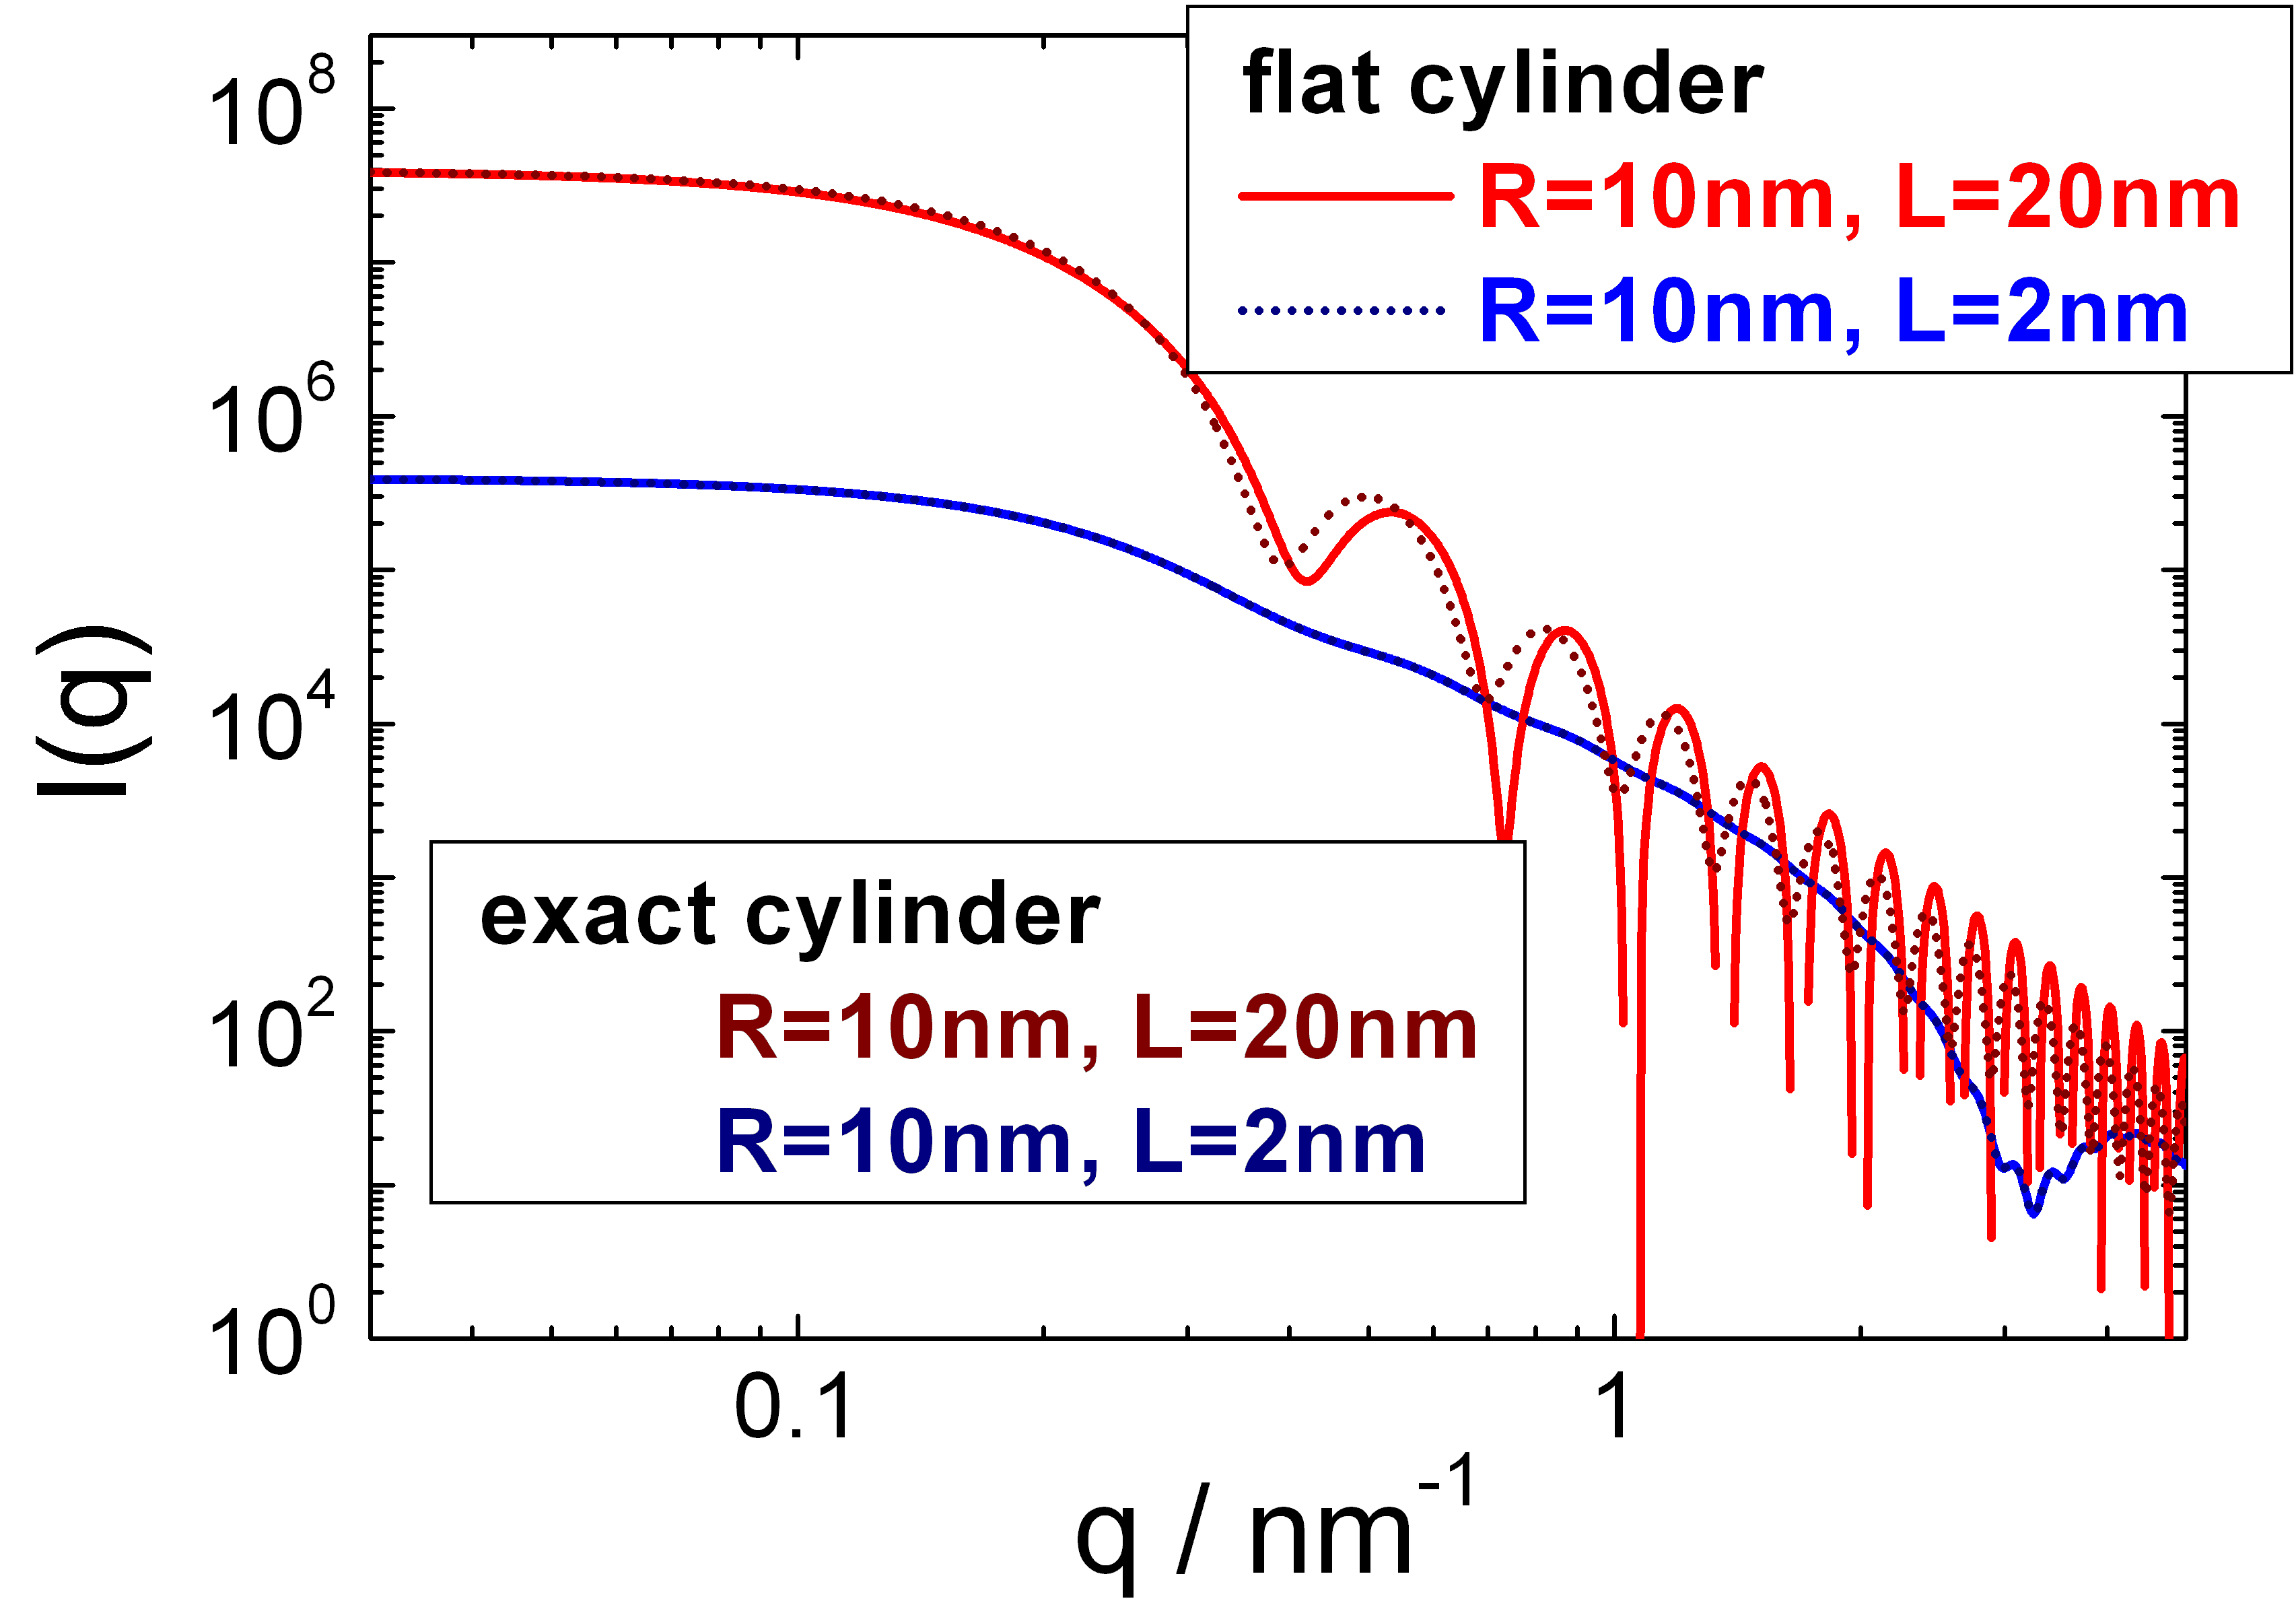
\includegraphics[width=0.668\textwidth,height=0.488\textwidth]{../images/form_factor/cylindrical_obj/FlatCylinder.png}
\end{center}
\caption{Scattering intensity of a cylinder with radius $R=10$ nm and lengths of $L=2$ nm
and $L=20$ nm. Next to Porod's axproximation for flat cylinders also
the exact integral solution is shown for comparison.
The scattering length density contrast is set to 1.}
\label{fig:FlatCylinder}
\end{figure}

\clearpage

\subsection{Porod's approximations for cylinder \cite{Porod1948}}
\label{sect:PorodCylinder}
~\\
\begin{figure}[htb]
\begin{center}
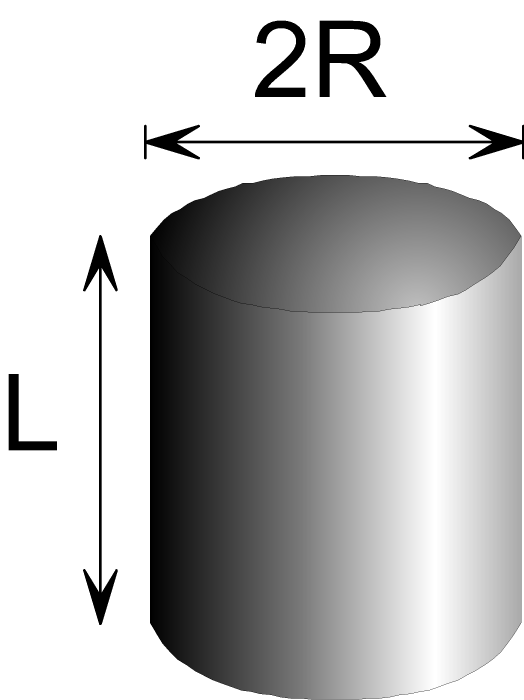
\includegraphics[width=0.288\textwidth,height=0.385\textwidth]{../images/form_factor/cylindrical_obj/cylinder.png}
\end{center}
\caption{} \label{PorodCylinder}
\end{figure}

This form factor combines the two solutions of Porod for a long $\Phi_\text{long}(q,R,L)$
(\ref{eq:LongCylinder}) and a flat $\Phi_\text{flat}(q,R,L)$ (\ref{eq:FlatCylinder}) cylinder
by a linear combination of both. A simple linear transition at $L=2R$ is assumed.
\begin{align}
\Phi_\text{Porod}(q,R,L) &= p\left(\frac{2R}{L}\right)\Phi_\text{flat}(q,R,L) + \left(1-p\left(\frac{2R}{L}\right)\right)\Phi_\text{long}(q,R,L) \\
p(x) &=
\begin{cases}
    1 & \mbox{for } x > \frac54 \\
    2\left(x-\frac34\right) & \mbox{for }\frac34 \leq x \leq \frac54 \\
    0 & \mbox{for } x < \frac34
\end{cases}
\end{align}

\vspace{5mm}

\underline{Input Parameters for model \texttt{PorodCylinder}:}
\begin{description}
\item[\texttt{R}] radius of cylinder $R$
\item[\texttt{L}] length of cylinder $L$
\item[\texttt{eta}] scattering contrast $\Delta\eta$
\end{description}

\underline{Note:}
\begin{itemize}
\item less good approximation  for $L \sim 2R$
\end{itemize}

\begin{figure}[htb]
\begin{center}
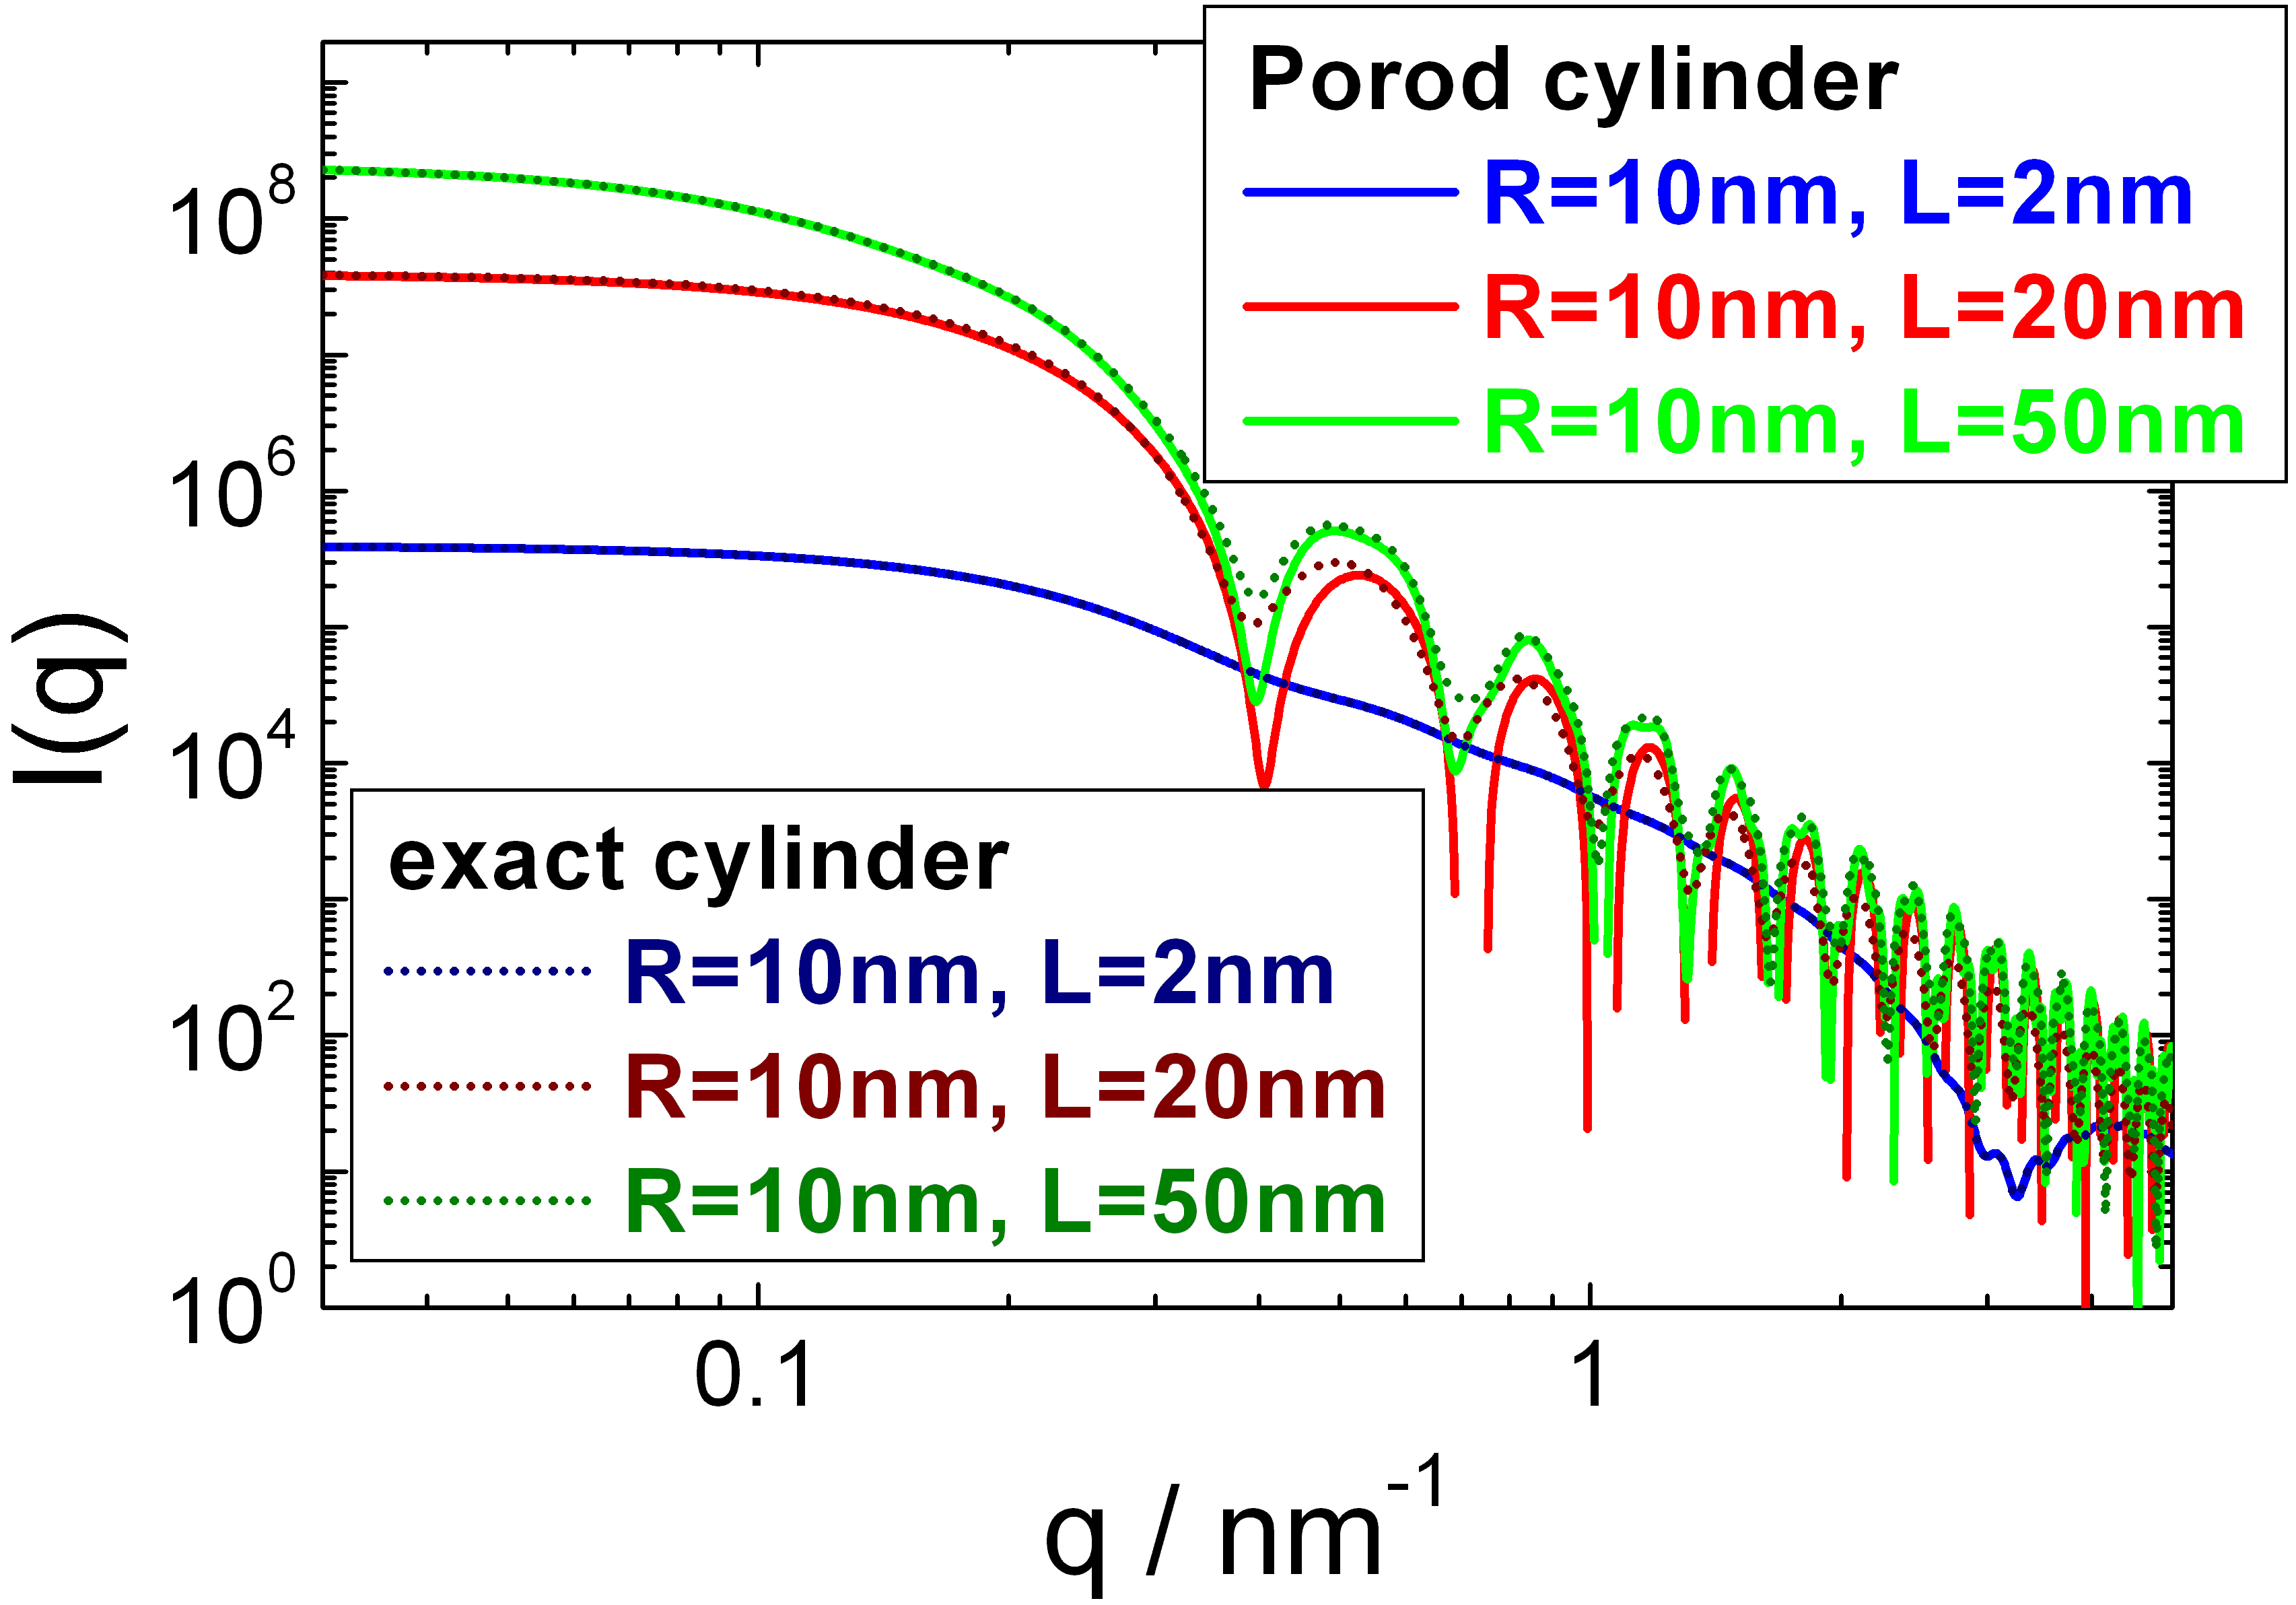
\includegraphics[width=0.55\textwidth,height=0.4\textwidth]{../images/form_factor/cylindrical_obj/PorodCylinder.png}
\end{center}
\caption{Scattering intensity of a cylinder with radius $R=10$ nm and lengths of $L=2$ nm,
$L=20$ nm, and $L=50$ nm. Next to Porod's axproximation for a cylinders also
the exact integral solution is shown for comparison.
The scattering length density contrast is set to 1.}
\label{fig:PorodCylinder}
\end{figure}
%%%%%%%%%%%%%%%%%%%%%%%%%%%%%%%%%%%%%%%%%%%%%%%%%%%%%%%%%%%%%%%%%%%%%%%%%%

\clearpage
\subsection{Cylinder of length $L$, radius $R$ and scattering
contrast $\Delta\eta$}
\label{sect:Cylinder}
~\\

\begin{figure}[htb]
\begin{center}
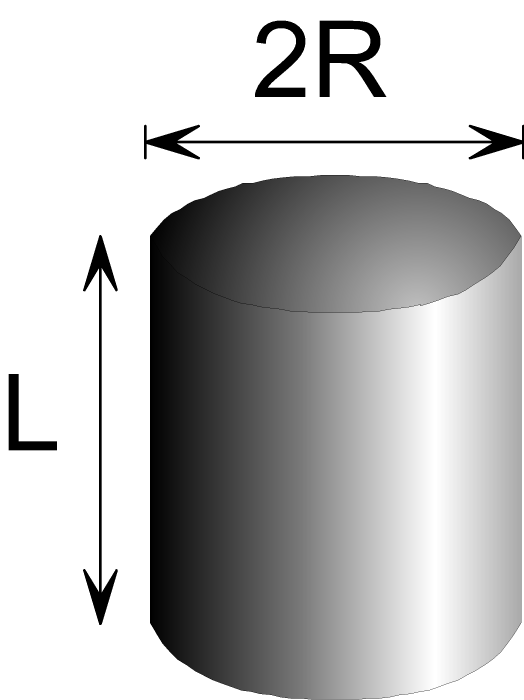
\includegraphics[width=0.192\textwidth,height=0.257\textwidth]{../images/form_factor/cylindrical_obj/cylinder.png}
\end{center}
\caption{} \label{fig:cylinder}
\end{figure}
\begin{align}
I_\text{cyl} = 16 (\pi R^2 L)^2 \Delta\eta^2 \int_0^1 \left(
\frac{J_1\left(Q R \sqrt{1-x^2}\right)
                         \sin(Q L x/2)}{Q^2 R \sqrt{1-x^2} L x}
                      \right)^2 dx
\end{align}
\vspace{5mm}

\underline{Input Parameters for model \texttt{Cylinder}:}
\begin{description}
\item[\texttt{R}] radius of cylinder $R$
\item[\texttt{L}] length of cylinder $L$
\item[\texttt{eta}] scattering contrast $\Delta\eta$
\end{description}

\underline{Note:}
\begin{itemize}
\item None
\end{itemize}

\begin{figure}[htb]
\begin{center}
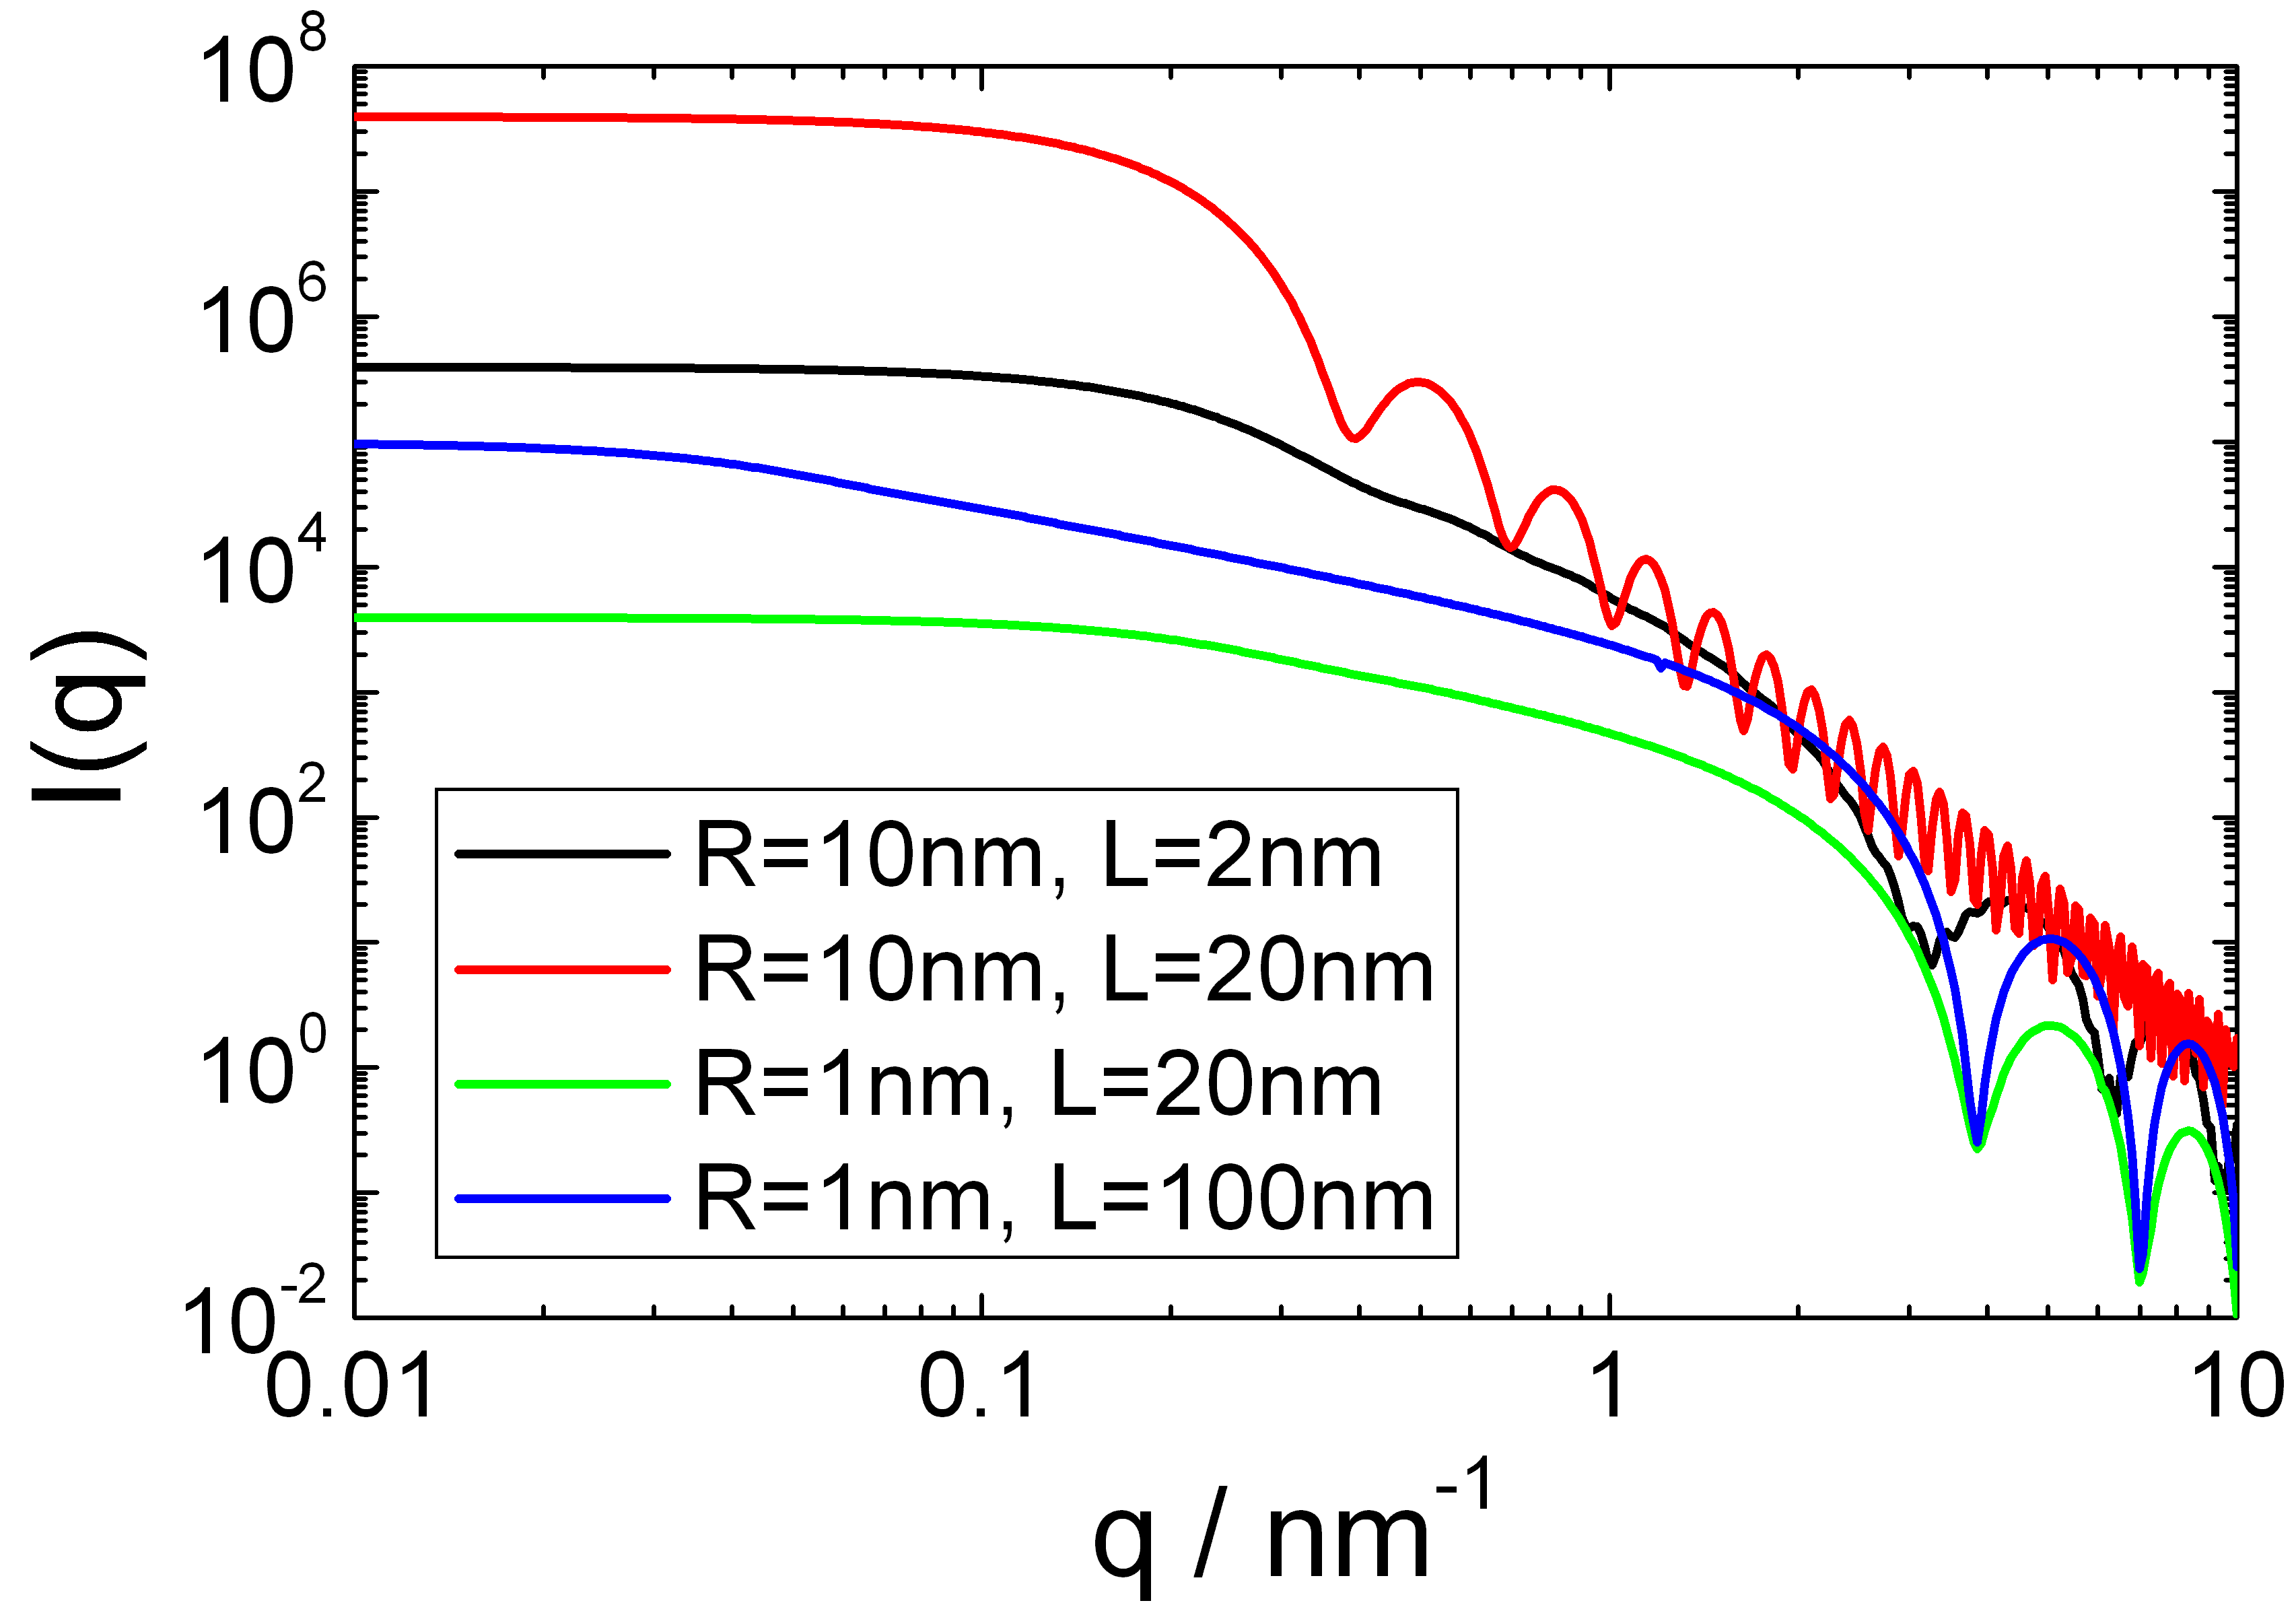
\includegraphics[width=0.55\textwidth,height=0.4\textwidth]{../images/form_factor/cylindrical_obj/ExactCylinder.png}
\end{center}
\caption{Scattering intensity of a cylinder for different radii radius $R$ nm and lengths $L$.
The scattering length density contrast is set to 1.}
\label{fig:ExactCylinder}
\end{figure}

%%%%%%%%%%%%%%%%%%%%%%%%%%%%%%%%%%%%%%%%%%%%%%%%%%%%%%%%%%%%%%%%%%%%%%%%%%

\clearpage
\subsection{Random oriented cylindrical shell with circular cross-section}
\label{sect:randomCylindricalShell}
~\\

\begin{figure}[htb]
\begin{center}
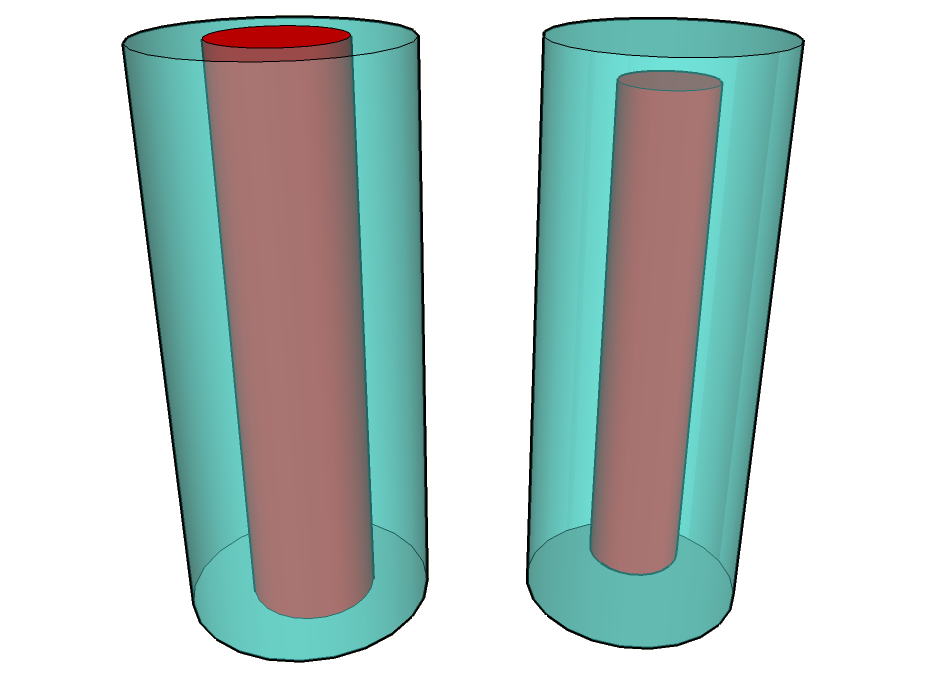
\includegraphics[width=0.4\textwidth,height=.293\textwidth]{../images/form_factor/cylindrical_obj/CylShell.png}
\hspace{0.1\textwidth}
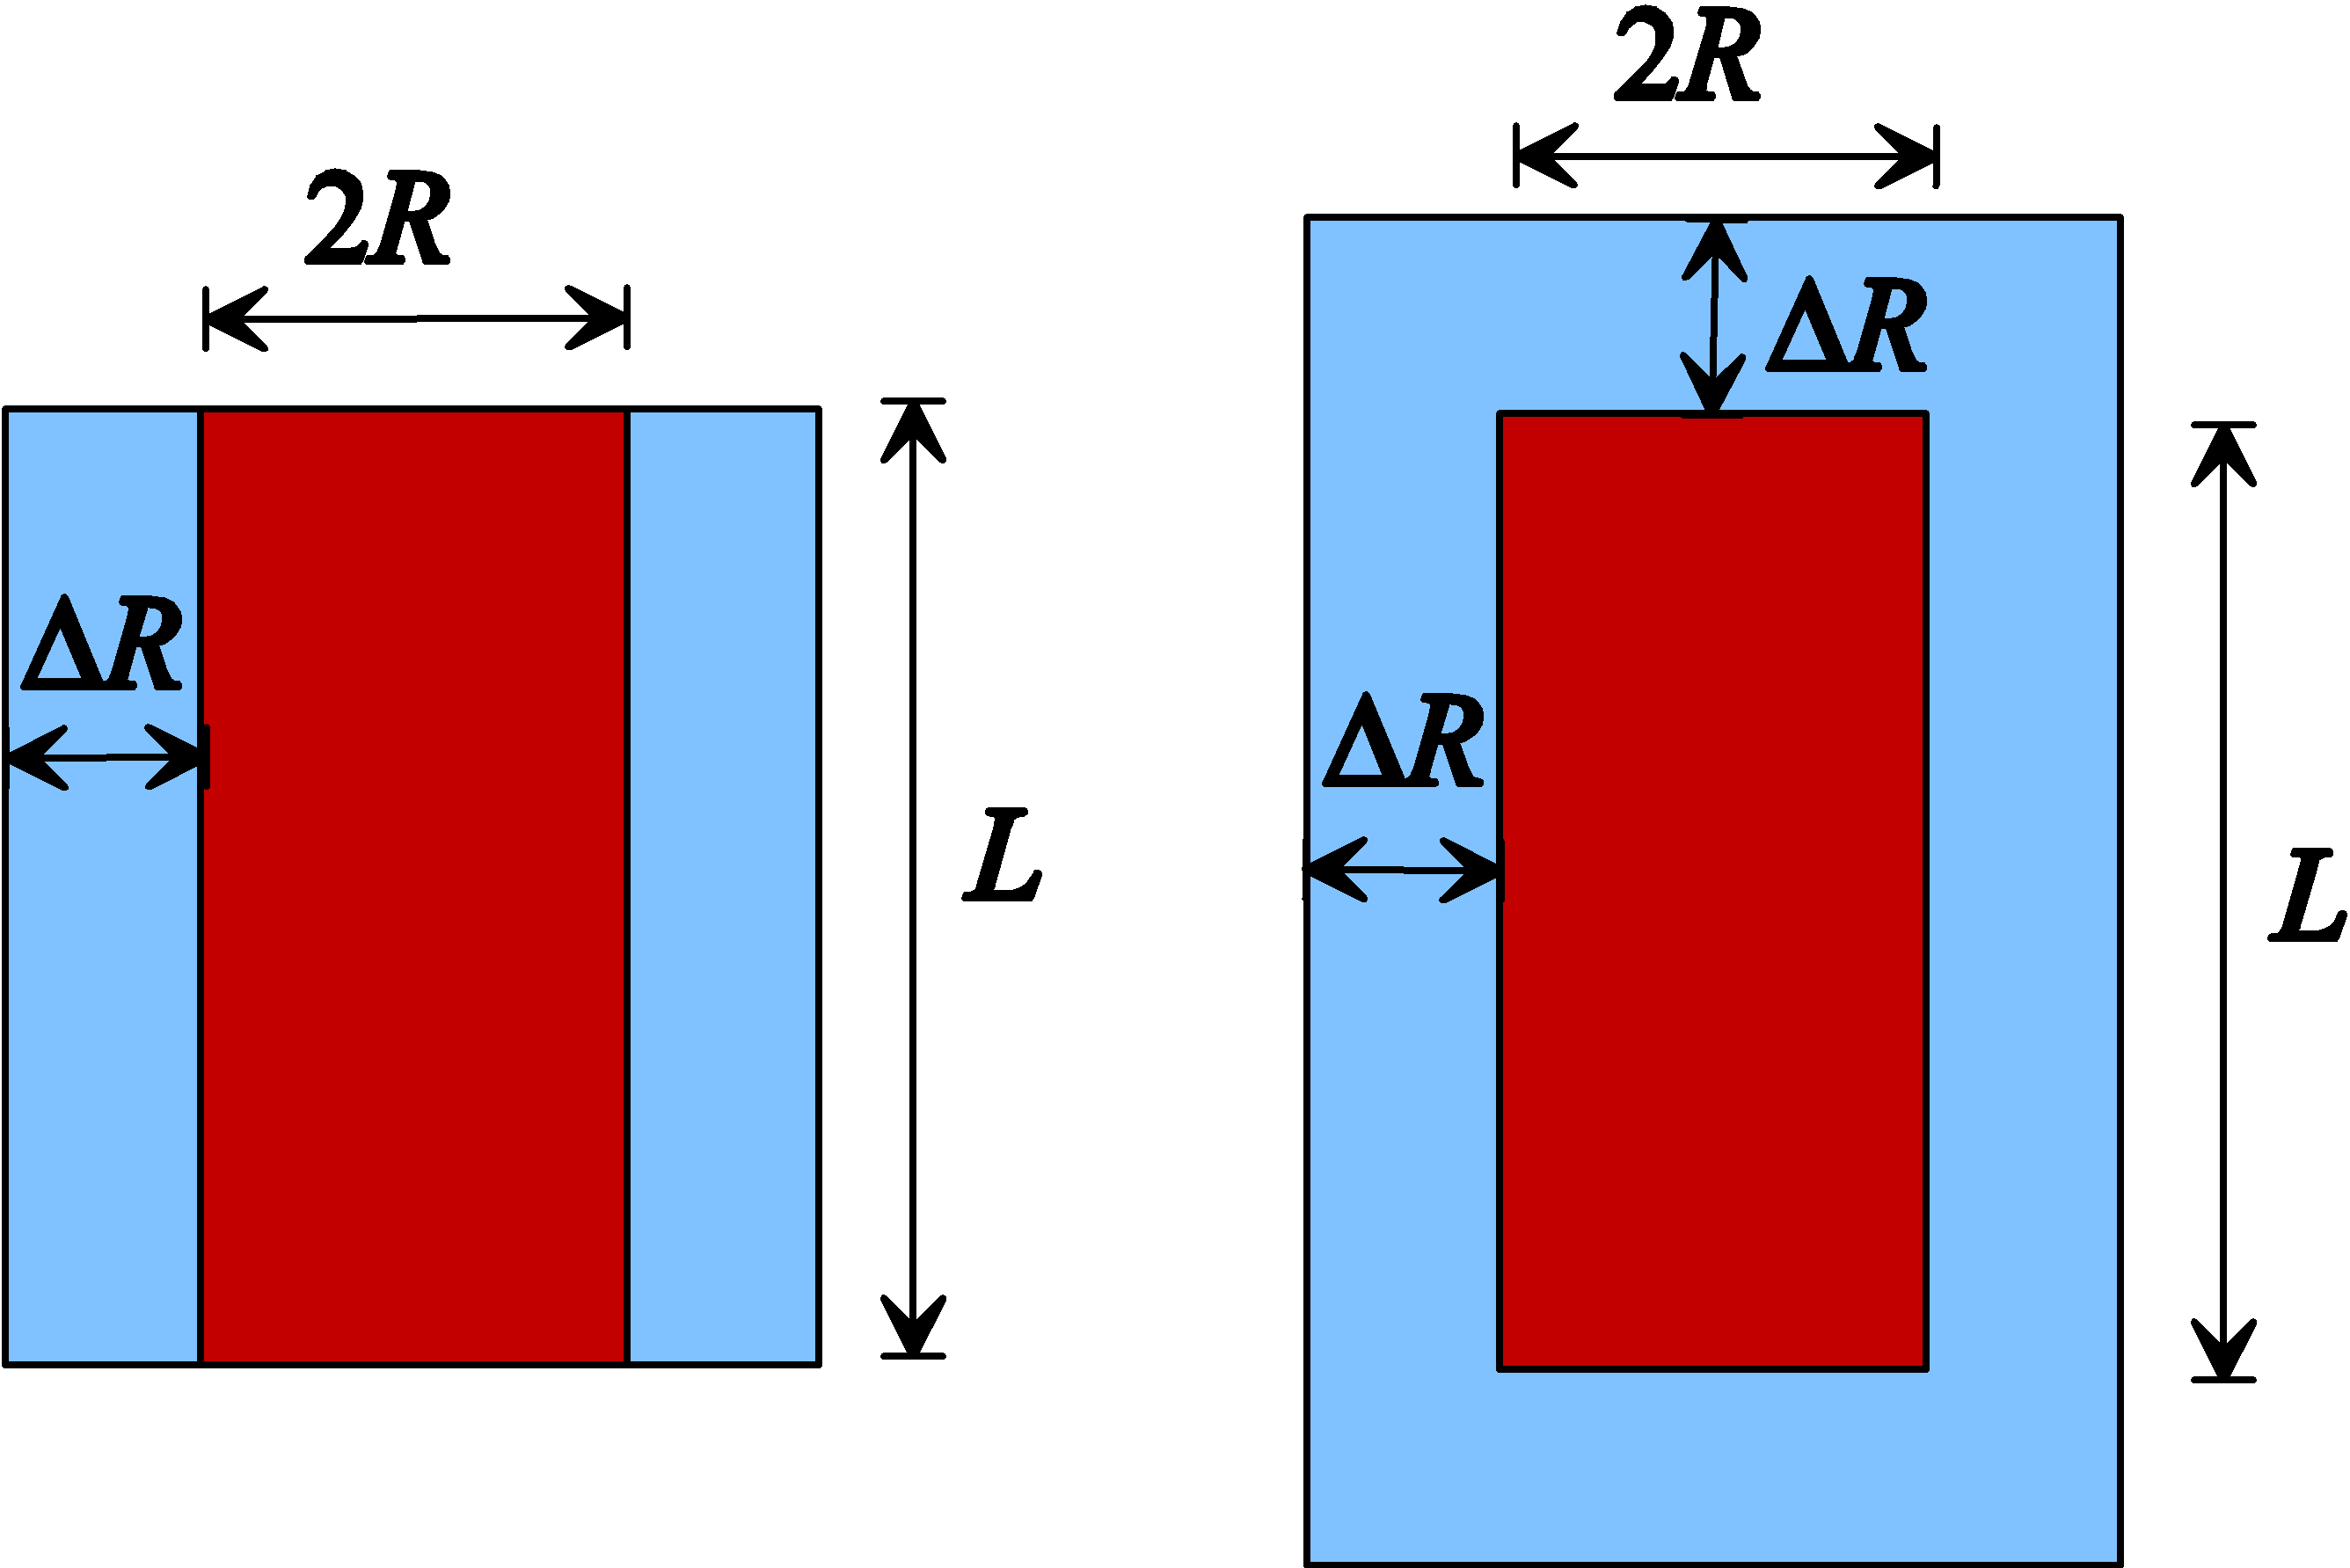
\includegraphics[width=.4\textwidth,height=0.27\textwidth]{../images/form_factor/cylindrical_obj/cylshell2D.png}
\end{center}
\caption{cylindrical shell with circular cross-section}
\label{cylshell}
\end{figure}

To different versions for a random oriented cylindrical shell with a
circular cross-section has been implemented. One without  \texttt{CylShell1}
and one with \texttt{CylShell2} capped ends. For very long cylinders a faster
approximation for the uncapped version can be used \texttt{LongCylShell}

\begin{align}
K_\text{Cyl}(Q,\Delta\eta,R,L,x) =
2 \pi R^2 L \Delta \eta
    \frac{J_1\left(Q R \sqrt{1-x^2}\right)}{Q R \sqrt{1-x^2}}
    \frac{\sin(Q L x/2)}{QL x/2}
\end{align}

\begin{align}
I_\text{CylShell1} =
\int_0^1 \biggl(
  &
  K_\text{Cyl}\left(Q,\eta_\text{core}-\eta_\text{shell},R,L,x\right) \\
+&  K_\text{Cyl}\left(Q,\eta_\text{shell}-\eta_\text{solv},R+\Delta R,L,x\right)
\biggr)^2 dx \nonumber \\
I_\text{CylShell2} =
\int_0^1 \biggl(
 &  K_\text{Cyl}\left(Q,\eta_\text{core}-\eta_\text{shell},R,L,x\right) \\
+&  K_\text{Cyl}\left(Q,\eta_\text{shell}-\eta_\text{solv},R+\Delta R,L+2\Delta R,x\right)
\biggr)^2 dx \nonumber
\end{align}

\begin{align}
  I_\text{LongCylShell}(Q) = & P'(Q) P_\text{cs}(Q) \\
  P'(Q)  = & 2 \frac{\text{Si}(Q L)}{QL} - \left(\frac{\sin(QL/2)}{QL/2}\right) \\
  \text{Si}(x) & = \int_0^x\!\frac{\sin t}{t}\,\,dt \\
  P_\text{cs}(Q)  =  & \biggl(
            2\frac{J_1(QR)}{QR}
            \left(\eta_\text{core}-\eta_\text{shell}\right)R^2L\pi + \\
         & \qquad
            2\frac{J_1(Q(R+\Delta R))}{Q(R+\Delta R)}
            \left(\eta_\text{shell}-\eta_\text{solv}\right)(R+\Delta R)^2L\pi
      \biggr)^2  \nonumber
\end{align}


\vspace{5mm}

\hspace{1pt}\\
\underline{Input Parameters for models \texttt{CylShell1}, \texttt{CylShell2} and \texttt{LongCylShell}:}\\
\begin{description}
\item[\texttt{R}] core radius $R$
\item[\texttt{DR}] shell thickness $\Delta R$
\item[\texttt{L}] cylinder length $L$
\item[\texttt{eta\_core}] scattering length density $\eta_\text{core}$ of cylinder core
\item[\texttt{eta\_shell}] scattering length density $\eta_\text{shell}$ of cylinder shell
\item[\texttt{eta\_solv}] scattering length density $\eta_\text{solv}$ of solvent
\end{description}

\underline{Note:}
\begin{itemize}
\item The approximation for a long cylindrical shell (\texttt{LongCylShell}) only holds for $L \gg 2R$.
\end{itemize}

\begin{figure}[htb]
\begin{center}
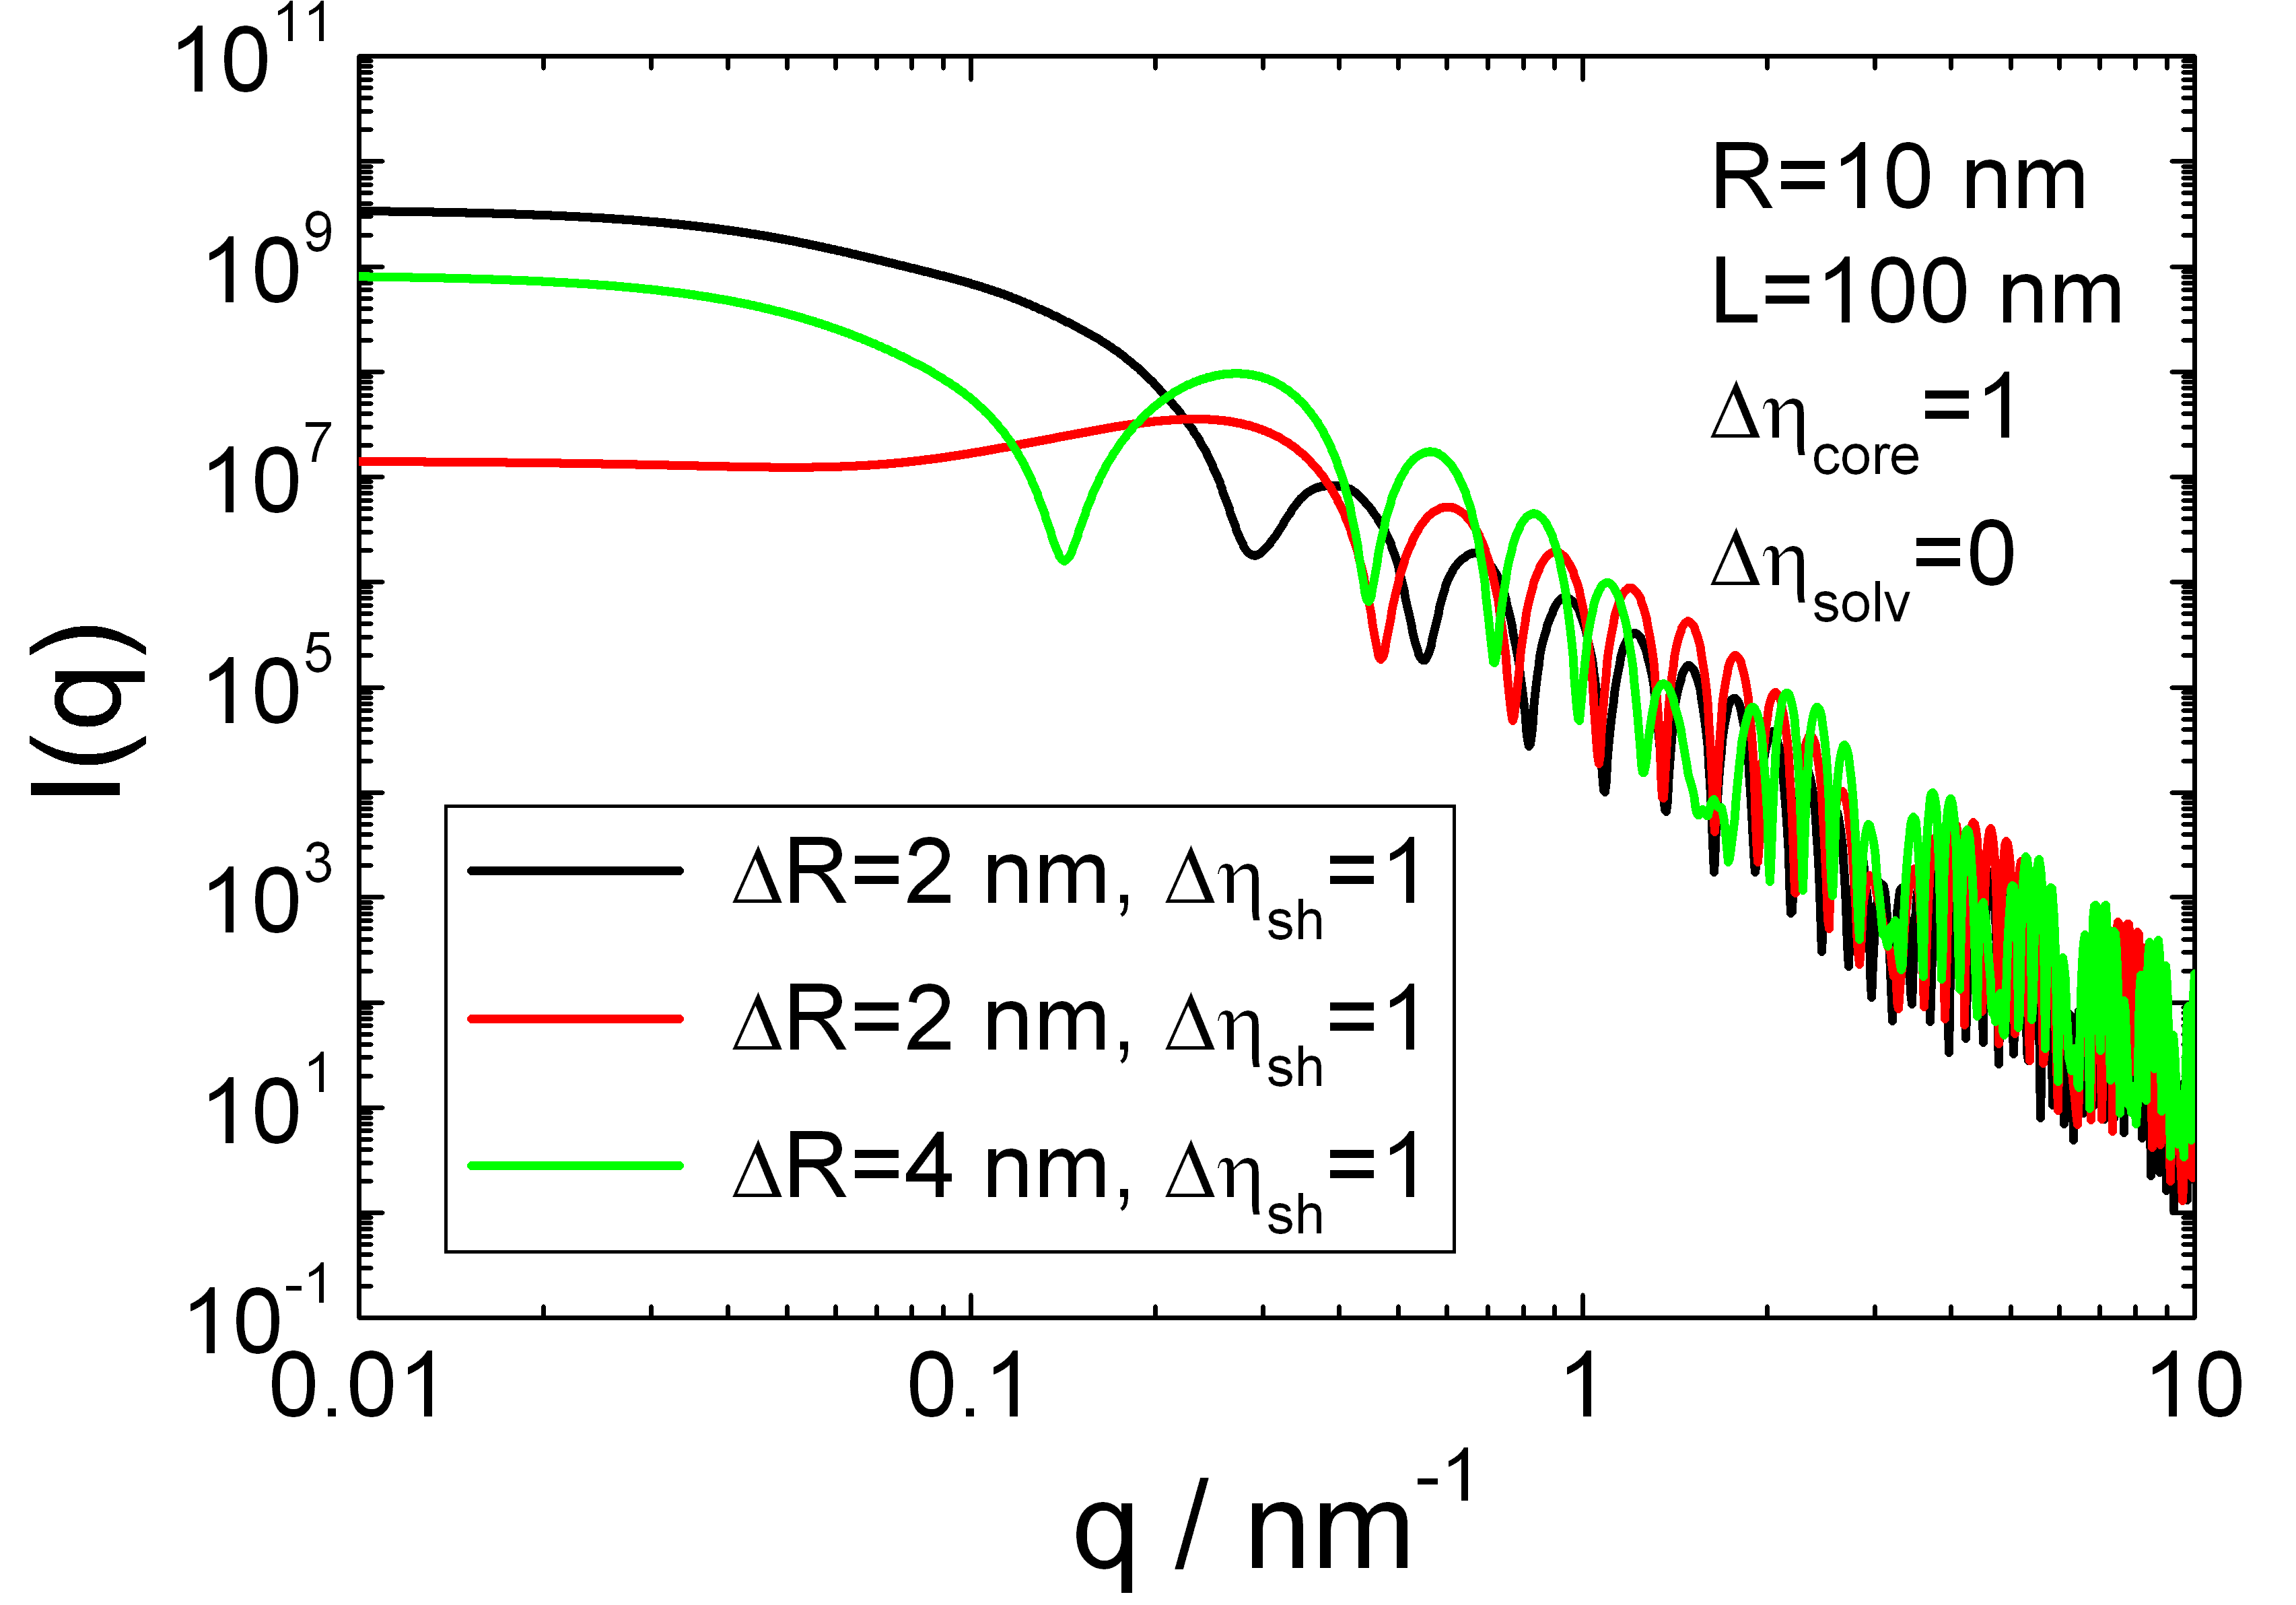
\includegraphics[width=0.55\textwidth,height=0.4\textwidth]{../images/form_factor/cylindrical_obj/CylShell1IQ.png}
\end{center}
\caption{Scattering intensity of a cylinder shell \texttt{CylShell1}.}
\label{fig:CylShell1}
\end{figure}

\begin{figure}[htb]
\begin{center}
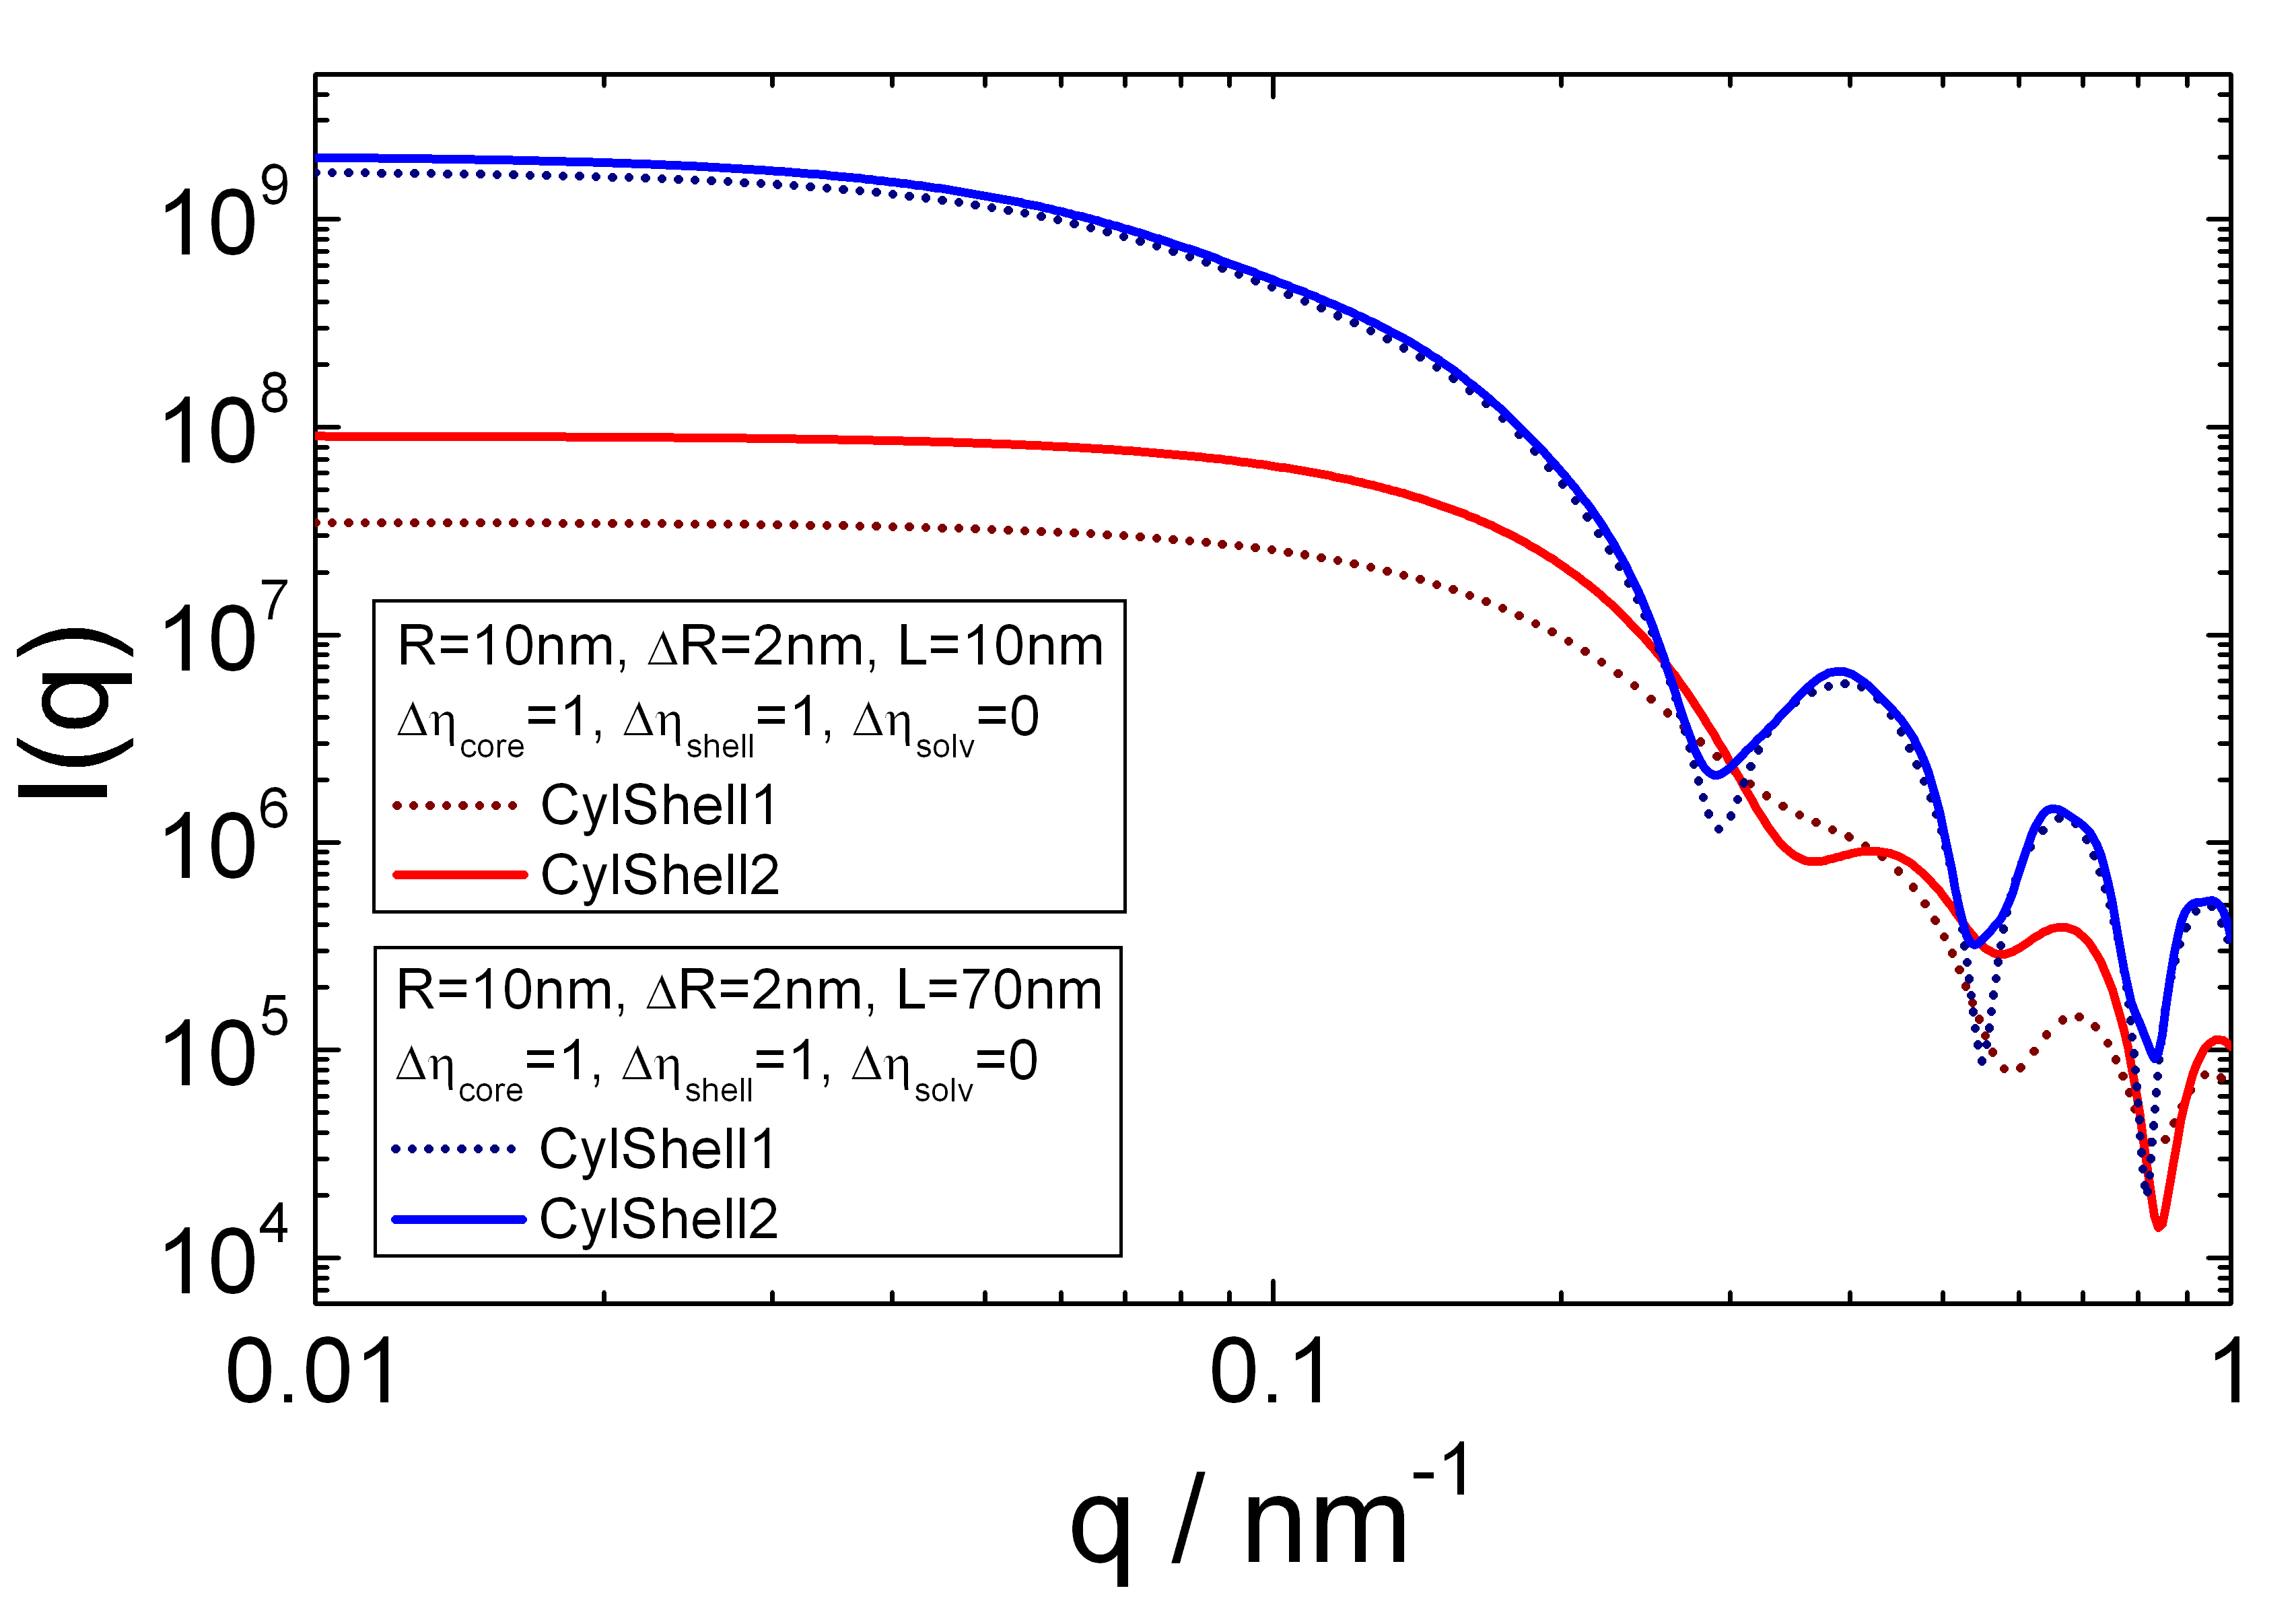
\includegraphics[width=0.55\textwidth,height=0.4\textwidth]{../images/form_factor/cylindrical_obj/CylShell2IQ.png}
\end{center}
\caption{Scattering intensity of a cylinder shell \texttt{CylShell2}.}
\label{fig:CylShell2}
\end{figure}


%%%%%%%%%%%%%%%%%%%%%%%%%%%%%%%%%%%%%%%%%%%%%%%%%%%%%%%%%%%%%%%%%%%%%%%%%%%%%%%%%%%%%%%%%%%%

\clearpage
\subsection{Random oriented cylindrical shell with elliptical cross-section}
\label{sect:random_ellCylinderShell}
~\\

\begin{figure}[htb]
\begin{center}
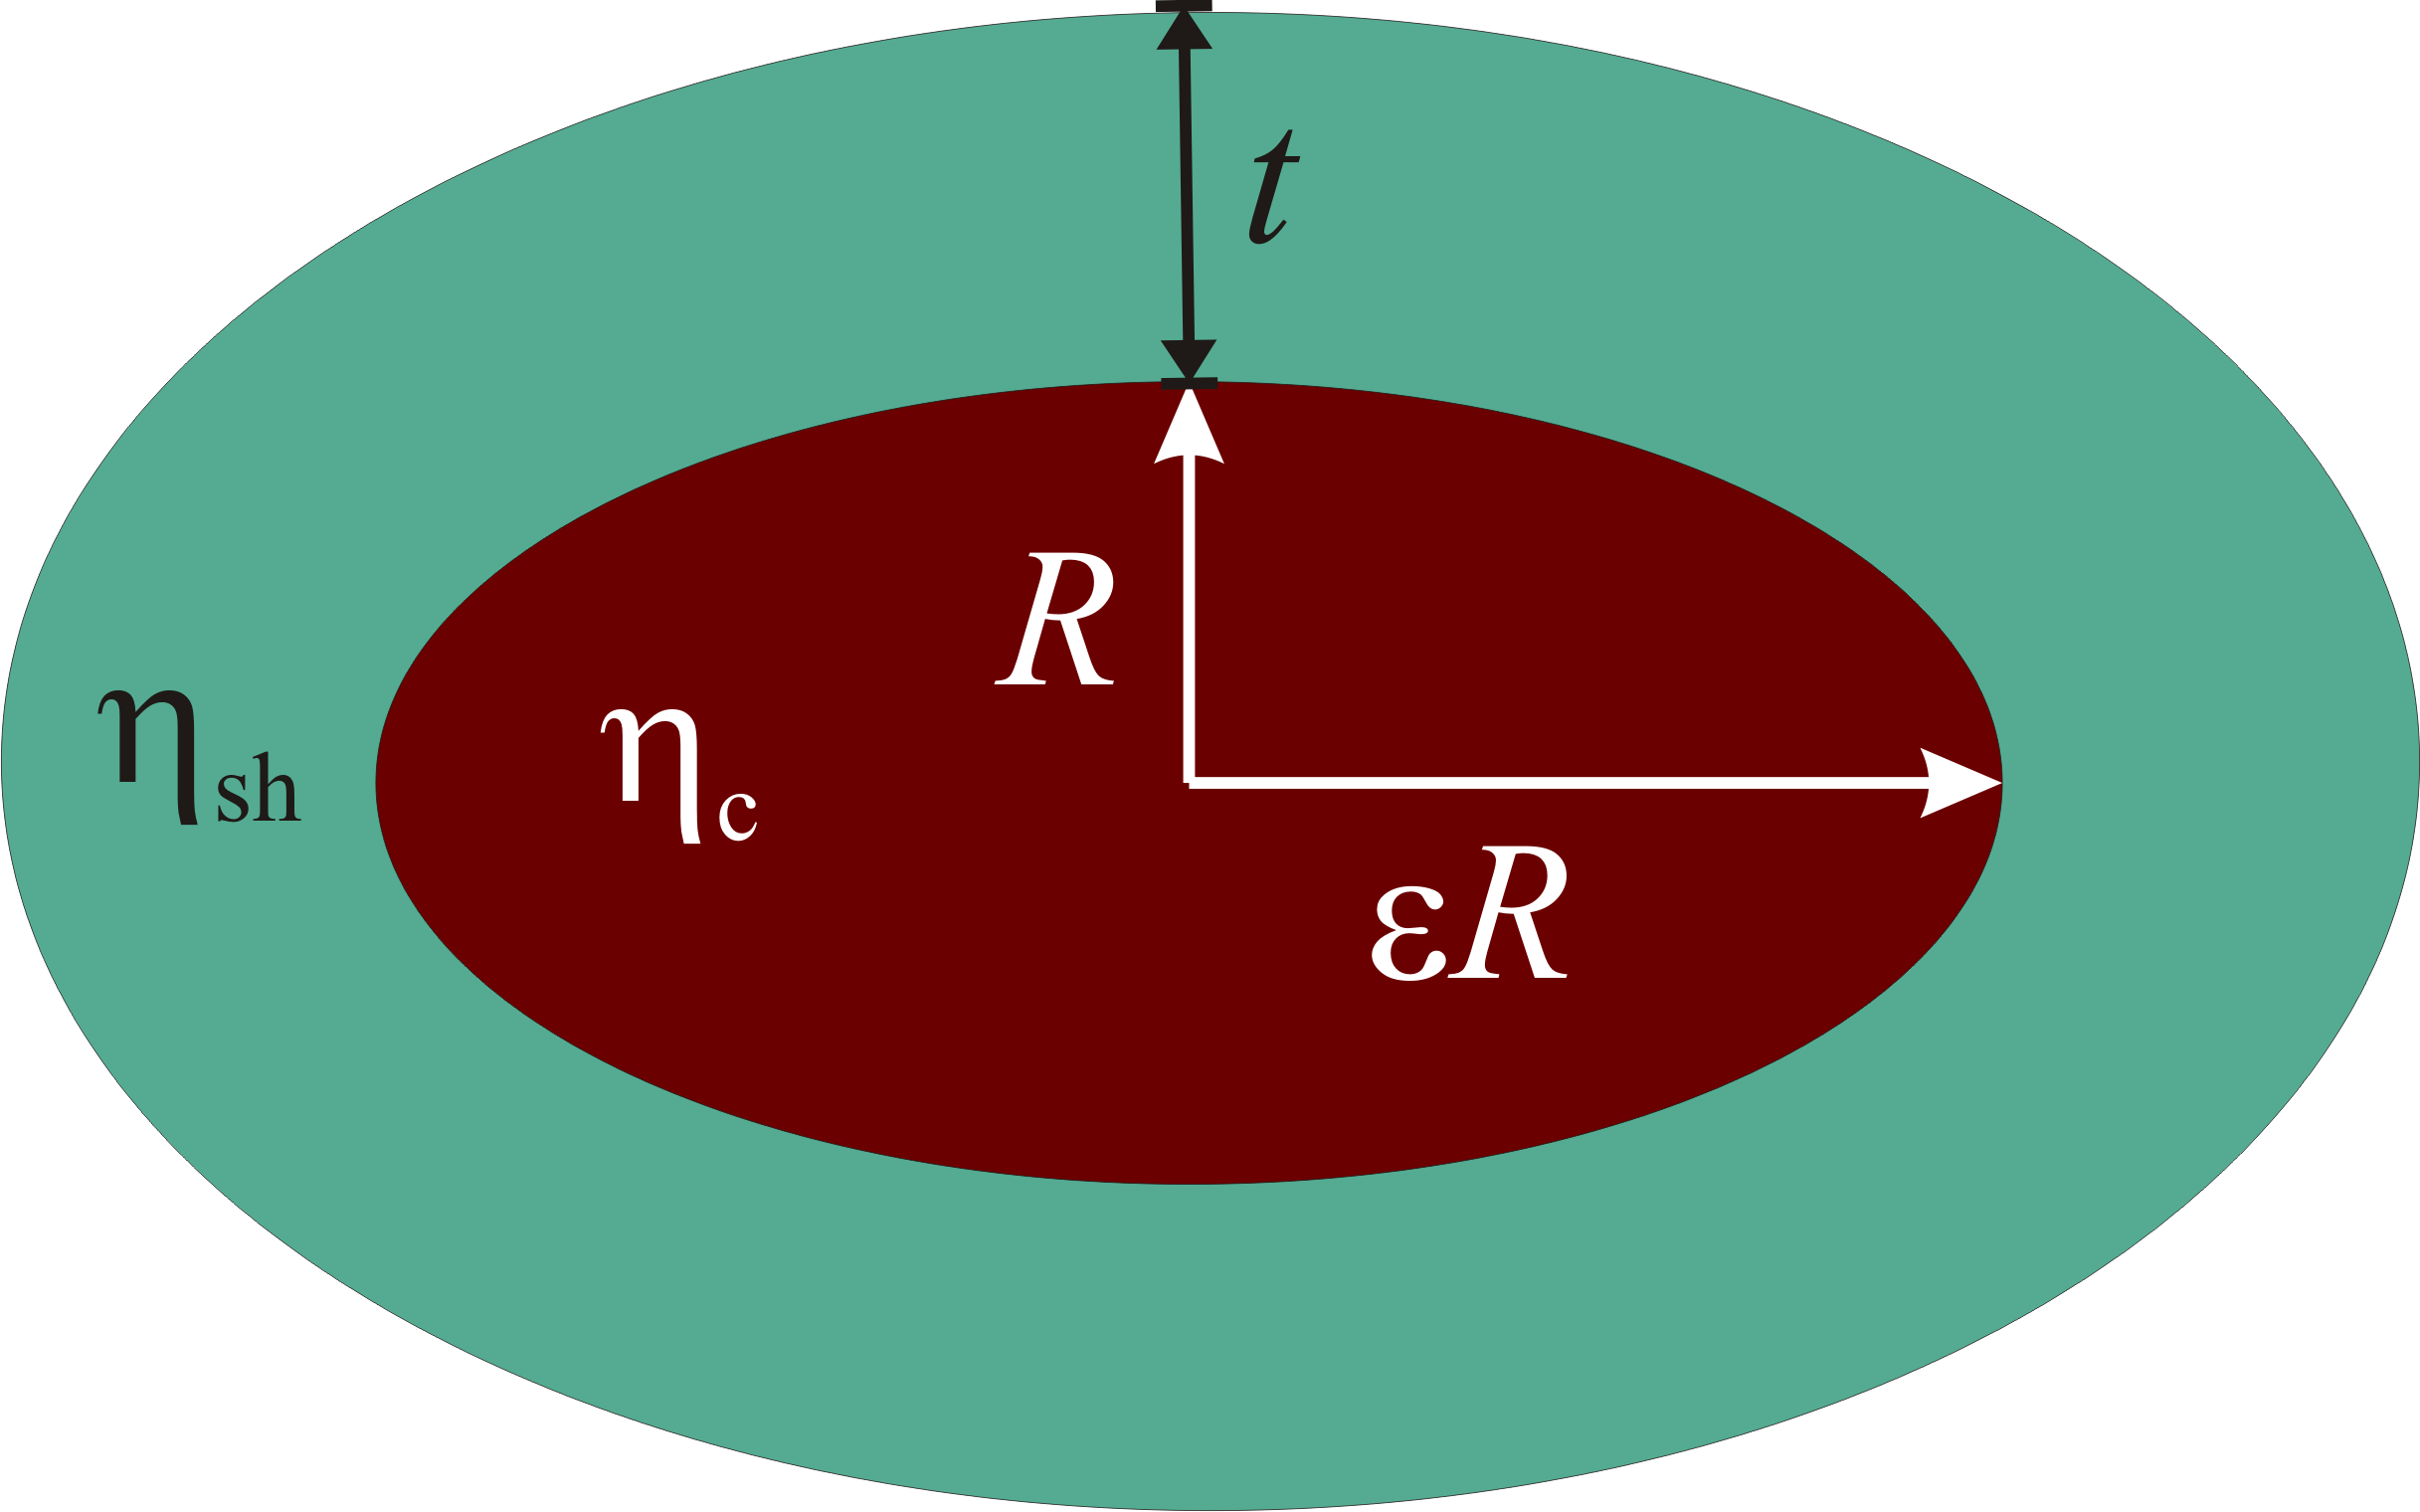
\includegraphics[width=0.4866\textwidth,height=.304\textwidth]{../images/form_factor/cylindrical_obj/ellCylShell_shape.png}
\hspace{0.0\textwidth}
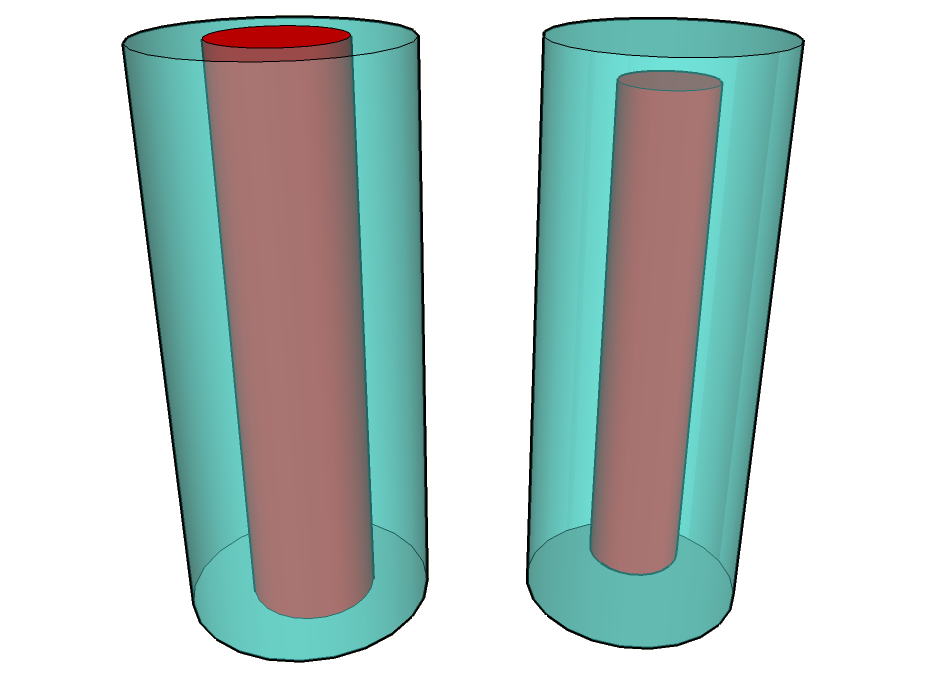
\includegraphics[width=0.4\textwidth,height=.293\textwidth]{../images/form_factor/cylindrical_obj/CylShell.png}
\end{center}
\caption{cylindrical shell with elliptical cross-section}
\label{fig:ellCylShell}
\end{figure}

To different versions for a random oriented cylindrical shell with
an elliptical cross-section has been implemented. One without
\texttt{ellCylShell1} and one with \texttt{ellCylShell2} capped
ends.

\begin{align}
K_\text{ellCyl}(q,\Delta\eta,R,\epsilon,L,t,\phi,\alpha) &= \pi \epsilon R(\epsilon R+t) L
\Delta \eta \\
    & \times \frac{2J_1\left(q r(R,\epsilon,\phi,\alpha) \right)}{q r(R,\epsilon,\phi,\alpha)}
    \frac{\sin(q \frac{L}{2}\cos(\alpha))}{q\frac{L}{2}\cos(\alpha)} \nonumber \\
r(R,\epsilon,t,\phi,\alpha) &= \sqrt{R^2\sin^2(\phi)+(\epsilon R+t)^2\cos^2(\phi)} \sin(\alpha)
\end{align}

\begin{align}
I_\text{ellCylShell1}(q) = \frac{2}{\pi}\int_0^{\frac{\pi}{2}} \!\! \int_0^{\frac{\pi}{2}} \biggl(
  &
  K_\text{ellCyl}\left(q,\eta_\text{core}\mathord-\eta_\text{shell},R,\epsilon,L,0,\phi,\alpha\right) \\
+&  K_\text{ellCyl}\left(q,\eta_\text{shell}\mathord-\eta_\text{sol},R,\epsilon,L,t,\phi,\alpha\right)
\biggr)^2 \sin(\alpha) \,d\alpha\, d\phi \nonumber \\
I_\text{ellCylShell2}(q) = \frac{2}{\pi}\int_0^{\frac{\pi}{2}} \!\!  \int_0^{\frac{\pi}{2}}  \biggl(
 &  K_\text{ellCyl}\left(q,\eta_\text{core}\mathord-\eta_\text{shell},R,\epsilon,L,0,\phi,\alpha\right) \\
+&  K_\text{ellCyl}\left(q,\eta_\text{shell}\mathord-\eta_\text{sol},R,\epsilon,L\mathord+2t,t,\phi,\alpha\right) \biggr)^2 \sin(\alpha) \,d\alpha \,d\phi  \nonumber
\end{align}


\vspace{5mm}

\hspace{1pt}\\
\underline{Input Parameters for models \texttt{ellCylShell1} and \texttt{ellCylShell2}:}\\
\begin{description}
\item[\texttt{R}] core radius $R$
\item[\texttt{epsilon}] eccentricity $\epsilon$ of cross-section
\item[\texttt{L}] cylinder length $L$
\item[\texttt{t}] shell thickness $t$
\item[\texttt{eta\_core}] scattering length density $\eta_\text{core}$ of cylinder core
\item[\texttt{eta\_shell}] scattering length density $\eta_\text{shell}$ of cylinder shell
\item[\texttt{eta\_sol}] scattering length density $\eta_\text{sol}$ of solvent
\end{description}

\begin{figure}[htb]
\begin{center}
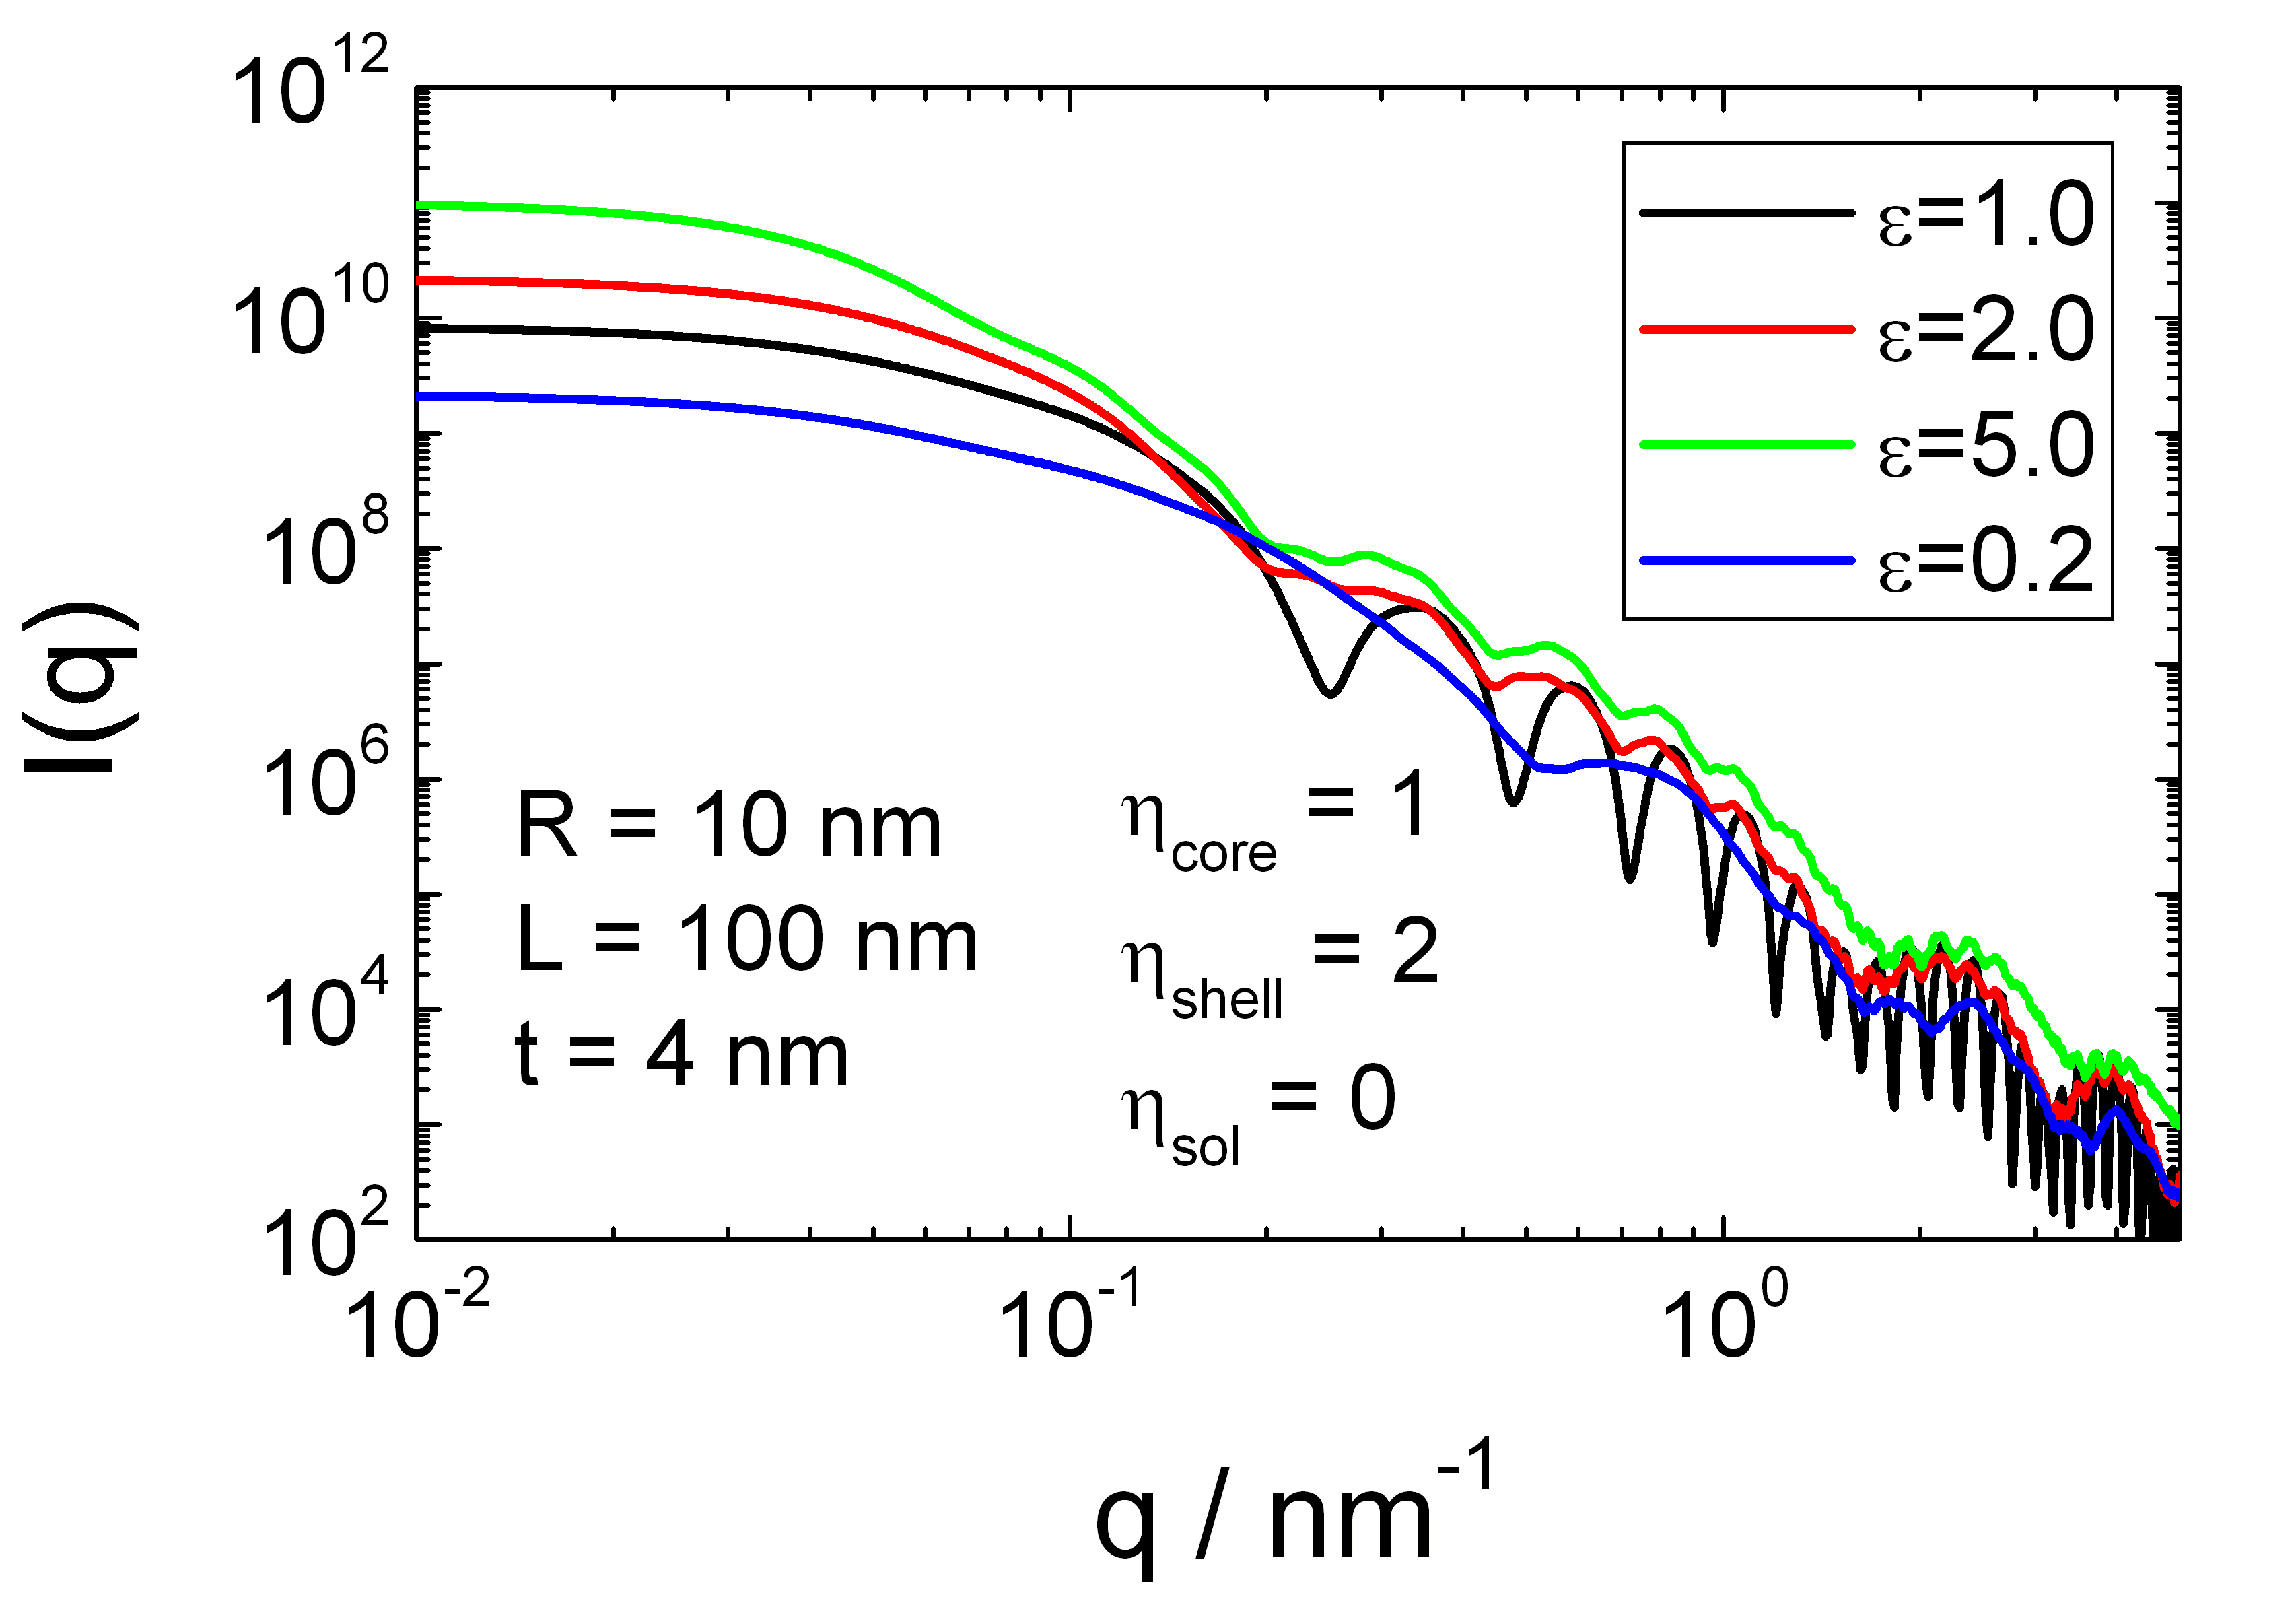
\includegraphics[width=0.65\textwidth,height=0.5\textwidth]{../images/form_factor/cylindrical_obj/ellCylShell1.png}
\end{center}
\caption{Scattering intensity of a cylinder with elliptical cross-section.}
\label{fig:ellCylShell1}
\end{figure}

\begin{figure}[htb]
\begin{center}
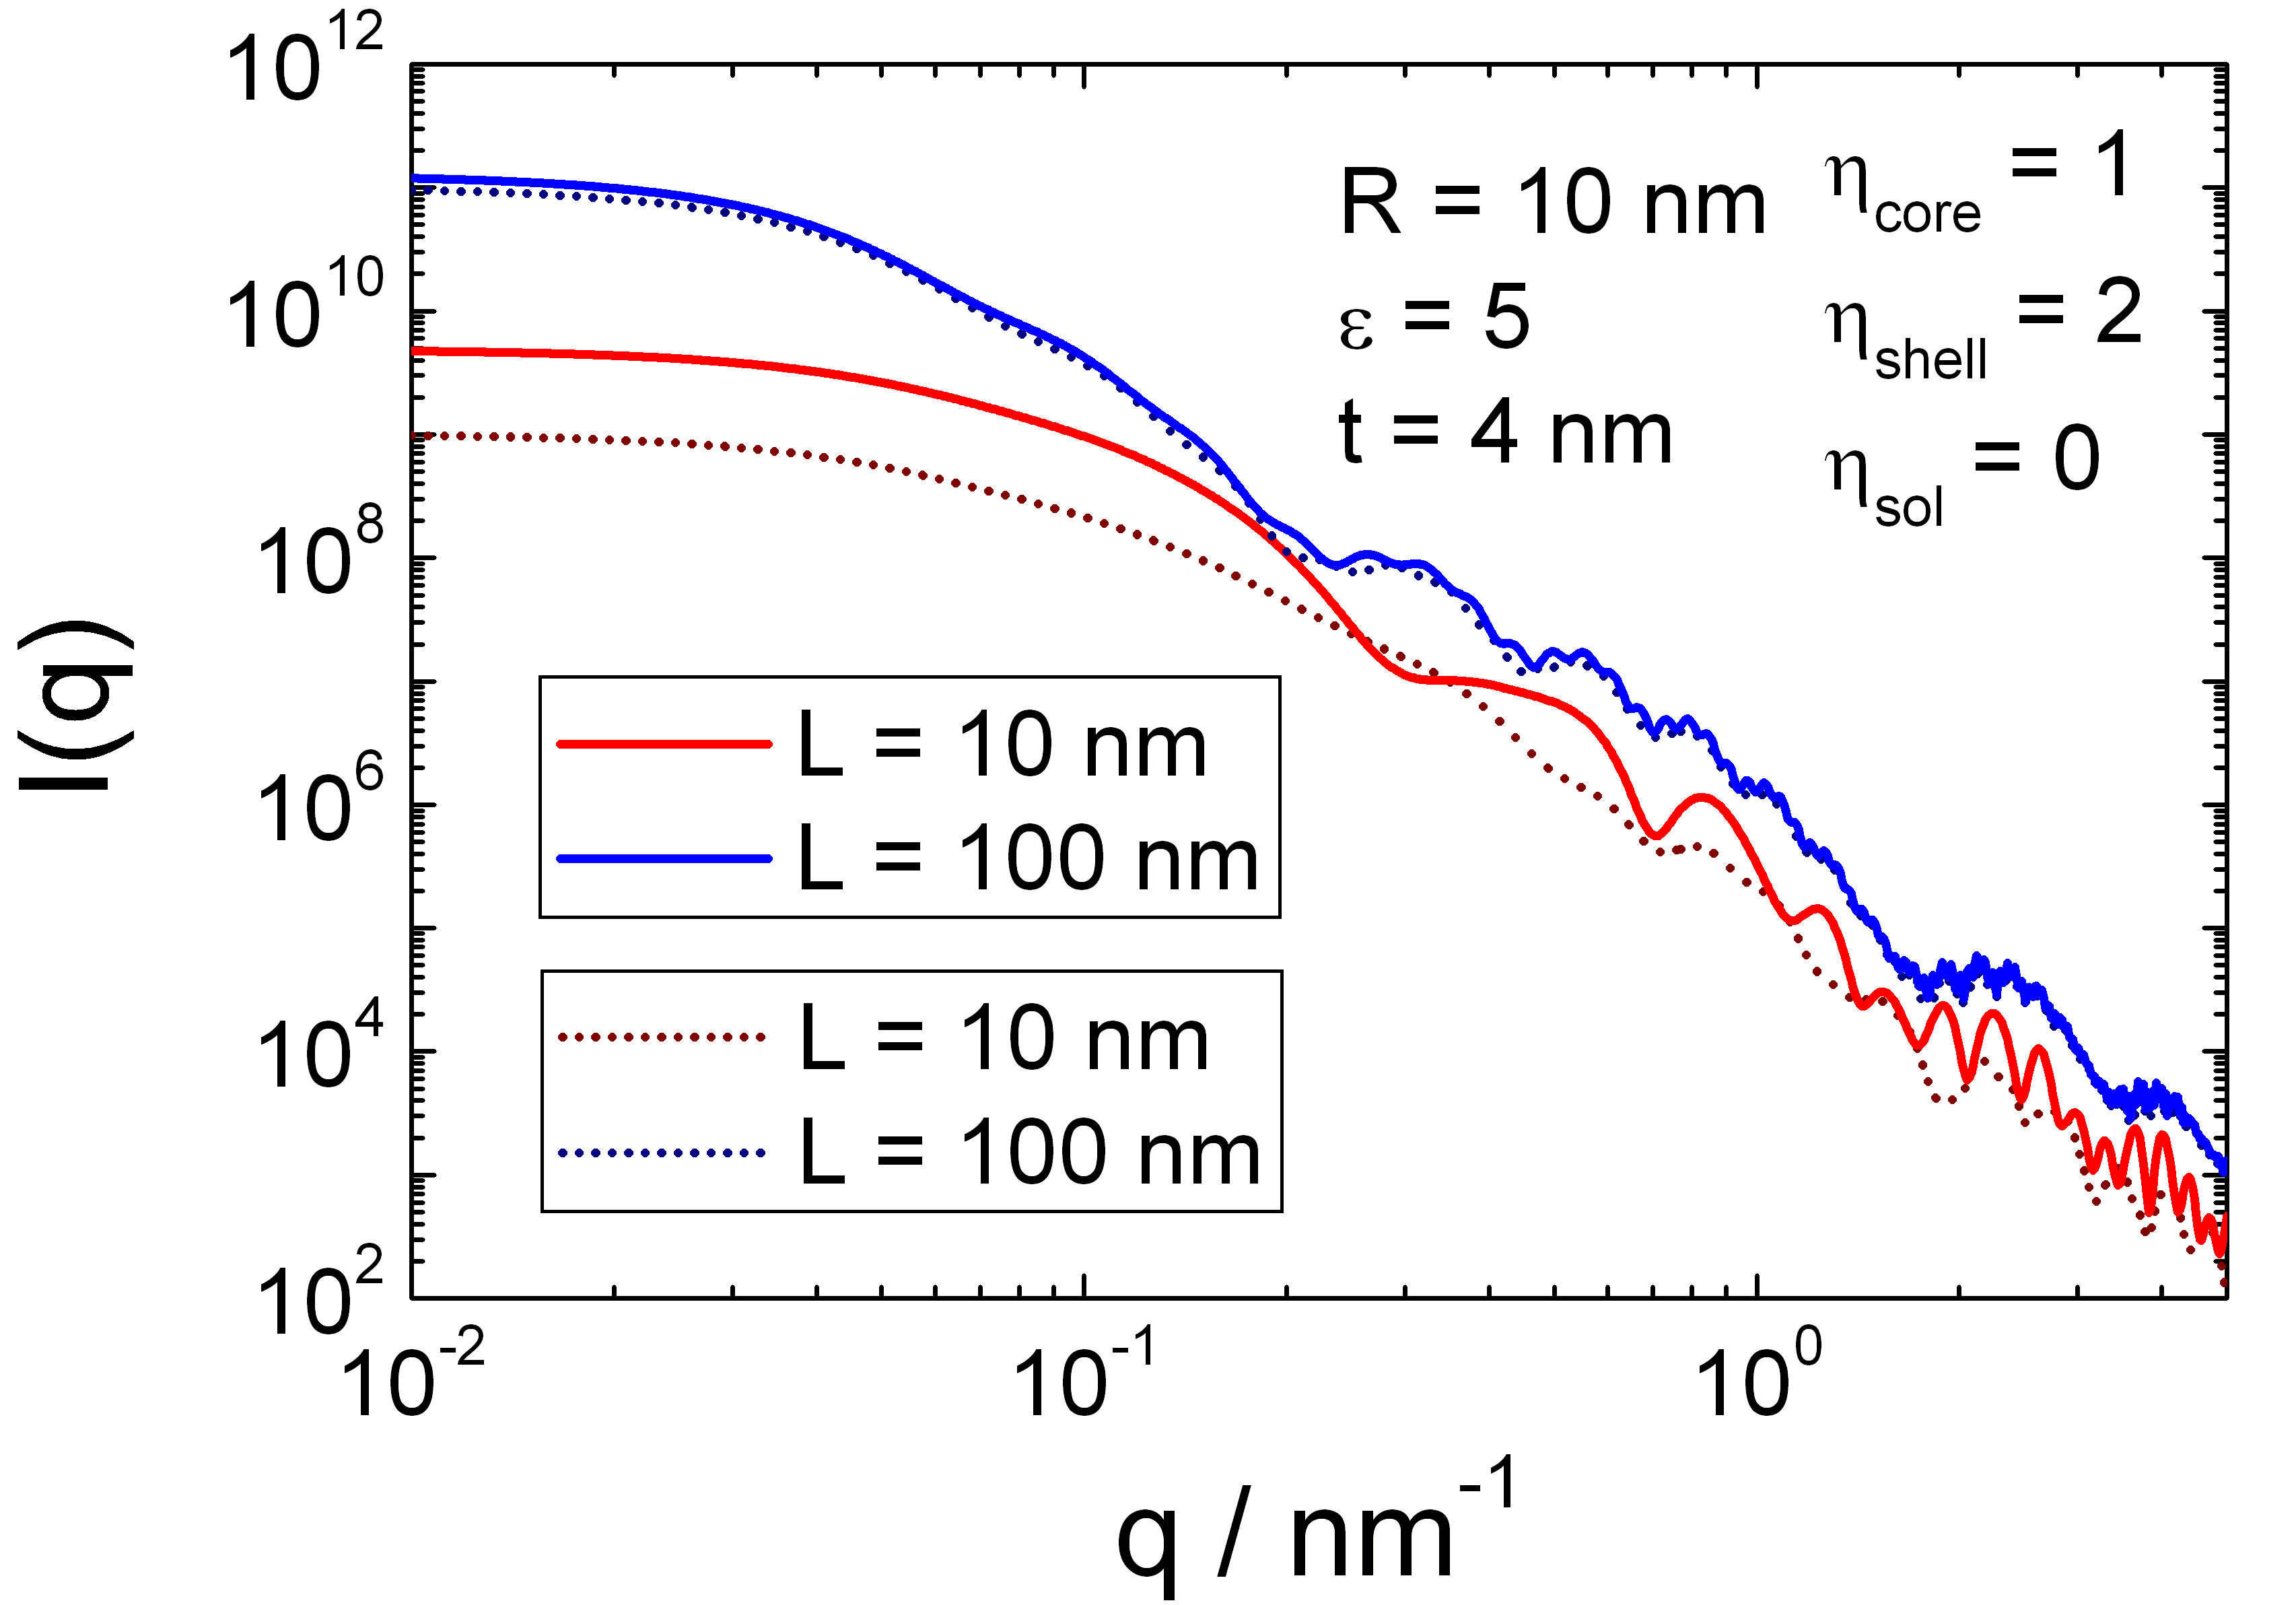
\includegraphics[width=0.65\textwidth,height=0.5\textwidth]{../images/form_factor/cylindrical_obj/ellCylShell1_2.png}
\end{center}
\caption{Scattering intensity of a cylinder with elliptical cross-section with and without capped ends.}
\label{fig:ellCylShell1_2}
\end{figure}

\vspace{5mm}

\noindent For very long cylinders a faster approximation for the
uncapped version can be used \texttt{Pcs:ellCylSh}
combined with the structure factor \texttt{P'(Q):Rod}.
The implemented approximation is the following
\begin{align}
  I_\text{Long\_ellCylShell}(q) = & P'(q) P_\text{cs}(q) \\
  P'(q)  = & 2 \frac{\text{Si}(q L)}{qL} - \left(\frac{\sin(qL/2)}{qL/2}\right) \\
  \text{Si}(x) & = \int_0^x\!\frac{\sin t}{t}\,\,dt \\
  r(R,\epsilon,\phi) &= \sqrt{R^2\sin^2(\phi)+(\epsilon R+t)^2\cos^2(\phi)}\\
  P_\text{cs}(q)  =  \frac{2}{\pi} \int_0^{\frac{\pi}{2}}& \biggl(
            \frac{2J_1(qr(R,\epsilon,\phi))}{qr(R,\epsilon,\phi)}
            \left(\eta_\text{core}-\eta_\text{shell}\right)\epsilon R^2L\pi + \\
         &
            \frac{2J_1(q(r(R,\epsilon,\phi)+t))}{Q(r(R,\epsilon,\phi)+t)}
            \left(\eta_\text{shell}-\eta_\text{sol}\right)(R+t)(\epsilon R+t)L\pi
      \biggr)^2  \, d\phi \nonumber
\end{align}

\hspace{1pt}\\
\underline{Input Parameters for model \texttt{Pcs:ellCylSh}:}\\
\begin{description}
\item[\texttt{R}] core radius $R$
\item[\texttt{epsilon}] eccentricity $\epsilon$ of cross-section
\item[\texttt{t}] shell thickness $t$
\item[\texttt{eta\_core}] scattering length density $\eta_\text{core}$ of cylinder core
\item[\texttt{eta\_shell}] scattering length density $\eta_\text{shell}$ of cylinder shell
\item[\texttt{eta\_sol}] scattering length density $\eta_\text{sol}$ of solvent
\end{description}

\begin{figure}[htb]
\begin{center}
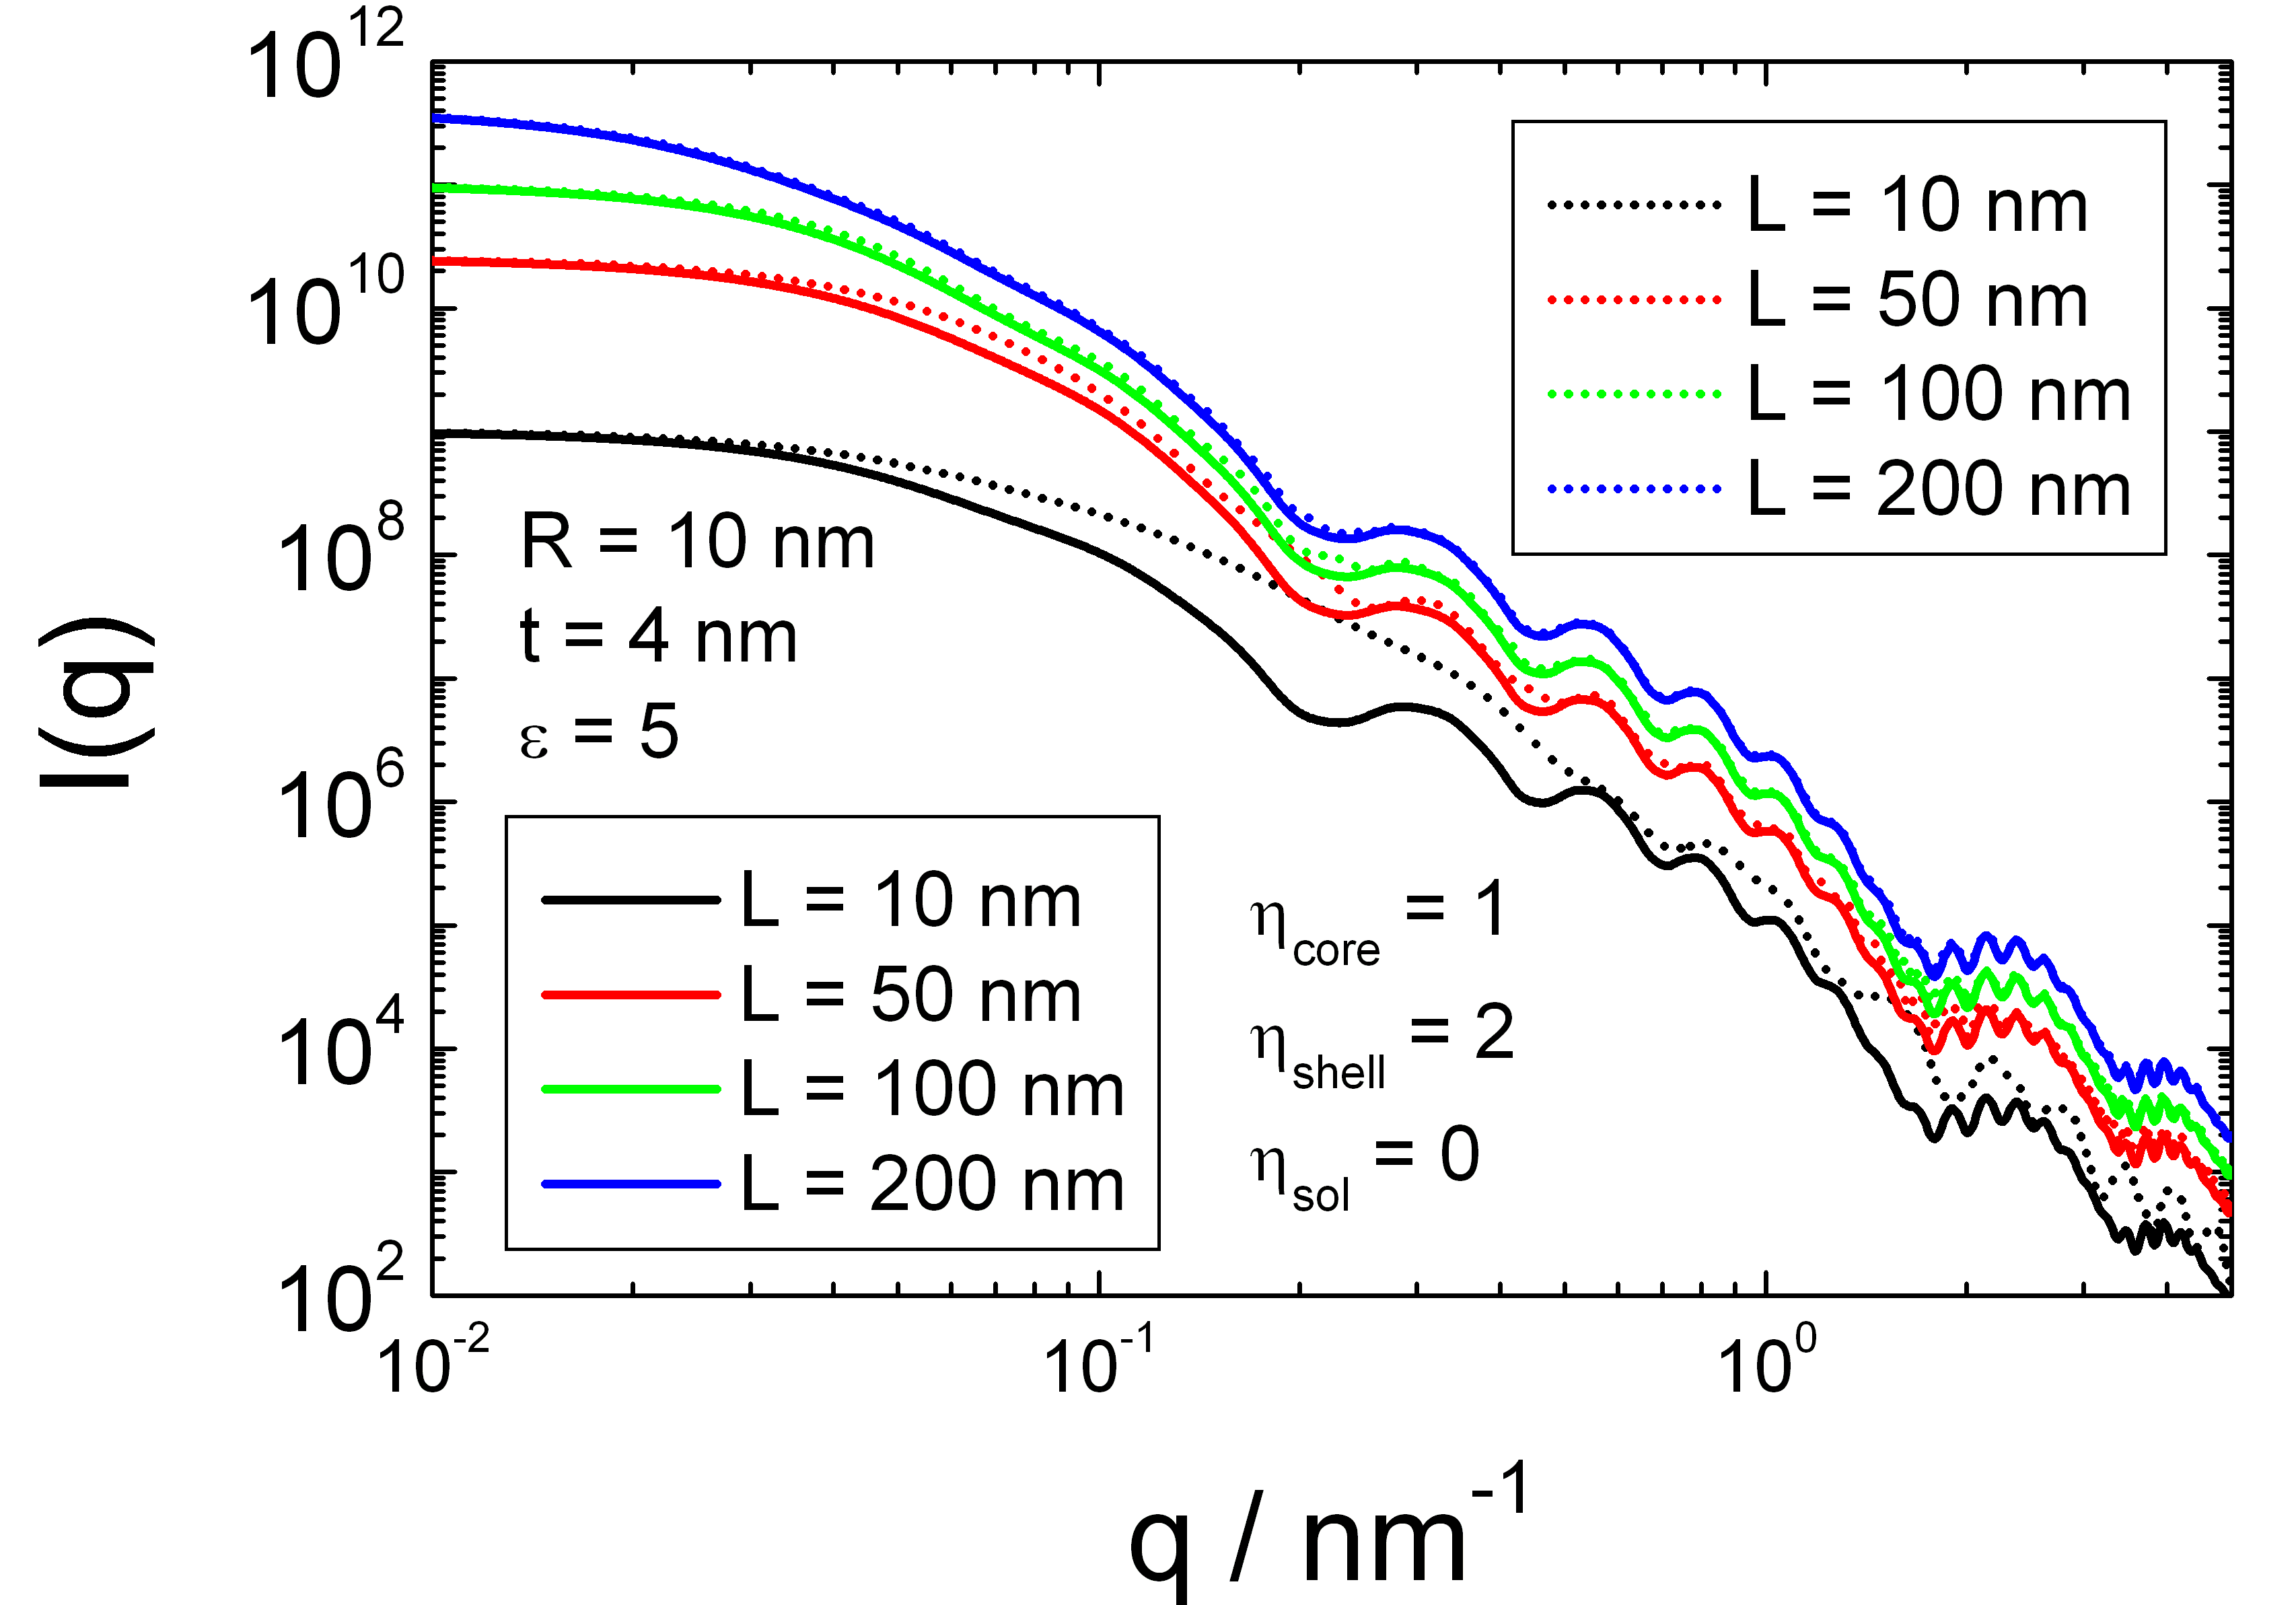
\includegraphics[width=0.65\textwidth,height=0.5\textwidth]{../images/form_factor/cylindrical_obj/Pcs_ellCylShell.png}
\end{center}
\caption{Scattering intensity of a cylinder with elliptical cross-section.
The exact solutions \texttt{ellCylShell1} (dotted lines) are compared
with \texttt{Pcs:ellCylSh} (solid lines), which is only valid for very long cylinders $L \gg 2R$. }
\label{fig:Pcs_ellCylShell}
\end{figure}


\clearpage

\subsection{partly aligned cylindrical shell \cite{Hayter1984}}
\label{sect:partlyalignedCylShell}
\hspace{1pt}\\
\begin{figure}[htb]
\begin{center}
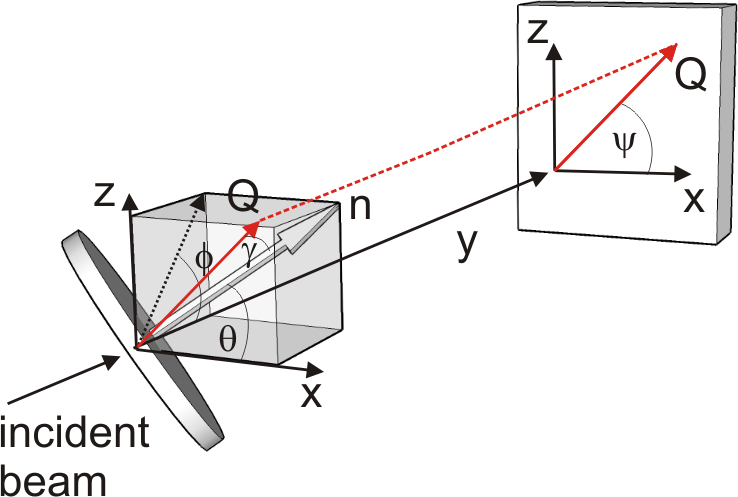
\includegraphics[width=0.786\textwidth,height=0.558\textwidth]{../images/form_factor/cylindrical_obj/partly_aligned_discs.png}
\end{center}
\caption{Sketch of relative orientation $\mathbf{n}$ of partly
aligned cylinders or discs to the scattering vector $\mathbf{Q}$.}
\label{fig:partly_aligned_discs}
\end{figure}

\noindent The scattering amplitude of a cylindrical shell is given by
\begin{align}
K_\text{CylShell}\left(Q,\dots,\gamma\right)  = &K_\text{Cyl}\left(Q,\eta_\text{core}-\eta_\text{shell},R,L,\gamma\right) \\
& +  K_\text{Cyl}\left(Q,\eta_\text{shell}-\eta_\text{solv},R+\Delta
R,L,\gamma\right)
\end{align}
with
\begin{align}
K_\text{Cyl}(Q,\Delta\eta,R,L,\gamma) & = 2 \pi R^2 L \Delta \eta
    \frac{J_1\left(Q R \sin\gamma\right)}{Q R \sin\gamma} \,
    \frac{\sin\left(\frac{QL}{2} \cos\gamma\right)}{\frac{QL}{2} \cos\gamma}
\end{align}
where $\gamma$ is the angle between $\mathbf{Q}$ and the cylinder
axis $\mathbf{n}$. $L$ is the length of the cylinder, $R$ its
radius, $\Delta\eta$ the scattering length density contrast relative
to the solvent and $J_1(x)$ is the first order Bessel function of
the first kind. $\gamma$ can be calculated from the orientation
($\theta$, $\phi$) of the cylinder and the direction of the
scattering vector $\psi$ in the plane of the detector by
\begin{align}
\frac{\mathbf{Q}}{\abs{\mathbf{Q}}} &=
\begin{pmatrix}
\cos \psi \\
0  \\
\sin \psi
\end{pmatrix} \qquad
\frac{\mathbf{n}}{\abs{\mathbf{n}}} =
\begin{pmatrix}
\cos \theta \\
\sin \theta \sin \phi  \\
\sin \theta \cos \phi
\end{pmatrix} \\
\cos \measuredangle(\mathbf{Q,n}) &= \cos \gamma = \frac{\mathbf{Q\cdot
n}}{\abs{\mathbf{Q}}\abs{\mathbf{n}}} = \cos\psi \cos\theta +
\sin\psi \sin\theta \cos\phi
\end{align}
If the orientation distribution of the orientation vector $\mathbf{n}$ is described by $p(\theta,\phi)$
so that the scattering intensity is given by
\begin{align}
I_\mathrm{p.a.CylShell}(Q) & =
            \int_0^\pi d\theta \int_0^{2\pi} d\phi \, \,
                K_\text{CylShell}\left(Q,\dots,\gamma\right)\,p(\theta,\phi)\,\sin(\theta)
\end{align}
For this form factor it is assumed that the orientation distribution is independent of $\phi$,
i.e. $p(\theta,\phi)=p(\theta)$ and that $p(\theta)=p(\pi-\theta)$, which means that turning
the cylinder by 180$^\circ$ results in the same scattering intensity. Instead of assuming a
special parametrization of $p(\theta)$ the orientation distribution was expanded in terms of
Legendre polynomials $P_l(\cos(\theta))$
\begin{align}
p(\theta) & = \sum_{l=0,even}^\infty \frac{2l+1}{2} \left\langle P_l\right\rangle\, P_l(\cos(\theta))
\end{align}
Due to the symmetrie $p(\theta)=p(\pi-\theta)$ all terms with odd values for $l$ are zero and only the
even terms needs to be considered. For this form factor the first three terms up to $l=6$ are implemented.
As $\int_0^\pi p(\theta) \sin\theta \, d\theta =1$ the zero order parameter is one $\left\langle P_0 \right\rangle=1$.


\vspace{5mm}

\hspace{1pt}\\
\underline{Input Parameters for model \texttt{partly aligned CylShell}:}\\
\begin{description}
\item[\texttt{R}] core radius $R$
\item[\texttt{DR}] shell thickness $\Delta R$
\item[\texttt{L}] cylinder length $L$
\item[\texttt{eta\_core}] scattering length density $\eta_\text{core}$ of cylinder core
\item[\texttt{eta\_shell}] scattering length density $\eta_\text{shell}$ of cylinder shell
\item[\texttt{eta\_solv}] scattering length density $\eta_\text{solv}$ of solvent
\item[\texttt{psi}] direction $\psi$ of the scattering vector in the plane of the detector
\item[\texttt{P2}] order parameter $\langle P_2\rangle$
\item[\texttt{P4}] order parameter $\langle P_4\rangle$
\item[\texttt{P6}] order parameter $\langle P_6\rangle$
\end{description}

\begin{figure}[htb]
\begin{center}
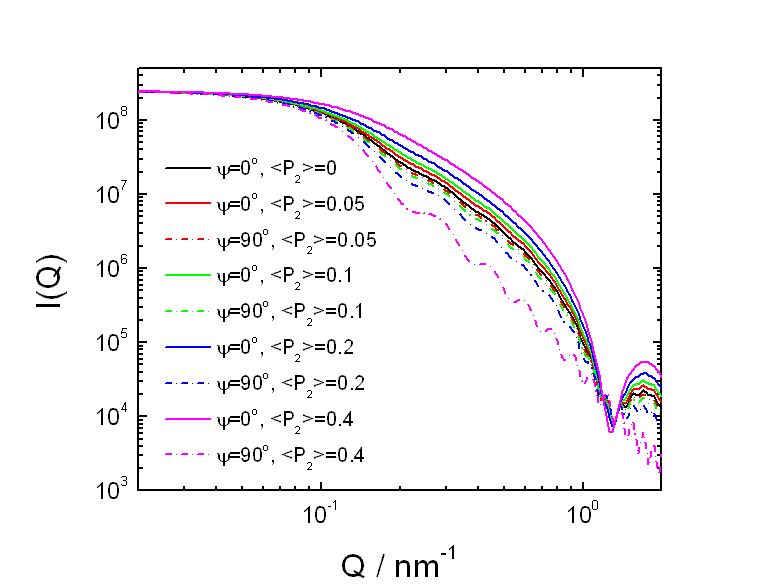
\includegraphics[width=0.786\textwidth,height=0.558\textwidth]{../images/form_factor/cylindrical_obj/partly_aligned_CylShell.png}
\end{center}
\caption{Scattering curve for partly aligned discs with radius $R=20$nm, $L=5$nm, $\Delta R=0$nm,
and $\left\langle P_2 \right\rangle=$0, 0.05, 0.1, 0.2, and 0.4. Higher order parameters are set
zero. $I(Q)$ is calculated for $\psi=0^\circ$ and $\psi=90^\circ$.}
\label{fig:partly_aligned_CylShell}
\end{figure}


%%%%%%%%%%%%%%%%%%%%%%%%%%%%%%%%%%%%%%%%%%%%%%%%%%%%%%%%%%%%%%%%%%%%%%%%%%%%%%%%%%%%%%%%%%%%
\newpage

\subsection{aligned cylindrical shell \cite{??}}
\label{sect:alignedCylShell}
\hspace{1pt}\\

%%%%%%%%%%%%%%%%%%%%%%%%%%%%%%%%%%%%%%%%%%%%%%%%%%%%%%%%%%%%%%%%%%%%%%%%%%%%%%%%%%%%%%%%%%%%
\newpage



\subsection{Torus with elliptical shell cross-section \cite{Kawaguchi2001,Forster1999}}
\label{sect:Torus}
\hspace{1pt}\\

\begin{figure}[htb]
\begin{center}
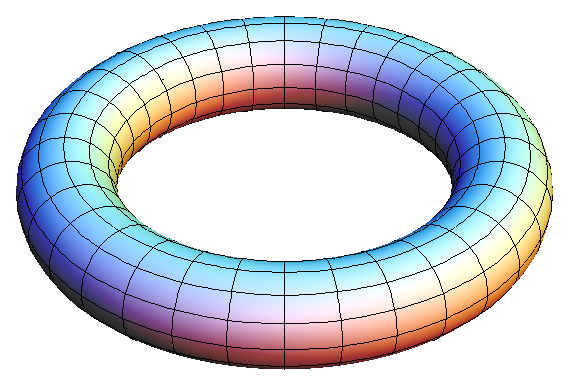
\includegraphics[width=0.575\textwidth,height=0.5\textwidth]{torus.png}
\end{center}
\begin{center}
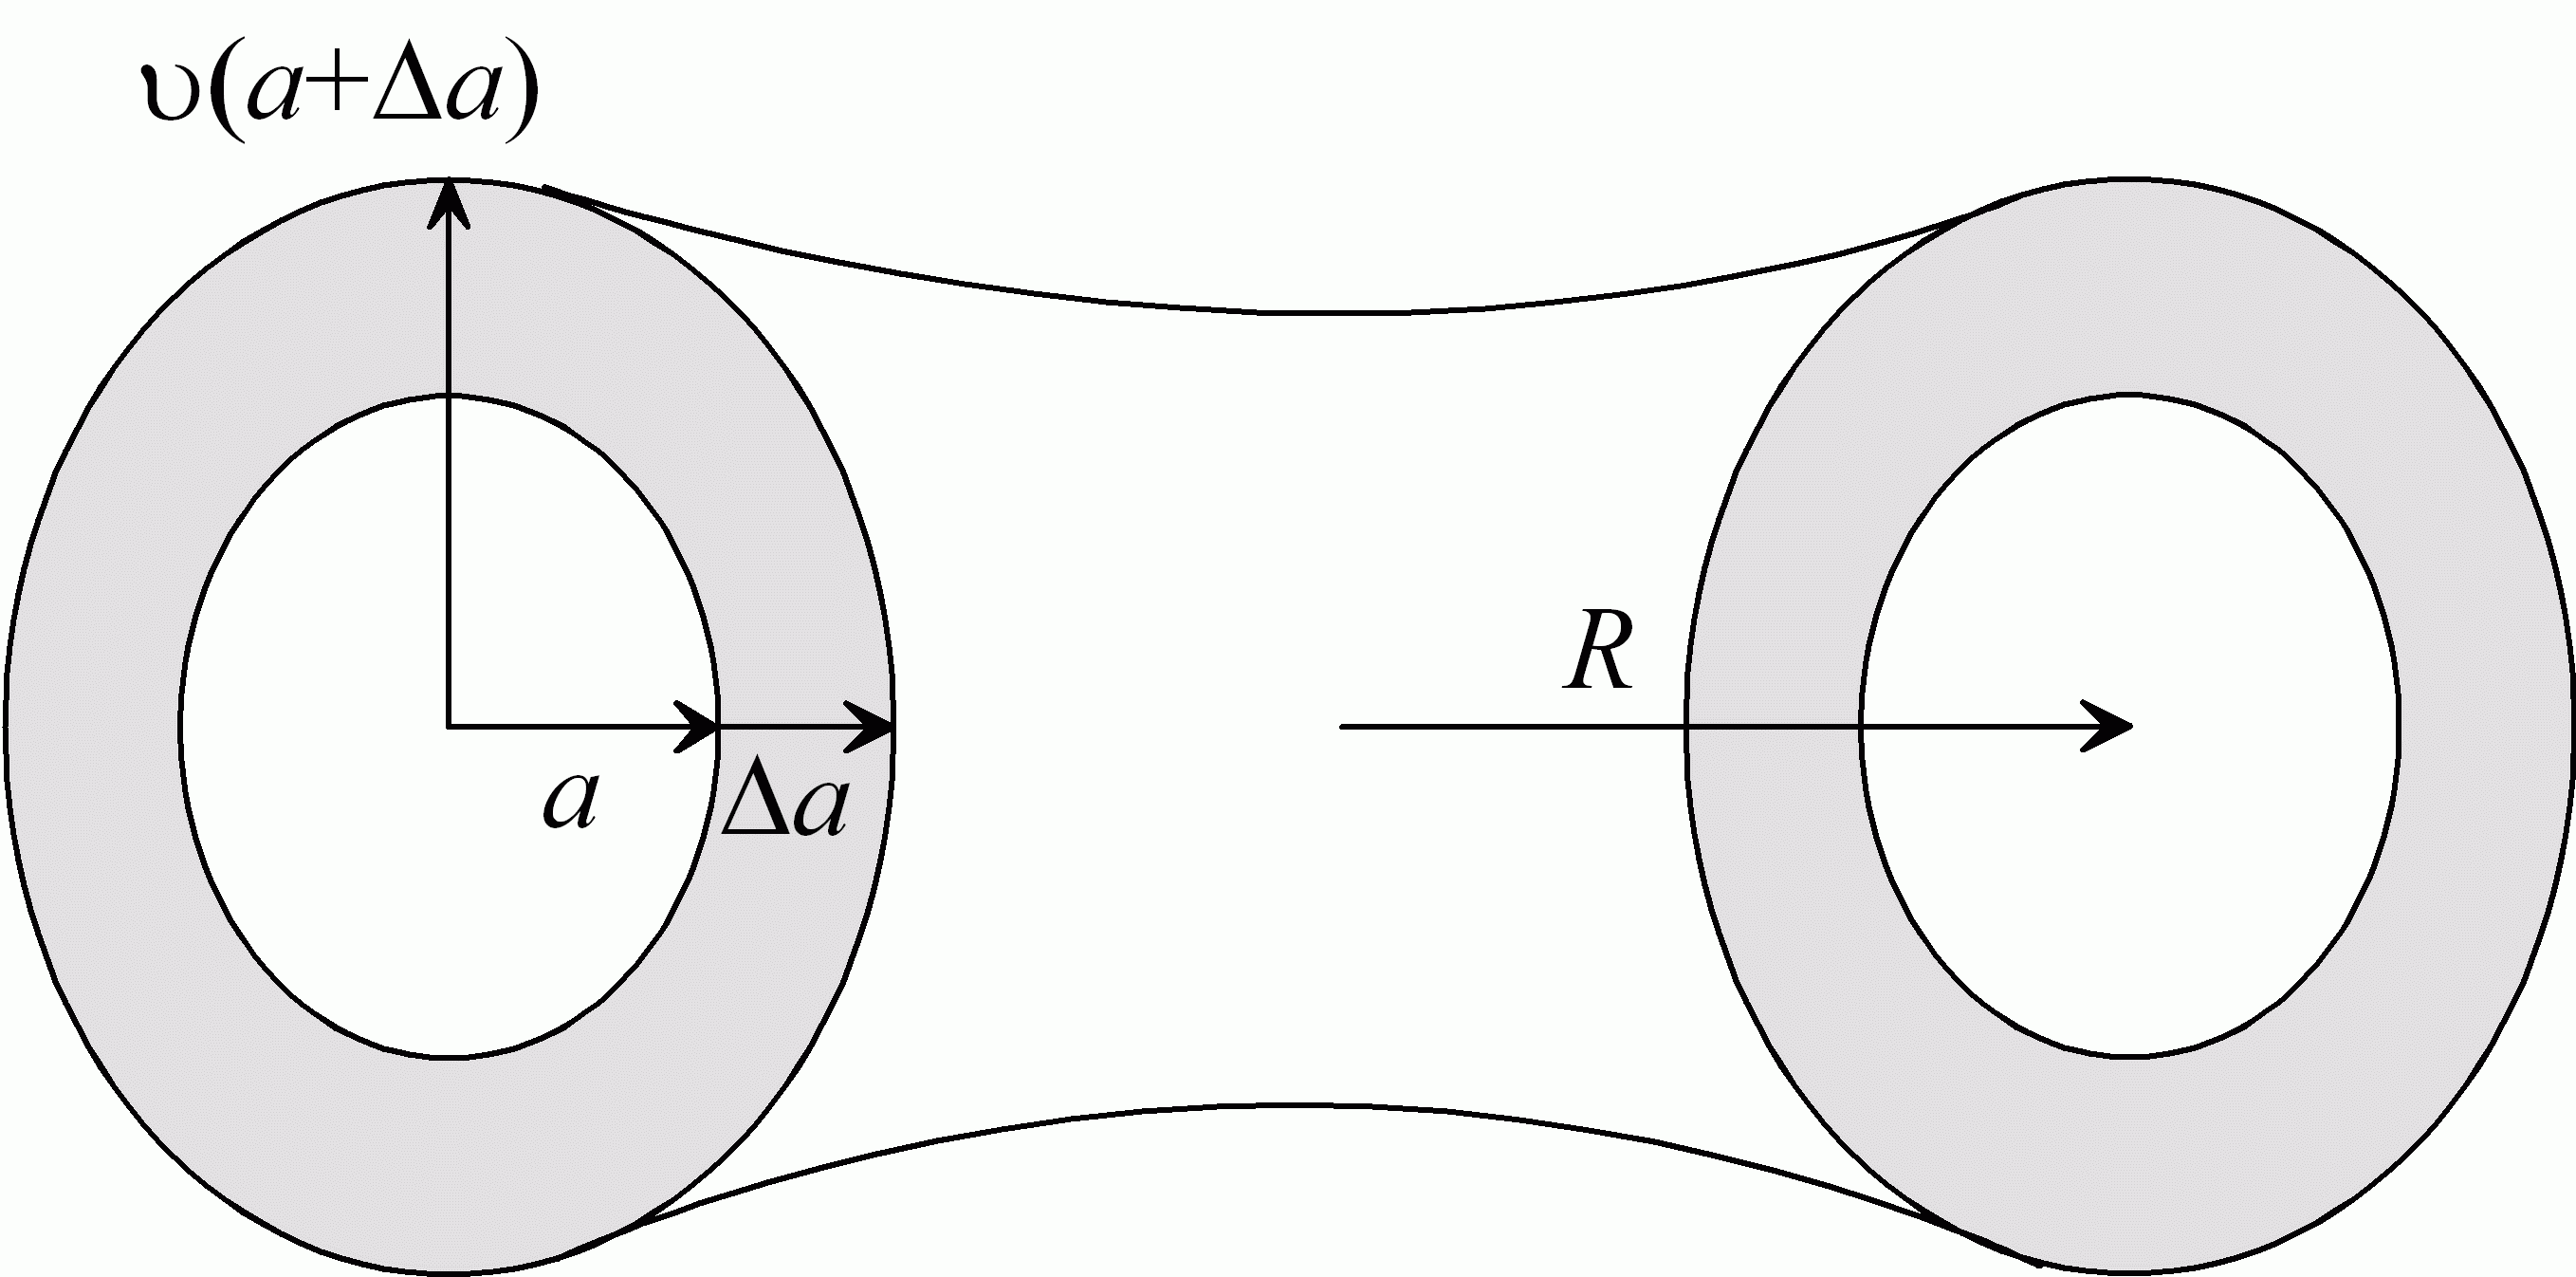
\includegraphics[width=0.6\textwidth,height=0.3\textwidth]{torus_sh_xsect.png}
\end{center}
\caption{} \label{torus}
\end{figure}
\begin{align}
F_\text{torus}(Q,\Theta,R,x,\nu,\Delta\eta) & = \int_{R-x}^{R+x}
4\pi r \Delta\eta \frac{J_0(Qr\sin\Theta) \sin(
Q\gamma(r)\cos\Theta)}{Q\cos(\Theta)} \; dr
\end{align}
\begin{align}
\text{with } \gamma(r) &= \nu \sqrt{x^2-(r-R)^2}
\end{align}
\begin{align}
I_\text{torus}(Q,R,a,\nu,\Delta\eta) &= \int_0^{\pi/2}
\abs{F_\text{torus}(Q,\Theta,R,a,\nu,\Delta\eta)}^2 \sin\Theta  \;
d\Theta
\end{align}
\begin{align}
I_\text{torus,sh}(Q,R,a,\Delta a,\nu,\Delta\eta_{sh},\Delta\eta_c)
= \int_0^{\pi/2} \Bigl\lvert & F_\text{torus}(Q,\Theta,R,a+\Delta
a,\nu,\Delta\eta_{sh}) \\
-&F_\text{torus}(Q,\Theta,R,a,\nu,\Delta\eta_c)\Bigr\rvert^2
\sin\Theta  \;  d\Theta \nonumber
\end{align}
An alternative form factor for $F_\text{torus}$ following \cite{Forster1999} is
\begin{align}
F_\text{torus}(Q,\Theta,R,x,\nu,\Delta\eta)  = 2\pi\int_{-x}^{x}
\bigg[
 & R_{(+)} J_1(QR_{(+)}\sin\theta) \\
-& R_{(-)} J_1(QR_{(-)}\sin\theta) \bigg]
\frac{\cos(Qz\cos\theta)}{Q\sin\theta} \; dz \nonumber
\end{align}
with $R_{(\pm)} = R\pm\nu\sqrt{x^2-z^2}$

\begin{figure}[htb]
\begin{center}
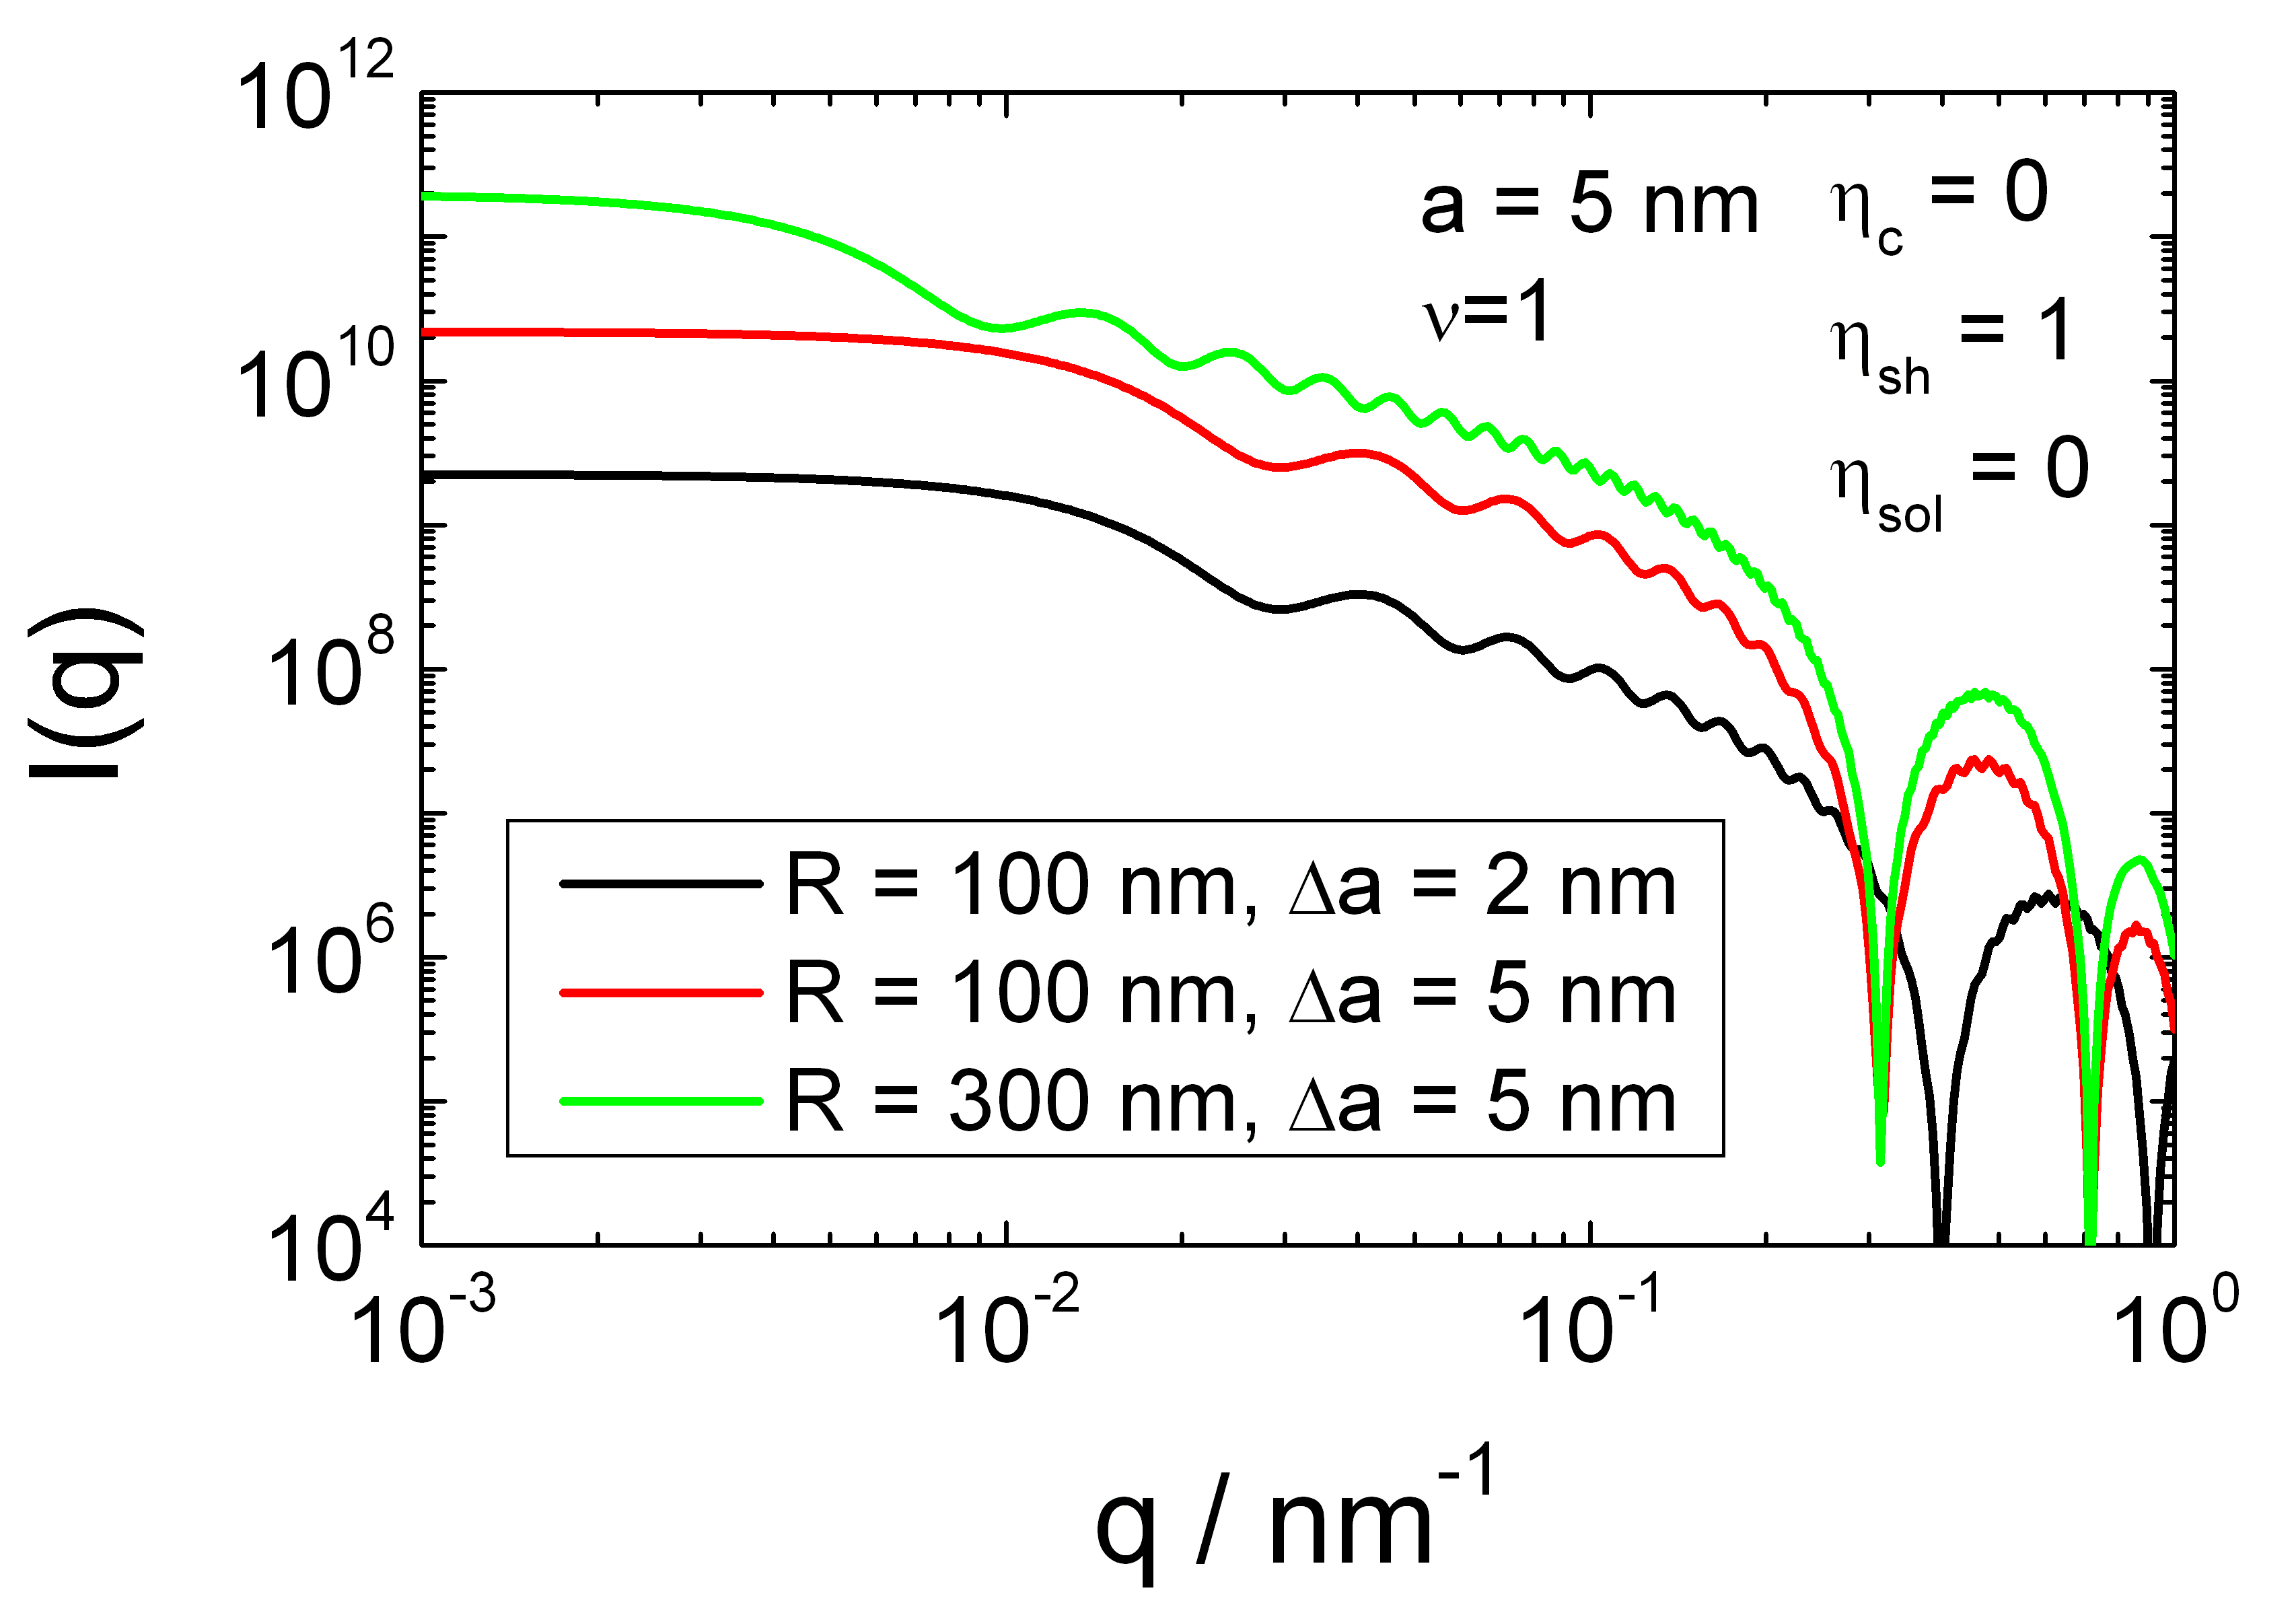
\includegraphics[width=0.65\textwidth,height=0.5\textwidth]{../images/form_factor/cylindrical_obj/Torus.png}
\end{center}
\caption{Scattering intensity of a torus. }
\label{fig:Torus}
\end{figure}


%%%%%%%%%%%%%%%%%%%%%%%%%%%%%%%%%%%%%%%%%%%%%%%%%%%%%%%%%%%%%%%%%%%%%%

\newpage
\subsection{stacked tori with elliptical shell cross-section} ~\\
\begin{figure}[htb]
\begin{center}
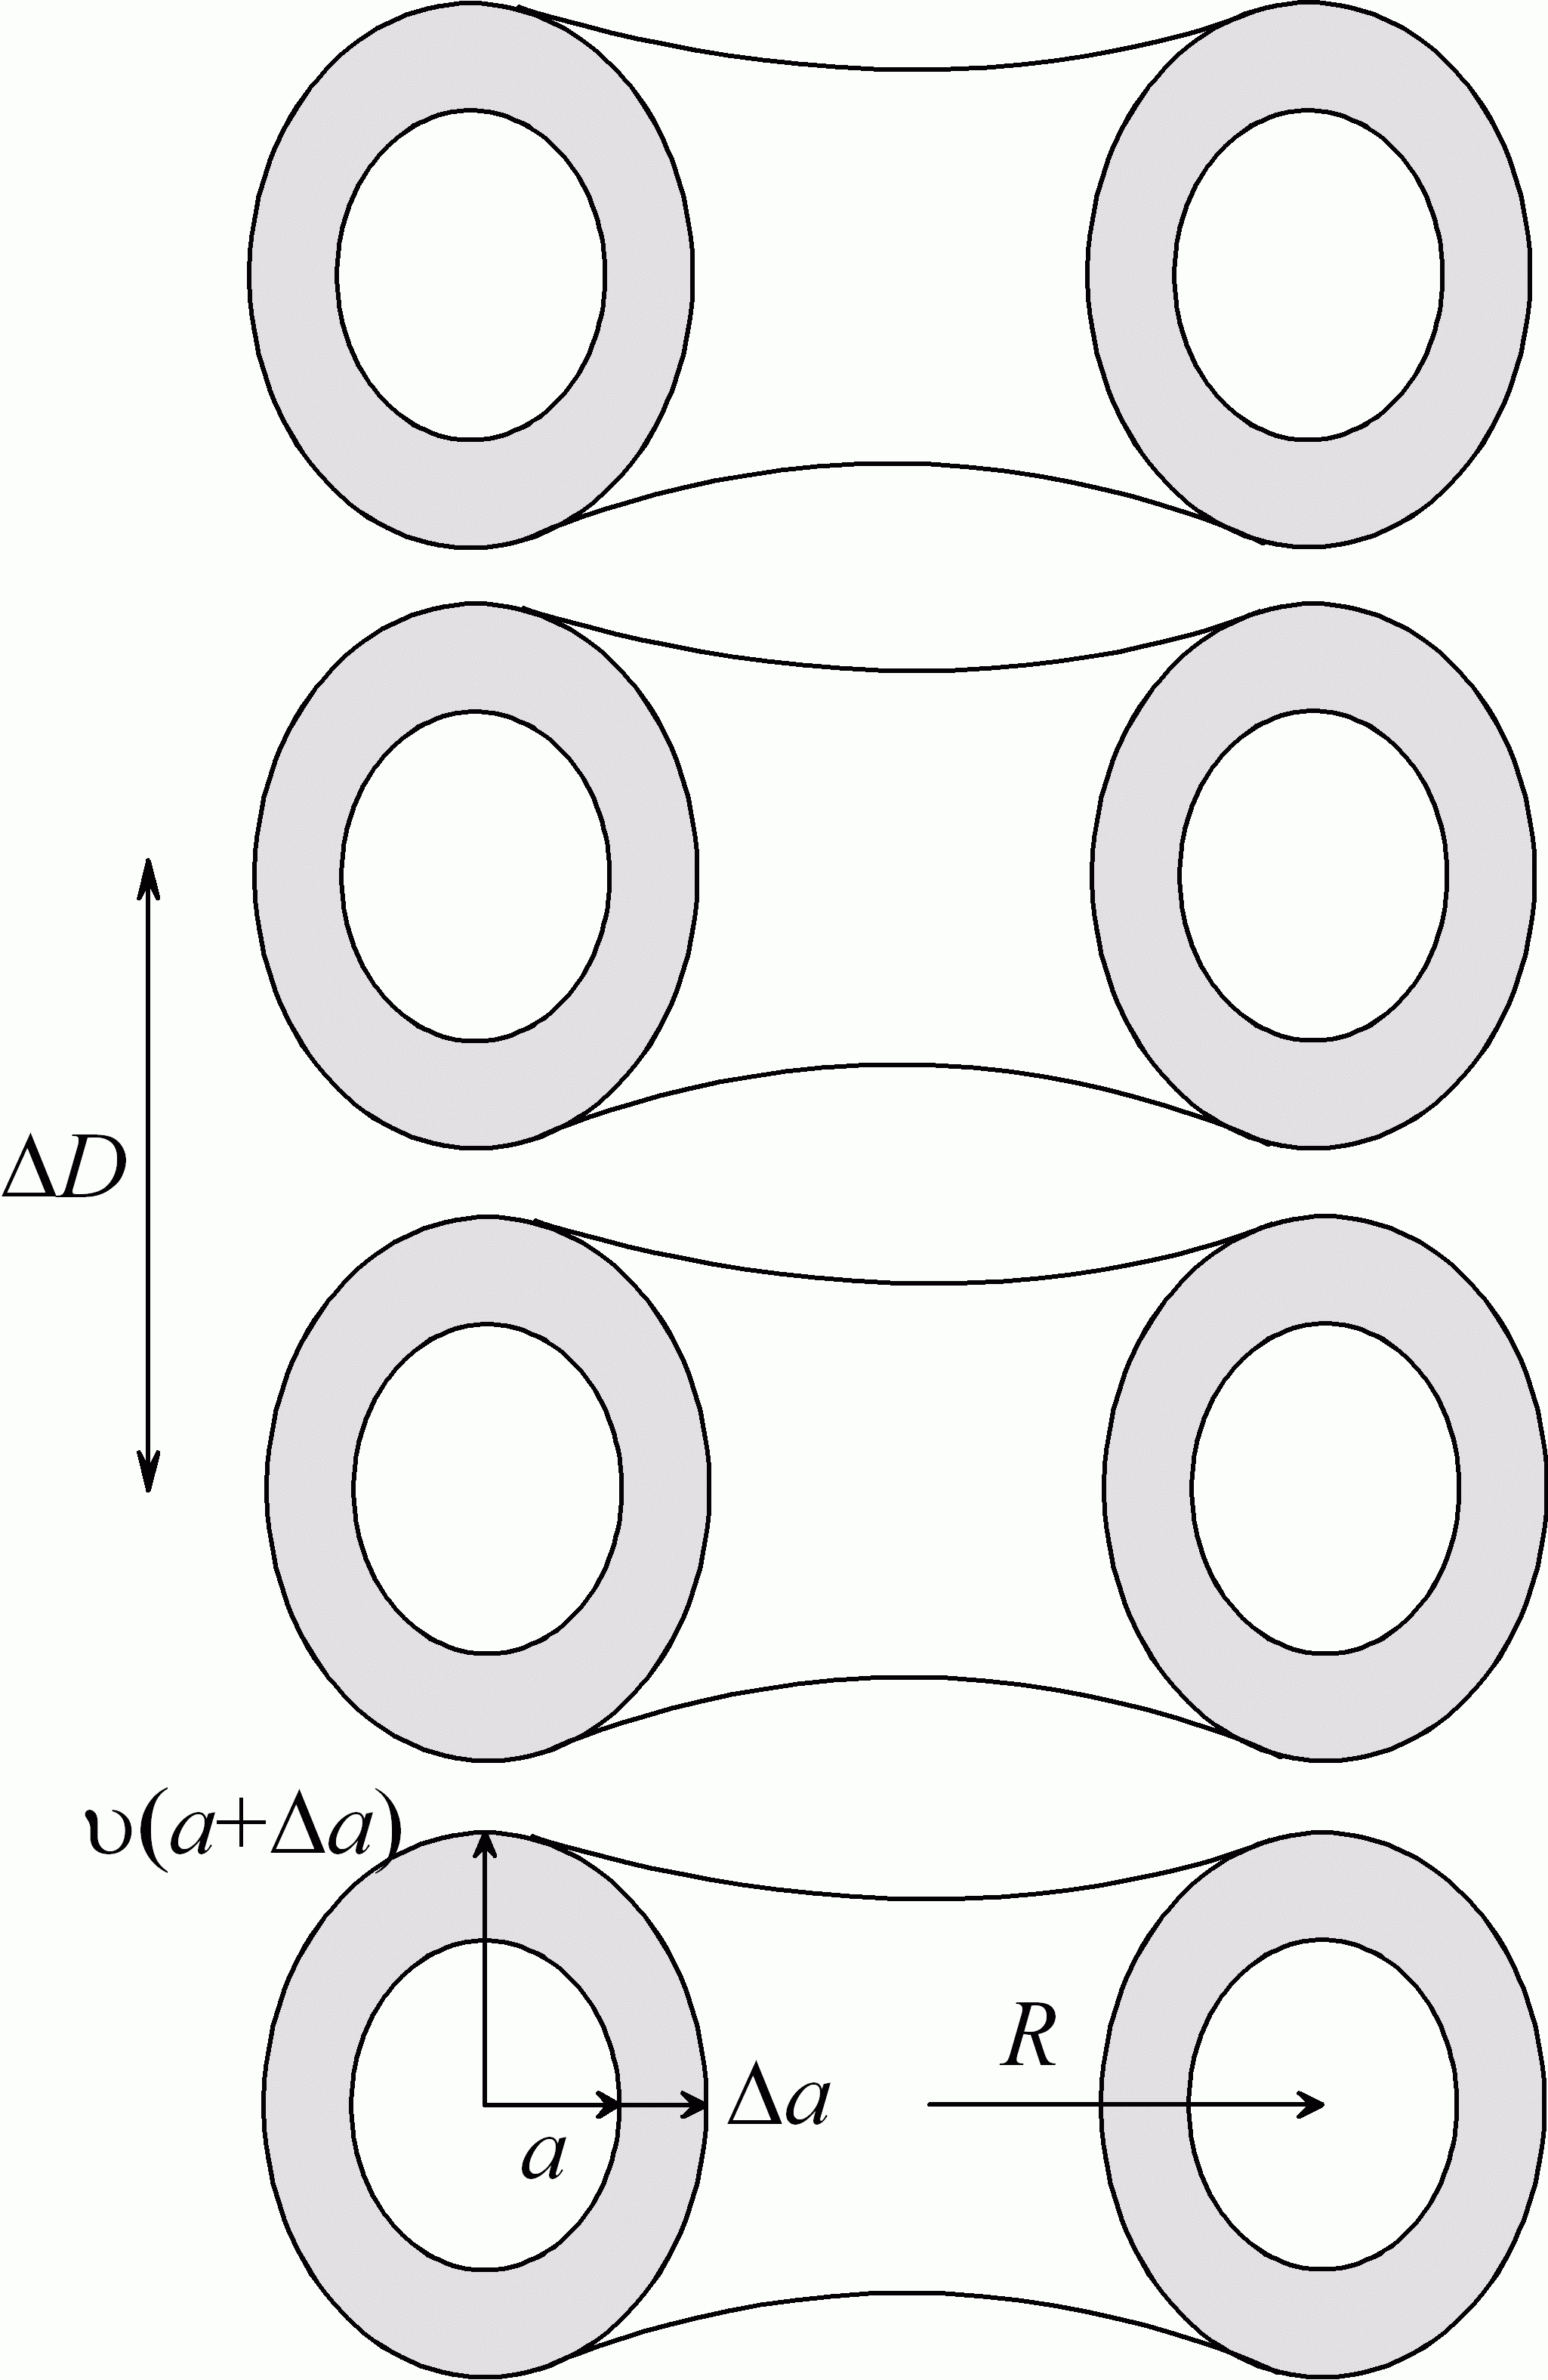
\includegraphics[width=0.55\textwidth,height=0.8\textwidth]{stacked_torus.png}
\end{center}
\caption{} \label{stackedTori}
\end{figure}
\begin{align}
F_\text{stacked} & _\text{tori}(Q,\Theta,R,x,\nu,\Delta\eta,\Delta D,N)  =  \\
& \sum_{n=1}^N \quad \int_{R-x}^{R+x} 4\pi r \Delta\eta
\frac{J_0(Qr\sin\Theta) \sin(
Q(\gamma(r)+\frac{2(n-1)-(N-1)}{4}\Delta
D)\cos\Theta)}{Q\cos(\Theta)} \; dr \nonumber
\end{align}
The scattering intensity is than calculated in the same way as for
a single torus with an elliptical shell cross-section.
